\documentclass[letterpaper, 11pt, oneside]{book}

\usepackage{graphicx} %Para imágenes
\usepackage[utf8]{inputenc} %Para configuración de caracteres
\usepackage[spanish]{babel} %Para configuración del idioma
\usepackage{anysize} %Para usar márgenes
\usepackage{tabularx} %Para que la tabla no se desborde
\usepackage{float} %Para que la tabla aparezca en otra hoja y en el lugar donde se quiere
\usepackage{multirow} %Para combinar filas
\usepackage{longtable} %Para que la tabla se divida en páginas
\usepackage{caption} %Espacio de la tabla y el titulo
\usepackage[table]{xcolor} %Colores tabla
\usepackage{csquotes}
\usepackage{hyperref}
\usepackage[backend=biber, style=ieee]{biblatex} %Bibliografía
\usepackage{array}
\addbibresource{Bibliografia.bib}

\marginsize{2cm}{2cm}{1cm}{2cm} %{izquierda}{derecha}{arriba}{abajo}
\newcolumntype{C}{>{\centering\arraybackslash}X} %Formato c y X de tabla
\definecolor{naranja}{HTML}{c1bebf}



\begin{document}
% Portada
\newcommand{\portada}{
    \begin{titlepage}
        \centering

        {\LARGE Desarrollo de módulos de mindset y fitness para el prototipo de plataforma enfocada en la enseñanza de habilidades blandas mediante gamificación. \par}

        \vfill
        {\large Juan Camilo Azcarate Cardenas}

        \vfill
        
\includegraphics[width=0.2\textwidth]{Imagenes/LogoUnivalle.png} % Ajusta el ancho de la imagen según tus necesidadesSF

        \vfill
        {\large Universidad del Valle \par
        Facultad de Ingeniería \par
        Escuela de Ingeniería de Sistemas y Computación \par
        Sede Tuluá \par
        2023 \par}
    \end{titlepage}
}
% Contraportada
\newcommand{\contraportada}{
    \begin{titlepage}
        \centering

        {\LARGE Desarrollo de módulos de mindset y fitness para el prototipo de plataforma enfocada en la enseñanza de habilidades blandas mediante gamificación. \par}

        \vfill
        {\large Juan Camilo Azcarate Cardenas \par
        Código 201958932 \par
        azcarate.juan@correounivalle.edu.co \par}



        \vfill
        {\large Director \par
        Msc Joshua David Triana Madrid\par
        joshua.triana@correounivalle.edu.co\par}

        \vfill
        
\includegraphics[width=0.2\textwidth]{Imagenes/LogoUnivalle.png}

        \vfill
        {\large Universidad del Valle, Sede Tuluá \par
        Facultad de Ingeniería \par
        Escuela de Ingeniería de Sistemas y Computación \par
        2023 \par}
    \end{titlepage}
}

\newcommand{\jurados}[3]{%
\thispagestyle{empty}
    \vspace*{4cm}
    \begin{center}
        Trabajo de grado presentado por \\[0.5cm]
        \textbf{#1} \\[0.5cm]
        Como requisito parcial para la obtención del título de \\[0.5cm]
        \textbf{Ingeniero de Sistemas}
    \end{center}
    \vfill
    \begin{center}
        \rule{70mm}{0.1mm} \\[0.2cm]
        \textbf{#2} \\[0.2cm]
        Director
    \end{center}
    \vfill
    \begin{center}
        \rule{70mm}{0.1mm} \\[0.2cm]
        \textbf{#3} \\[0.2cm]
        Jurado
    \end{center}
    \vfill
}

\newcommand{\agradecimientos}[1]{%
    \newpage
    \thispagestyle{empty}
    \begin{flushright}
        \textit{%
            Agradezco a mi familia por su apoyo durante todo el proceso y la confianza brindada.\\[0.5cm]
            A mis amigos por su constante ayuda y los buenos momentos durante la carrera.\\[0.5cm]
            Al profesor Joshua por su constante guía y consejos.\\[0.5cm]
            A los profesores por el conocimiento brindado a lo largo de la carrera.%
        }
    \end{flushright}
    \newpage
}


%Portada y contraportada
\portada
\contraportada
\jurados{Juan Camilo Azcarate Cardenas}{Msc Joshua David Triana Madrid}{}
\agradecimientos

%Tablas de contenido
\renewcommand{\contentsname}{Tabla de Contenido}
\tableofcontents
\thispagestyle{empty}

\renewcommand{\listfigurename}{Lista de Figuras}
\listoffigures 
\thispagestyle{empty}

\renewcommand{\listtablename}{Lista de tablas}
\listoftables
\thispagestyle{empty}

%Cuerpo del proyecto

%Resumen
\chapter*{Resumen}
Este proyecto tiene como meta ampliar un prototipo de plataforma existente que se enfoca en el desarrollo de habilidades blandas a través de la gamificación, específicamente para una plataforma gamificada para el aprendizaje de habilidades blandas en ingeniería de sistemas, la cual fue desarrollada simultáneamente con este proyecto por Daniel Felipe Cossio Marulanda. El objetivo de dicha plataforma es mejorar el desempeño académico y laboral de los estudiantes o profesionales de ingeniería de sistemas. La propuesta de este proyecto es integrar dos nuevos módulos específicos: 'Fitness', destinado al bienestar general, y 'Mindset', orientado a transformar las reacciones ante la vida de reactivas a proactivas. Estos módulos buscan complementar y enriquecer la experiencia de aprendizaje dentro del contexto de las habilidades blandas para estudiantes y profesionales de ingeniería de sistemas.
\\ \\
Las habilidades blandas, también llamadas habilidades interpersonales, son esenciales para el éxito en diversos ámbitos. Permiten una comunicación efectiva, la capacidad de resolver problemas, tomar decisiones, fomentar la innovación y liderar proyectos de manera eficaz al interactuar con otros individuos en cualquier entorno laboral o social.
\\ \\
Mientras tanto la gamificación es una táctica educativa que toma elementos característicos de los juegos y los implementa en entornos de aprendizaje y laborales con el propósito de mejorar los resultados. Busca facilitar la asimilación de conocimientos, fomentar el desarrollo de habilidades y premiar logros específicos, entre una variedad de objetivos adicionales. A través de este documento se evidenciará la gamificación para la enseñanza de habilidades blandas, específicamente para las habilidades blandas mindset y fitness, además contendrá los conocimientos necesarios para la comprensión de este proyecto.
\\ \\
\textbf{Palabras clave:} Soft Skills, habilidades blandas, gamificación, módulos.
\thispagestyle{empty}

%Abstract
\chapter*{Abstract}
This project aims to expand an existing platform prototype that focuses on the development of soft skills through gamification, more specifically for a gamified platform for learning soft skills for systems engineering, which was developed simultaneously with this project by Daniel Felipe Cossio Marulanda. The objective of this platform is to improve the academic and work performance of systems engineering students or professionals. The proposal for this project is to integrate two new specific modules: 'Fitness', aimed at general well-being, and 'Mindset', aimed at transforming reactions to life from reactive to proactive. These modules seek to complement and enrich the learning experience within the context of soft skills for systems engineering students and professionals.
\\ \\
Soft skills, also known as interpersonal skills, are essential for success in various fields. They enable effective communication, problem-solving abilities, decision-making, fostering innovation, and leading projects effectively by interacting with others in any work or social environment.
\\ \\
Meanwhile, gamification is an educational tactic that adopts characteristic elements of games and applies them in learning and work environments to enhance outcomes. It aims to facilitate knowledge assimilation, promote skill development, and reward specific achievements, among a variety of additional objectives. This document will showcase gamification for teaching soft skills, specifically for the mindset and fitness soft skills, and will also contain the necessary knowledge for understanding this project.
\\ \\
\textbf{Keywords:} Soft Skills, gamification, modules.


\thispagestyle{empty}

%Introducción
\setcounter{page}{1}
\chapter{Introducción}
Para desempeñarse de manera efectiva en la ingeniería de sistemas, se necesita mucho más que conocimientos técnicos o científicos. Las habilidades interpersonales, también conocidas como habilidades blandas, son fundamentales, ya que permiten una interacción fluida con otros individuos, la resolución de problemas, la toma de decisiones, la innovación y el liderazgo en proyectos. Entre las habilidades blandas esenciales para la ingeniería de sistemas se destacan la comunicación efectiva, el trabajo en equipo, la creatividad, el liderazgo y el pensamiento crítico.
\\ \\
En consecuencia es necesario encontrar nuevas estrategias didácticas que promuevan el desarrollo de habilidades blandas en los estudiantes o profesionales de ingeniería de sistemas. Una de ellas es la gamificación, la cual es una estrategia educativa que adopta elementos propios de los juegos en entornos de aprendizaje y trabajo para mejorar los resultados. Su objetivo es facilitar la absorción de conocimientos, el desarrollo de habilidades y la recompensa de logros específicos, entre otros muchos objetivos.\cite{b}
\\ \\
Ante ello, surge la necesidad de crear una plataforma de entrenamiento específica para el desarrollo de habilidades blandas, que brinde a los estudiantes universitarios la oportunidad de adquirir y perfeccionar estas destrezas esenciales para su futuro profesional.
Este proyecto tiene como propósito ampliar un prototipo de plataforma gamificada, diseñado por Daniel Felipe Cossio Marulanda, para el aprendizaje de habilidades blandas en ingeniería de sistemas, el cual fue desarrollado simultáneamente con este proyecto. La plataforma busca mejorar el desempeño académico y profesional de estudiantes y profesionales del área, promoviendo el desarrollo de estas habilidades mediante la gamificación. La ampliación incluye dos nuevos módulos centrados en las áreas de Fitness y Mindset.
\\ \\
El mindset, o mentalidad, refleja la perspectiva personal hacia la vida. Basado en el estoicismo, esta filosofía impulsa a tomar el control de tu existencia en lugar de depender de factores externos. Combinando influencias del estoicismo y el minimalismo, promueve una actitud proactiva en lugar de reactiva, alentando a asumir la responsabilidad y ser el protagonista de tu propia historia.
\\ \\
El fitness, o bienestar físico, es esencial para mantener nuestra salud en óptimas condiciones. En nuestro entorno laboral, pasamos largos periodos de tiempo en posiciones sedentarias, lo que puede acarrear importantes problemas de salud. Esta faceta del bienestar se concentra en aspectos vitales como la nutrición adecuada y la implementación de rutinas de ejercicio personalizadas.\cite{c}
\\ \\


%Formulación del problema
\chapter{Formulación del problema}



\section{Descripción del problema}
En la actualidad debido al crecimiento de personal calificado y graduado para tareas tecnológicas, las habilidades blandas o emocionales se han transformado en algo fundamental para el éxito profesional y personal, siendo estas las que permiten la interacción efectiva con los demás. Algunas de las habilidades blandas más demandadas por las empresas según los egresados universitarios son la proactividad, la capacidad de trabajo en equipo, la adaptabilidad, la inteligencia emocional y demás capacidades que ayudan a la toma de decisiones, solución de problemas e innovación de productos como se vio en el artículo de sobre Habilidades blandas y su importancia de aplicación en el entorno laboral.\cite{d}\\ \\

Estas habilidades consideradas fundamentales en la formación académica y laboral complementarias para el conocimiento técnico y científico son a menudo aquellas de las cuales no se recibe una adecuada educación durante los diferentes procesos de escolaridad. Los conocimientos más implementados durante la enseñanza en la universidad son de hecho los teóricos y prácticos, desestimando la importancia de competencias transversales que diversifiquen la aplicación del conocimiento en contextos reales. Esto a su vez genera una brecha entre los universitarios recién graduados y lo que en realidad se necesita en el mercado laboral.
\\ \\
En el caso específico de la ingeniería en sistemas, las habilidades blandas se vuelven aún más relevantes debido a la naturaleza colaborativa y multidisciplinaria del campo. Los ingenieros en sistemas no solo necesitan habilidades técnicas para diseñar, desarrollar e implementar soluciones tecnológicas, sino también competencias interpersonales que les permitan trabajar de manera eficiente en equipos y comunicarse con partes interesadas de diferentes niveles de experiencia técnica.
\\ \\
Estas habilidades son comúnmente solicitadas incluso de forma directa en diversos trabajos, un claro ejemplo ello se puede encontrar al usar aplicaciones enfocadas en la búsqueda de empleo como glassdoor el cual da decenas de miles de resultados para las soft skill o habilidades blandas en países como estados unidos o algunos cientos en países como el nuestro, como se demuestra a continuación:


\begin{figure}[ht]
  \centering
  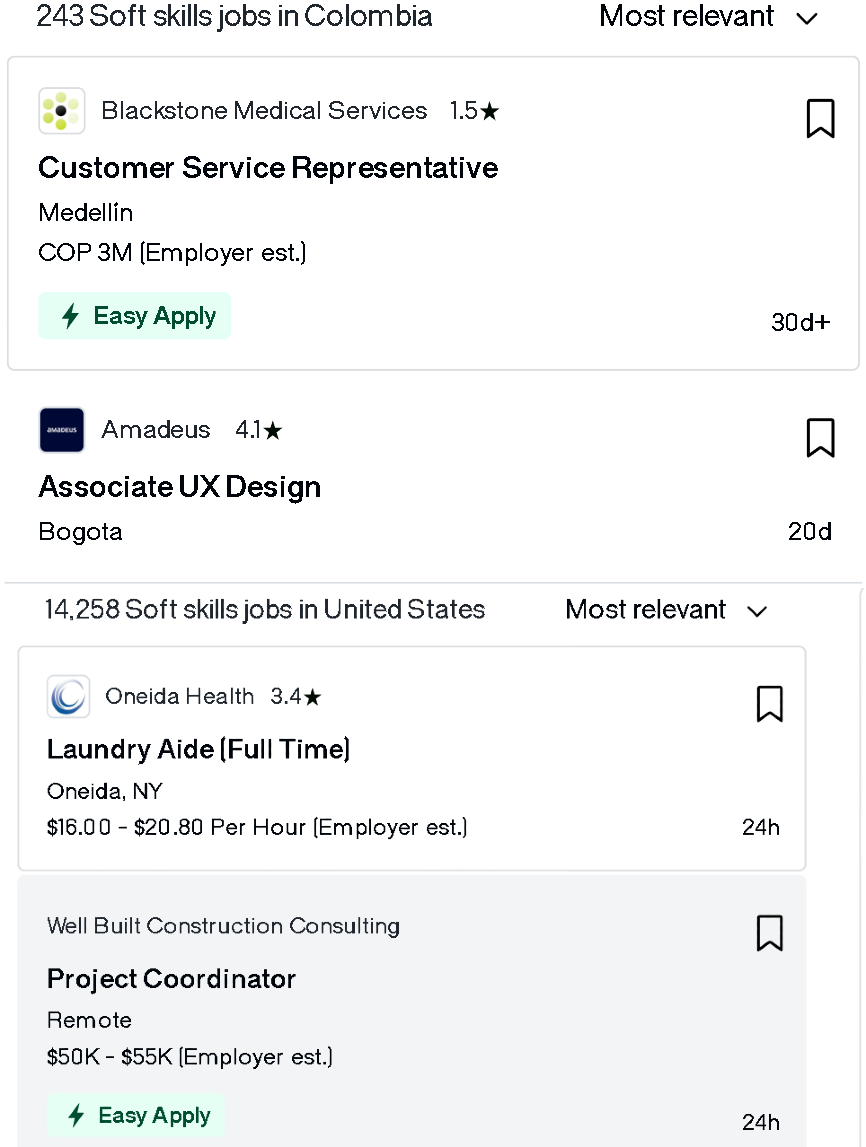
\includegraphics[width=0.5\linewidth]{Imagenes/glasdoor.png}
  \caption{Extraida de glasdoor\cite{q}}
  \label{fig:imagen}
\end{figure}
\newpage
Por consiguiente es necesario desarrollar las habilidades de los estudiantes de pregrado, para ello se puede optar por diferentes medios de educación como son el aprendizaje colaborativo que se basa formar un grupo con el objetivo aprender unos de otros, al discutir ideas y desarrollar habilidades sociales mientras resuelven problemas en conjunto o la gamificación la cual se refiere al uso y aplicación de mecánicas de juego en contextos no lúdicos la cual ha demostrado su eficacia en diferentes campos como la educación y la formación.
\\ \\
La gamificación en la educación tiene como objetivo principal transformar las experiencias de aprendizaje monótonas en actividades significativas y atractivas. Al integrar elementos de juegos en el proceso educativo, se busca motivar a los estudiantes a redescubrir la manera en que aprenden. Las clases que usan la gamificación están emergiendo como un método efectivo para comprometer a los estudiantes con un tema académico en particular. Este enfoque no solo reemplaza los métodos tradicionales, sino que también los mejora y revitaliza, ofreciendo una forma más dinámica de enseñanza.
\\ \\
La gamificación va más allá de simplemente otorgar puntos o premios en clase. Su verdadero potencial radica en convertir el entorno educativo en una experiencia divertida y enriquecedora, donde se exploran las pasiones y motivaciones de los estudiantes. Esta metodología permite comprender mejor a los alumnos, ya que un enfoque educativo desprovisto de elementos gamificados limita su participación activa. Integrar estrategias gamificadas no solo impulsa la participación estudiantil, sino que también crea un ambiente didáctico motivador, enriquecido con la emoción de la sorpresa y la gratificación.\cite{e}
\\ \\
Es verdad que, a pesar de la eficacia demostrada de estos métodos de enseñanza, a menudo enfrentan desafíos en términos de su disponibilidad y desarrollo centralizado en plataformas accesibles para su uso generalizado.
\section{Formulación del problema}
En consecuencia en búsqueda de describir el problema  y hallar una idea más clara se llega al siguiente interrogante.
\\ \\
¿Cuál sería la metodología para el diseño y la gamificación de dos módulos centrados en las habilidades 'fitness' y 'mindset' destinados a ser integrados en un prototipo de plataforma web?

%Marco de referencia
\chapter{Marco de referencia}
%Marco teórico
\section{Marco Teórico}
\begin{itemize}
    \item \textbf{Aprendizaje basado en juegos:} Se analiza teoría de aprendizaje basado en juegos, La cual se refiere a la utilización de juegos como parte integral del procesos educativo, apoyando un entorno más interactivo y significativo en la adquisición del conocimiento. Investigando sus diferentes componentes como son la progresión lineal, la fomentación del aprendizaje, participación activa y la retroalimentación instantánea.
    \\ \\
Esta metodología tiene como finalidad última utilizar juegos con el fin de aprender a través de ellos. El juego se convierte en el vehículo para realizar un aprendizaje o para trabajar un concepto determinado. Mientras dura el juego, o al final de la partida, el docente puede reflexionar en torno a lo que está sucediendo en el juego y los contenidos que se quieren trabajar.\cite{f}

\end{itemize}

\begin{itemize}
    \item \textbf{Gamificación:} En primer lugar conviene expresar que en este proyecto  se utiliza el término gamificación en lugar de ludificación, además se analiza la definición y los principios fundamentales de la gamificación.
    \\ \\
La gamificación es el intento estratégico de mejorar sistemas, servicios, organizaciones y actividades al crear experiencias similares a las experimentadas al jugar juegos, con el fin de motivar e involucrar a los usuarios. Generalmente, esto se logra aplicando elementos de diseño de juegos y principios de juegos (dinámicas y mecánicas) en contextos no relacionados con juegos.\cite{g}
\\ \\
La gamificación forma parte del diseño de sistemas persuasivos y comúnmente utiliza elementos de diseño de juegos para mejorar la participación de los usuarios, la productividad organizacional, el flujo de trabajo, el aprendizaje, la colaboración colectiva, la retención de conocimientos, la contratación y evaluación de empleados, la facilidad de uso, la utilidad de los sistemas, el ejercicio físico, las infracciones de tráfico, la apatía electoral, las actitudes públicas hacia la energía alternativa, entre otros aspectos. Una recopilación de investigaciones sobre gamificación muestra que la mayoría de los estudios encuentran efectos positivos en las personas. Sin embargo, existen diferencias individuales y contextuales.
\\ \\
Uno de los principios básicos para la gamificación es el del MDA, uno de los marcos de referencia más prevalentes y empleados en la actualidad para el diseño y evaluación de juegos, se centra en los tres pilares fundamentales de cualquier juego: las mecánicas, las dinámicas y las estéticas.
\\ \\
Las mecánicas de juego se refieren a las reglas que transforman una actividad en una experiencia lúdica o de juego. Estas reglas fomentan la participación y el compromiso de los usuarios al plantear una serie de desafíos y obstáculos que deben superar.
\\ \\
Las dinámicas de juego abarcan los aspectos y valores que moldean la percepción de una actividad. Estos elementos se seleccionan en función del objetivo que se busca alcanzar, como la progresión, la narrativa, la colaboración, entre otros.
\\ \\
La estética del juego se relaciona con el entorno, plataforma o interfaz que permite la experiencia de juego. Se centra en el diseño de la experiencia del usuario, lo cual determina el nivel de atracción que generará en el usuario. Esto abarca tanto los aspectos visuales como táctiles y auditivos de la experiencia de juego.


\end{itemize}
\begin{itemize}
    \item \textbf{Habilidades blandas:}
 Se descomponen e investigan las habilidades blandas también llamadas habilidades sociales o habilidades interpersonales, las cuales afectan la manera como realizamos tareas o interactuamos con los demás, como son la resolución de conflicto, el liderazgo, el trabajo en equipo. 
 \\ \\
Estas capacidades específicas se refieren a habilidades que pueden mejorar el rendimiento laboral, promover la progresión profesional y prever el éxito en el trabajo. También se conocen con diversos nombres como competencias para el siglo XXI, habilidades genéricas, habilidades socioemocionales, entre otros. Estas capacidades abarcan habilidades sociales, interpersonales y metacompetencias que permiten trabajar en entornos diversos y transferir conocimientos de un área a otra.\cite{h} Se examinan estas habilidades, su importancia en el entorno laboral y la vida cotidiana.

\end{itemize}

\begin{itemize}
    \item \textbf{Diseño de experiencia de usuario:}
Se emplea el análisis teórico y práctico del diseño de la experiencia del usuario en relación con la gamificación para desarrollar y aplicar este concepto. Se explorarán aspectos como accesibilidad, usabilidad y diseño de interfaz con el objetivo de ofrecer una experiencia más atractiva y motivadora. 
\end{itemize}

\begin{itemize}
    \item \textbf{Evaluación del aprendizaje:}  Se exploran tácticas y enfoques destinados a medir el progreso de los usuarios en entornos de aprendizaje gamificados. Esto incluye el diseño de métodos que permitan evaluar de manera efectiva tanto el desempeño como el avance en el desarrollo de habilidades. Se enfatiza la importancia de implementar evaluaciones continuas para identificar áreas de mejora, así como la recopilación y análisis de datos relevantes. Estos datos no solo proporcionan una visión integral del progreso, sino que también sirven para personalizar la experiencia de aprendizaje, ajustar las estrategias utilizadas y garantizar que la plataforma cumpla con sus objetivos educativos.

\end{itemize}

\begin{itemize}
    \item \textbf{Teoría de sistemas:} “La Teoría General de Sistemas se concibe como una serie de definiciones, de suposiciones y de proposiciones relacionadas entre sí por medio de las cuales se aprecian todos los fenómenos y los objetos reales como una jerarquía integral de grupos formados por materia y energía;estos grupos son los sistemas.
     \\ \\
Un sistema es un conjunto de fenómenos de objetos con relaciones estrechas entre los unos y los otros y entre los atributos de los mismos. Los sistemas pueden ser de diversidad enorme. La molécula, la célula, el individuo, los grupos sociales, la sociedad y las naciones son todos ejemplos de sistemas vivientes y podrían citarse ejemplos de sistemas no vivientes y muchos también de sistemas combinados que son, por lo demás, los más importantes (sistemas hombre-máquina, por ejemplo).”\cite{i}


\end{itemize}

%Marco conceptual
\section{Marco conceptual}
\begin{itemize}
    
    \item \textbf{Gamificación en la educación:}
    La gamificación ha demostrado su efectividad en la educación, y se han realizado investigaciones que demuestran resultados positivos en el desarrollo de habilidades blandas a través del uso de un enfoque gamificado, como bien lo ha demostrado la revista Ra Ximhai\cite{j} en el caso de la motivación en un aula presencial, sin embargo su uso en  plataformas específicas para el entrenamiento de habilidades blandas es un campo actualmente en crecimiento y que requiere de más investigaciones.
    \item \textbf{Plataformas de e-learning:} Existen un gran número de plataformas de e-learning que buscan el desarrollo de habilidades blandas, pero en el caso de su integración con la gamificación es apenas naciente.estas plataformas a pesar de dar un contenido planificado no se enfocan específicamente en la gamificación para aumentar la motivación y retroalimentación de conocimientos.

    \item \textbf{Tecnologías emergentes:} ”El término TE alude a nuevas tecnologías con potencial de demostrarse como tecnologías disruptivas. Constituyen innovaciones en desarrollo que en un futuro cambiarían la forma de vivir y de producir brindando mayor facilidad a la hora de realizar tareas, o haciéndolas más seguras. Incluyen tecnologías discontinuas derivadas de innovaciones, así como tecnologías más evolucionadas formadas de la convergencia de ramas de investigación antes separadas. Hablar de tecnologías emergentes implica utilizar tecnología para dar soluciones actuales y reales.” \cite{k}
     \\ \\
Los avances tecnológicos como la realidad virtual(VR) o realidad aumentada (AR) dan nuevas formas de fomentar el entrenamiento de habilidades blandas mediante la gamificación.Estas tecnologías permiten experiencias de entrenamiento más inmersivas dando hincapié a simulación que puedan aumentar la eficacia de la absorción y aprendizaje de habilidades

    \item \textbf{Enfoque en la personalización y adaptabilidad:} Se ha notado un aumento en la atención hacia la capacidad de personalizar y adaptar las plataformas de aprendizaje, implicando ajustar el contenido,desafíos y actividades de acuerdo a las necesidades de un individuo en particular. lo que fomenta la mejora de la experiencia del usuario e impulsa el desarrollo de habilidades sociales.
    \item \textbf{Retroalimentación:} El análisis de los datos y su uso para una retroalimentación instantánea permite un mejor seguimiento, evaluación y adaptación del desempeño del usuario para mejorar su experiencia así como evaluar sus resultados su impacto en el desarrollo de sus habilidades blandas.
\end{itemize}


%Glosario
\section{Glosario}
\begin{itemize}
    
    \item \textbf{E-learning:} Nos referimos a la formación online a través de dispositivos digitales. Esto implica ver vídeos educativos, leer artículos, realizar cuestionarios e incluso participar en cursos virtuales de e-learning.\cite{l}

    \item \textbf{VR:} Se refiere al grupo de tecnologías usadas para crear una simulación de un entorno o escenas mediante sistemas informáticos.

    \item \textbf{Ingeniería de sistemas:} Disciplina que se enfoca en el diseño, desarrollo, implementación y gestión de sistemas complejos que combinan componentes físicos y software para resolver problemas o satisfacer necesidades.
\item \textbf{Gestión de la información:} Proceso de organización, control y administración de datos para garantizar su accesibilidad, integridad y seguridad.
\item \textbf{Sistemas complejos:} Conjunto de elementos interrelacionados que, en su totalidad, exhiben propiedades y comportamientos que no se pueden entender solo a través de sus partes individuales.
\item \textbf{Interacción efectiva:} Habilidad para comunicarse y colaborar de manera eficiente y positiva con otras personas en diferentes entornos.
\item \textbf{Proactividad:} Actitud de anticipación y toma de iniciativas para resolver problemas o aprovechar oportunidades antes de que surjan.
\item \textbf{Adaptabilidad:} Capacidad para ajustarse y cambiar según las circunstancias, manteniendo el rendimiento y la productividad.
\item \textbf{Inteligencia emocional:} Habilidad para reconocer, comprender y gestionar las emociones propias y de los demás, influyendo en las interacciones personales.
\item \textbf{Trabajo de grado:} Documento académico que descompone un tema específico y constituye una parte integral del proyecto de investigación, presentado como requisito para obtener un título universitario.
\item \textbf{Resiliencia:} Capacidad para adaptarse y recuperarse frente a desafíos o situaciones adversas.
\item \textbf{Aprendizaje activo:} Proceso educativo centrado en la participación activa de los estudiantes en actividades de aprendizaje.


\end{itemize}



%Antecedentes
\section{Antecedentes}
\begin{itemize}
    \item \textbf{El trabajo de grado “Desarrollo de una herramienta de apoyo para el aprendizaje de habilidades blandas con gamificación”:} Escrito por Daniel Felipe Cossio Marulanda se considera el trabajo del que se descompone este.
    \\ \\
Tiene como objetivo buscar la estrategia más adecuada para concebir un prototipo de plataforma “semilla” permita a los estudiantes complementar su formación académica, además de adquirir las habilidades blandas necesarias para el entorno laboral actual, el cual más específicamente se centra en dos habilidades blandas las cuales son el liderazgo y el trabajo en equipo. La plataforma se contruyo mediante el uso de Python y diferentes lenguajes webs, ademas de algunas librerias orientadas al lenguaje de Javascript como es por ejemplo  React.
 \\ \\
El cual aprovecha la metodologia Scrumban la cual es una metodología flexible y adaptable que se puede aplicar a diferentes tipos de proyectos, equipos y contextos, la cual se basa en dos metologias agiles llamdas Scrum y Kanban.

    \item \textbf{El libro “Soft Skills: The Software Developer's Life Manual”:} Escrito por John Sonmez, un desarrollador de software y un popular blogger en el campo de la programación el cual se centra en ayudar a los desarrolladores de software a mejorar sus habilidades no solo desde el punto de vida técnico, sino también en lo que respecta a las habilidades blandas o "soft skills”, las cuales divide en 7 secciones las cuales son carrera, comercializarse a sí mismo, aprendizaje, productividad, finanzas y espíritu. Proporciona consejos prácticos para el crecimiento profesional, la comunicación efectiva, la gestión del tiempo y otros aspectos importantes de la vida de un desarrollador de software.\cite{c}
    
    \item \textbf{El artículo “la gamificación favorece la competencia laboral”:} Se centró en demostrar los resultados de la gamificación como una herramienta de inserción laboral para el estudiantado de la carrera de Administración de la universidad nacional.
    \\ \\
En el cual dicho por los mismos autores “ha permitido comprobar que la gamificación como herramienta de mediación pedagógica incentiva el desarrollo de diferentes habilidades blandas que son necesarias en todos los ambientes en los cuales las personas se desarrollan, pero espacialmente en el mercado laboral.”
\\ \\
Los resultados principales del proceso se centran en la reflexión que surge en los equipos de trabajo, donde el intercambio de ideas y experiencias impulsa el desarrollo de sus habilidades. Además, facilita abordar las debilidades que puedan surgir durante el camino de trabajo, y permite desarrollar habilidades tales como “Adaptación, comunicación, efectiva, resiliencia, toma de decisiones y creatividad”.\cite{m}

    \item \textbf{El artículo "INTEGRACIÓN DE GAMIFICACIÓN Y APRENDIZAJE ACTIVO EN EL AULA":}
    Escrito por Zepeda Hernández Sergio, Abascal Mena Rocío y López  Ornelas Erick utilizó de forma práctica la gamificación en un aula de clase y documentó algunos de sus resultados buscando y un enfoque más activo,entretenido y efectivo para sus alumnos.
    \\ \\
Se documentó la investigación a través de videos en varias clases para analizar el comportamiento, entusiasmo y cambio de actitud de los estudiantes.
\\ \\
Como resultado del mismo la interacción grupal mejoró, ya que los estudiantes se ofrecían a ayudarse mutuamente. Se fomenta una actitud más colectiva, donde los estudiantes compartían su conocimiento y ayudaban a sus compañeros.Se observó que la eliminación de exámenes y la evaluación basada en la resolución de actividades y la acumulación de puntos, similar a como sería en un videojuego, generó un mejor ánimo en los estudiantes. Esto incentivó la puntualidad y la asistencia, ya que los estudiantes se dieron cuenta de que cada clase ofrecía la oportunidad de ganar puntos.\cite{j}

    \item \textbf{El artículo "Gamificación en educación: una panorámica sobre el estado de la cuestión":} Escrito por Ana M. Ortiz Colón, Juan Jordán y Míriam Agredal, Se enfoca en revisar el estado actual de la gamificación en el ámbito educativo. El artículo repasa los antecedentes históricos de la gamificación en la educación, incluyendo la aplicación temprana de recompensas y competencias en la enseñanza, así como sus resultados. 
    \\ \\
Además en el mismo se destacan los beneficios de la gamificación en la educación, que incluyen el aumento de la motivación, el compromiso y la retención de conocimientos. Este no limitandose no solo a aspectos positivos sino a varios negativos como desafíos y consideraciones relacionados con la gamificación en la educación. Estos desafíos incluyen la necesidad de un diseño cuidadoso de los juegos, la personalización para adaptarse a diferentes estudiantes y la posibilidad de crear una competencia poco saludable entre los estudiantes.\cite{n}

\end{itemize}

\begin{table}[H]
    \centering
    \begin{tabularx}{\textwidth}{|X|X|}
        \hline
        \rowcolor{naranja} \centering \textbf{Proyecto antecedente} & \multicolumn{1}{|c|}{\textbf{Caracteristicas}} \\ [1mm] \hline
        \centering Desarrollo de una herramienta de apoyo para el aprendizaje de habilidades blandas con gamificación.
        & \begin{itemize}  

\item \textbf Tiene como objetivo el mejorar el desempeño académico y laboral de los estudiantes o profesionales de ingeniería de sistemas
\item \textbf Se centra en las habilidades blandas de liderazgo y trabajo en equipo
\item \textbf Incorpora metodologias de desarrollo de software


\end{itemize} \\
        
        \hline
     
       \centering Soft Skills: The Software Developer’s Life Manual.
        & \begin{itemize}
        \item \textbf Es una guía que se centra en las soft skills que los programadores deben cultivar si desean mejorar su trayectoria profesional
        \item \textbf Incorpora consejos utiles inclusive para campos diferentes a la programacion
        \end{itemize} \\
        \hline
        
        \centering La gamificaciòn favorece la competencia laboral
        & \begin{itemize}
        \item \textbf Reunió al estudiantado de la carrera de administración de la Universidad Nacional para elaborar sus resultados
        \item \textbf En su metodología tomo en cuenta aspectos éticos, así como el uso “INUIT PLACE SLU” la cual es una técnica de aprendizaje en la que la mecánica del juego es aplicada en el campo educativo-profesional y laboral
        \end{itemize}\\
        
        \hline
        \centering Integracion de gamificacion y aprendizaje activo en él aula.
        & \begin{itemize}
        \item \textbf Analizo el comportamiento de grupos de estudiantes de edad temprana
        \item \textbf Logro un resultado satisfactorio en el comportamiento y asistencia de los estudiantes frente a los resultados obtenidos antes de la gamificación
 \end{itemize}\\
        \hline
        
         \centering Gamificación en educación: una panorámica sobre el estado de la cuestión. & \begin{itemize}
        \item \textbf Recopilo información histórica acerca del uso de gamificación en la educación
        \item \textbf Logra recopilar aspectos desafios a tener en cuenta en el uso de la gamificación
        \item \textbf Se enfoca en revisar el estado actual de la gamificaci´on en el ´ambito educativo
\end{itemize}
         \\
         \hline
    \end{tabularx}
    \caption{Tabla sobre proyectos antecedentes}
\end{table}

%Alcance del problema
\chapter{Alcance del problema}
%Declaración del alcance
\section{Declaración del alcance}
El objetivo principal de este proyecto es el diseño y gamificación de los módulos de fitness y mindset a un prototipo de plataforma educativa enfocada en el desarrollo de habilidades blandas específicamente diseñadas para estudiantes y profesionales de ingeniería de sistemas. La meta es generar un impacto positivo tanto en el desempeño académico como en la preparación laboral de los involucrados en esta disciplina. A su vez, se busca ampliar el entendimiento sobre la efectividad de la gamificación en la enseñanza y el aprendizaje, proporcionando así una visión más amplia de su aplicación.

\section{Supuestos}
\begin{itemize}
\item \textbf
Se cuenta con la plataforma prototipo de plataforma educativa enfocada en el desarrollo de habilidades blandas.
\item \textbf
Los módulos se desarrollarán como un prototipo funcional abierto a futuras integraciones y mejoras.
\item \textbf
Existen fuentes confiables y actualizadas de información sobre las habilidades blandas requeridas por las empresas y las áreas de mejora más comunes.
\item \textbf
Los estudiantes de ingeniería de sistemas tienen acceso a internet y a dispositivos móviles o computadores para usar la plataforma.
\item \textbf
Los estudiantes de ingeniería de sistemas están motivados e interesados en aprender y entrenar habilidades blandas.
\end{itemize}
\section{Restricciones}
\begin{itemize}
\item \textbf
La plataforma debe respetar los derechos de autor y las normas éticas al usar contenido educativo de otras fuentes.
\item \textbf
Los módulos deben de ser desarrollados en un lenguaje de programación y una herramienta de diseño que sean compatibles con los recursos disponibles.
\item \textbf
Se abordarán 2 habilidades blandas .
\item \textbf
Los prototipos de los módulos deben ser desarrollados en un periodo de tiempo de 8 meses como máximo.

\end{itemize}
%Objetivos
\section{Objetivos}

\subsection{Objetivo general}
Desarrollar y gamificar los módulos de mindset y fitness para el prototipo de plataforma enfocada en la enseñanza de habilidades blandas.

\subsection{Objetivos especificos}
\begin{enumerate}
    \item Revisar la literatura enfocada en analizar las habilidades blandas mindset y fitness.
    
    \item Desarrollar los módulos de mindset y fitness.
    
    \item Integrar características de gamificación en los módulos de mindset y fitness.
    
    \item Evaluar la usabilidad de los módulos.
    
\end{enumerate}
\section{Entregables esperados}
\begin{itemize}
\item \textbf
Código fuente de los módulos y especificaciones previamente definidos.
\item \textbf
Un documento que contenga pruebas de funcionamiento y validación con usuarios potenciales.
\item \textbf
Un documento que contenga el diseño y la especificación de los módulos, incluyendo las características de gamificación, el contenido educativo, las actividades prácticas y los criterios de evaluación
\item \textbf
Un documento que contenga la revisión de literatura sobre las habilidades blandas seleccionadas.
\end{itemize}

%Resultados esperados
\section{Resultados esperados}

\begin{table}[H]
    \centering
    \begin{tabularx}{\textwidth}{|X|X|}
        \hline
        \rowcolor{naranja} \centering \textbf{Objetivo Específico} & \multicolumn{1}{|c|}{\textbf{Resultado Esperado}} \\ [1mm] \hline
        Revisar la literatura enfocada en analizar las habilidades blandas mindset y fitness.
        & Un informe de la literatura recolectada, enfocándose en destacar las habilidades blandas mindset y fitness, identificando las razones por las cuales estas habilidades son altamente demandadas por las empresas en el ámbito laboral, así como su utilidad para el desarrollo del educando. \\
        \hline
        Desarrollar los módulos de mindset y fitness.
        & El código fuente de los módulos mindset y fitness. \\
        \hline
        Integrar características de gamificación en los módulos de mindset y fitness.
        & El código fuente  fuente de los módulos mindset y fitness con la funcionalidad de gamificación completamente implementada y probada. \\
        \hline
        Evaluar la usabilidad de los módulos en la plataforma.
        & Un informe que presente los resultados de la evaluación del impacto de la gamificación en la experiencia de los usuarios, con conclusiones y recomendaciones para futuras mejoras. \\
        \hline
    \end{tabularx}
    \caption{Resultados Esperados}
\end{table}



%Metodologías
\chapter{Metodologías}
%Metodología de investigación
\section{Metodología de investigación}
Con base en los niveles de maduración tecnológica del ministerio de Ciencia, Tecnología e Innovación colombiano, tomando en cuenta que se busca el desarrollo de un software que busca el aprendizaje y fortalecimiento de las habilidades blandas de los educandos de ingeniería en sistemas, ahora bien y basado en los niveles de maduración tecnológica clasificados por Minciencias, este proyecto se encuentra actualmente en el nivel TRL 3, lo que significa que está en la etapa donde se llevan a cabo pruebas de laboratorio, utilizando el ordenador como ambiente de prueba, para validar la funcionalidad de la tecnología que se está aplicando, pero que se espera que con base en el objetivo de este proyecto en el transcurso de (8) meses se alcance el nivel TRL 7.\cite{o}

\begin{figure}[ht]
  \centering
  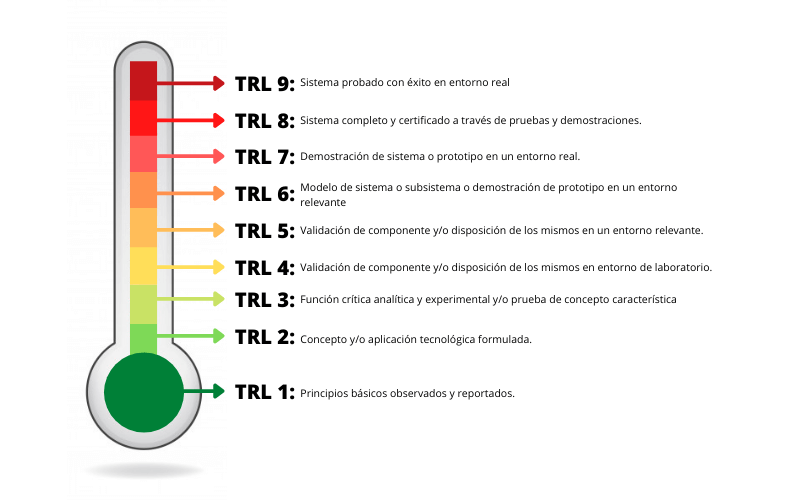
\includegraphics[width=0.8\linewidth]{Imagenes/COL.png}
  \caption{Extraida de Ayming\cite{o}}
  \label{fig:imagen2}
\end{figure}
\newpage


Considerando esto, la metodología de investigación planteada para el proyecto consistió en seguir etapas secuenciales para asegurar un proceso eficaz.
\\ \\
En primer lugar, se llevó a cabo una búsqueda bibliográfica con el fin de recopilar información pertinente acerca del desarrollo de las habilidades seleccionadas, los métodos educativos y las tecnologías de enseñanza disponibles. Esto con el objetivo de tener un conocimiento más sólido a la hora de diseñar el software. Cabe mencionar que, por consiguiente, durante esta etapa se seleccionaron las habilidades blandas a abordar.
\\ \\
Tras la finalización de la investigación, se procedió a la etapa de diseño y desarrollo del software para el aprendizaje y fortalecimiento de habilidades blandas a través de las diferentes tecnologías web y herramientas de desarrollo necesarias.
\\ \\
Después de la fase de desarrollo, se llevó a cabo la recolección de datos y evaluación utilizando diferentes medios, como encuestas y evaluaciones de desempeño. Esto permitió valorar la eficacia del software en el desarrollo de habilidades blandas. Una vez recopilada toda la información, se analizaron los datos para extraer conclusiones y generar recomendaciones de ajustes o posibles cambios futuros en la plataforma.


%Metodología de desarrollo de software
\section{Metodología de desarrollo de software}
Para el desarrollo de este proyecto se optó por una metodología ágil basada en la  necesidad de flexibilidad y eficiencia en el desarrollo del software básico para una tesis. Estos proyectos suelen enfrentar cambios en los requisitos y desafíos emergentes, por lo que requieren un enfoque adaptable que permite realizar ajustes constantes a lo largo del proceso.
\\ \\
La naturaleza volátil y cambiante de estos proyectos se encuentra en las metodologías ágiles como Scrum o Kanban. Este enfoque permite enfrentar la incertidumbre al enfocarse en principios como la simplicidad, la retroalimentación continua y la adaptación al cambio.
\\ \\
Una de las principales ventajas de Kanban radica en su enfoque visual y su capacidad para gestionar el flujo de trabajo de manera eficiente. Al utilizar columnas que representan etapas de trabajo y límites de trabajo en proceso (WIP), Kanban permite una visualización clara de las tareas en curso y ayuda a identificar cuellos de botella o áreas para mejorar la eficiencia. Esto facilita una rápida adaptación a los cambios en la demanda o prioridades del proyecto.
\\ \\
Mientras tanto Scrum se enfoca en la división del trabajo en iteraciones manejables, conocidas como sprints, facilita un proceso iterativo e incremental para la entrega del producto final, priorizando las necesidades esenciales y ajustando el enfoque conforme avanza el proyecto.
\\ \\
Para este proyecto, se ha optado por usar Scrumban, el cual fusiona las cualidades más destacadas de Scrum y Kanban. Combina la estructura orientada de Scrum con la flexibilidad y capacidad de adaptación de Kanban. 
\\ \\
“Scrumban se desarrolló inicialmente para ayudar a los equipos en su transición de Scrum a Kanban o viceversa. Si los equipos tienen más experiencia con una de las estrategias que con la otra, esta técnica les servirá para cambiar gradualmente de una metodología a otra. 
\\ \\
Si bien el motivo inicial por el que nació Scrumban fue para ayudar a que los equipos migren de un método al otro, en algunos casos, se descubrió que esta combinación de ambas estrategias resultaba beneficiosa.”\cite{p}
\\ \\
Además, al manejar cambios en los requisitos de manera efectiva, Scrumban permite realizar ajustes rápidos y eficaces incluso en etapas avanzadas del proyecto, lo que posibilita la constante mejora y optimización del software, minimizando así problemas futuros.

%Metodología de gestión de actividades
\section{Metodología de gestión de actividades}
Para la administración de las diferentes actividades y una visualización clara del flujo de trabajo se optó por el uso de tablero kanban puesto que esta herramienta, al igual que la metodología de desarrollo Scrumban , ofrece una mayor flexibilidad para adaptarse a las cambiantes necesidades del proyecto.

\section{Metodología de gamificacion}
Para una correcta aplicación de la gamificación se utilizaron una serie de técnicas mecánicas y dinámicas extraídas de dinámicas de juegos, las cuales incluyeron desafíos, misiones, logros y competiciones. Los desafíos representaron competiciones entre usuarios con el objetivo de obtener premios. Por otro lado, las misiones o retos implicaron resolver o superar objetivos planteados, ya sea individualmente o en equipo, promoviendo el logro personal y la satisfacción al alcanzarlos.
\\ \\
Los logros dentro de la gamificación educativa fueron resultados que contribuyeron a la superación individual y proporcionaron una sensación de satisfacción personal al cumplir metas específicas. La competición en este contexto implicó la búsqueda constante de mejorar y superar desafíos.
\\ \\
Es importante destacar que la esencia de la gamificación educativa no residió en la creación de juegos per se, sino en la implementación inteligente de sistemas como la puntuación, las recompensas y los objetivos que comúnmente se encuentran en los juegos. Estos elementos se utilizaron estratégicamente para fomentar la participación, el compromiso y el aprendizaje en entornos educativos.


%Progama de hitos
%\chapter{Progama de hitos}
%%Descomposición de los objetivos específicos

Para la formulación del calendario de actividades se utilizará un programa de hitos junto con el del planteo secuencial basándose en un sistema iterativa incremental donde la unidad mínima equivale a una semana de los 8 meses de duración del proyecto, cada actividad proviene de un objetivo específico.
\\ \\
\begin{longtable}{|p{8cm}|p{8cm}|}
        \hline
        \hline
        \rowcolor{naranja} \centering \textbf{Objetivo Específico} & \multicolumn{1}{|c|}{\textbf{Actividad}} \\ [1mm] 
        \multirow{4}{*}{\parbox{8cm}{\centering \textbf{Revisar la literatura enfocada en analizar las habilidades blandas mindset y fitness.}}} & 1.1 Revisar la literatura sobre las habilidades blandas seleccionadas 
\\ & 
1.2 Seleccionar artículos y estudios que aborden las habilidades blandas seleccionadas, así como los métodos educativos relacionados o su demanda en el mercado laboral
 \\ \hline

        \multirow{4}{*}{\parbox{8cm}{\centering \textbf{Desarrollar los módulos de mindset y fitness en la plataforma.}}}  & 2.1 Desarrollar los módulos de mindset y fitness. \\ & 2.2 Realizar pruebas y evaluaciones de los  módulos de la plataforma. \\ 
\hline


\multirow{4}{*}{\parbox{8cm}{\centering \textbf{Integrar características de gamificación en los módulos de mindset y fitness de la plataforma. }}} & 3.1 Identificar  los elementos de gamificación para los modulos de la plataforma. \\ & 3.2 Desarrollar los elementos de gamificación para los modulos de la plataforma.
 \\ \hline

 
        \multirow{4}{*}{\parbox{8cm}{\centering \textbf{Evaluar la usabilidad de los módulos mindset y fitness de la plataforma. }}} & 4.1. Evaluar utilizando diferentes medios, como encuestas y evaluaciones de desempeño \\ & 4.2. Realizar las conclusiones y recomendaciones de ajustes o posibles cambios futuros en los módulos. 
 \\ \hline

    \caption{Descomposición de objetivos específicos}
\end{longtable}


%Tabla programa de hitos
\begin{figure}[ht]
    \centering
    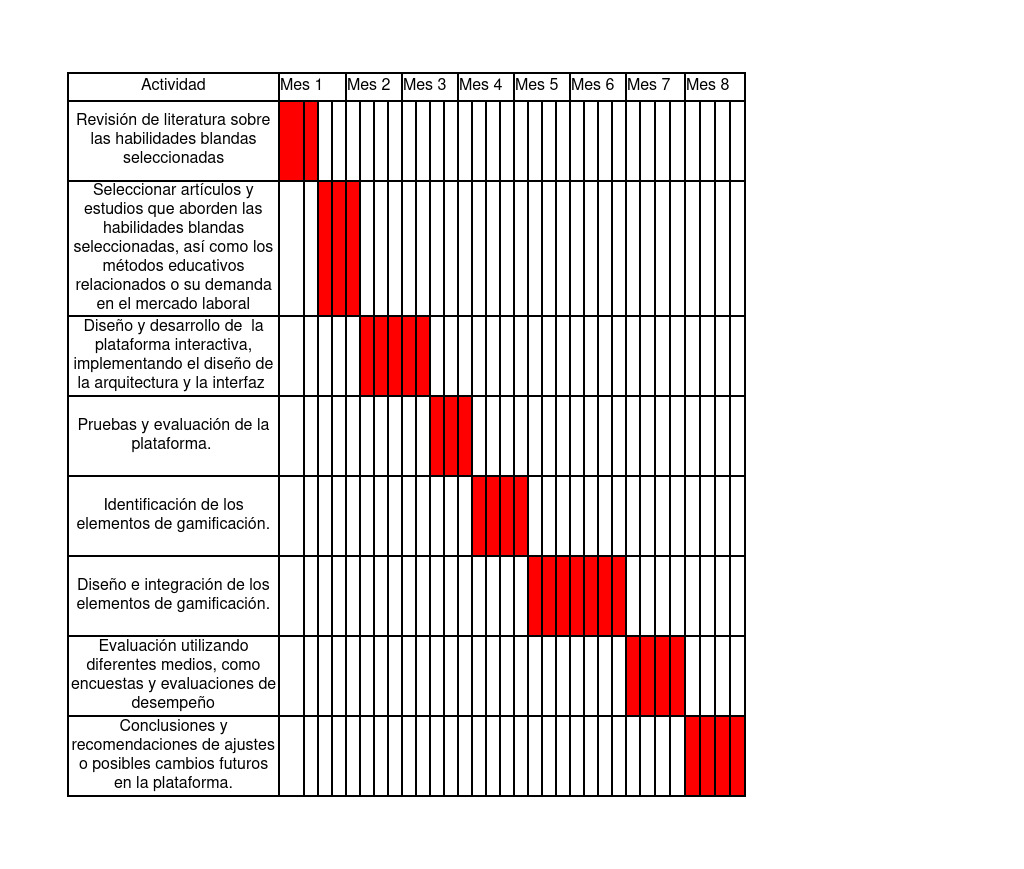
\includegraphics[width=25cm]{Imagenes/tabla-hitos.jpg}
    \caption{Programa de hitos}
\end{figure}

%Presupuesto
%\chapter{Presupuesto}
%\section{Presupuesto general}
\subsection{Gastos salariales}

La tabla en esta sección contiene los datos relevantes acerca del tiempo dedicado al proyecto, siguiendo las pautas establecidas por la según el artículo 11 del decreto 1295 del Ministerio de Educación MEN (2010) ”Un crédito académico equivale a cuarenta y ocho (48) horas de trabajo académico del estudiante, que comprende las horas con acompañamiento directo del docente y las horas de trabajo independiente que el estudiante debe dedicar a la realización de actividades de estudio, prácticas u otras que sean necesarias para alcanzar las metas de aprendizaje” y el artículo 12 del mismo decreto “teniendo en cuenta que una (1) hora con acompañamiento directo de docente supone dos (2) horas adicionales de trabajo independiente en programas de pregrado”.


\begin{table}[h]
    \centering
    
    \label{tab:resumen}
    \begin{tabular}{|l|r|}
        \hline
        \textbf{Número de créditos} & 9 \\
        \hline
        \textbf{Horas por crédito} & 48 \\
        \hline
        \textbf{Total de horas del trabajo investigativo} & 432 \\
        \hline
        \textbf{Horas disponibles del director} & 44 \\
        \hline
        \textbf{Horas totales del estudiante} & 388 \\
        \hline
    \end{tabular}
    \caption{Resumen de horas y créditos}
\end{table}

A continuación, la tabla presenta el cálculo del salario tanto para el profesor asociado como para el estudiante, basado en la tabla que detalla las horas correspondientes a cada uno:



\begin{table}[h]
    \centering
    \label{tab:costos}
    \begin{tabular}{|l|r|r|}
        \hline
        \textbf{Personal} & \textbf{Costo por hora} (pesos colombianos) & \textbf{Total} (pesos colombianos) \\
        \hline
        Estudiante & 7.250 & 2.813.000 \\
        Director trabajo de grado & 61.264 & 2.695.616 \\
        \hline
        \textbf{Total} & & 5.013.000 \\
        \hline
    \end{tabular}
    \caption{Costos salariales}
\end{table}
\newpage
\subsection{Gastos tecnológicos}
La depreciación del equipo de cómputo se calculará utilizando el método de depreciación en línea recta, considerando una vida útil de 60 meses. Este cálculo se basa en el valor inicial del equipo y su tiempo de vida útil para determinar la devaluación mensual del equipo. De esta manera, se obtiene un valor total para la duración del proyecto, que es de 8 meses


\begin{table}[h]
    \centering

    \begin{tabular}{|l|r|}
        \hline
        \textbf{Costo equipo de computo} & 1.500.000 \\
        \hline
        \textbf{Vida útil en meses} & 60 \\
        \hline
        \textbf{Desvalorización} & 25.000 \\
        \hline
        \textbf{Duración del proyecto en meses} & 8 \\
        \hline
        \textbf{Total (pesos colombianos)} & 200.000 \\
        \hline
    \end{tabular}
    \caption{Depreciación}
\end{table}

En la tabla siguiente se detalla el cálculo tanto para el costo del servicio eléctrico como para el internet durante el período necesario para el proyecto

\begin{table}[h]
    \centering
    \label{tab:detalles-proyecto}
    \begin{tabular}{|l|r|r|}
        \hline
        \textbf{Concepto} & \textbf{Costo mes} & \textbf{Valor(pesos colombianos)} \\
        \hline
        Internet & 65.000 & 520.000 \\
        Electricidad & 55.000 & 440.000 \\
        \hline
        \textbf{Total} & & 960.000 \\
        \hline
    \end{tabular}
    \caption{Detalles gasto electricidad e internet}
\end{table}

Proseguimos con la tabla del total de gastos tecnológicos:

\begin{table}[h]
    \centering
    
    \label{tab:gastos-tecnologicos}
    \begin{tabular}{|l|r|}
        \hline
        \textbf{Concepto} & \textbf{Valor (pesos colombianos)} \\
        \hline
        Equipo de computo & 960.000 \\
        Otros gastos tecnológicos & 266.667 \\
        \hline
        \textbf{Total} & 1.226.667 \\
        \hline
    \end{tabular}
    \caption{Detalles de gastos tecnológicos}
\end{table}
\newpage
\subsection{Presupuesto general total}
La tabla que sigue presenta el resumen del presupuesto total destinado al proyecto. Este presupuesto abarca los costos tecnológicos del hardware y los gastos de nómina del personal.


\begin{table}[h]
    \centering

    \label{tab:gastos}
    \begin{tabular}{|l|r|}
        \hline
        \textbf{Concepto} & \textbf{Valor (pesos colombianos)} \\
        \hline
        Gastos salariales & 5.508.616 \\
        Gastos tecnológicos & 1.226.667 \\
        \hline
        \textbf{Total} & 6.735.283 \\
        \hline
    \end{tabular}
    \caption{Gastos totales}
\end{table}



%literatura
\chapter{Revision de literatura}
 A continuación se presenta un estudio de la literatura que abarca libros y estudios relacionados con los temas principales, así como investigaciones sobre gamificación y proyectos similares. También se analizan los argumentos a favor y en contra, considerando los aspectos más relevantes para este caso de estudio en particular.
\\ \\

\begin{longtable}{|p{3cm}|p{6cm}|p{4cm}|p{4cm}|}
\hline
\textbf{Nombre}  & \textbf{Resumen} & \textbf{Pros} & \textbf{Contras} \\ 
\hline
\endfirsthead
\hline
\textbf{Nombre}  & \textbf{Resumen} & \textbf{Pros} & \textbf{Contras} \\ 
\hline
\endhead
\hline
\endfoot

Perspectivas en nutrición humana Escuela de Nutrición y Dietética
de la Universidad de Antioquia
Vol. 21, N.° 1\cite{1} & El documento ofrece una visión detallada sobre la importancia de la alimentación en la prevención de enfermedades crónicas no transmisibles, destacando la necesidad de promover el consumo diario de frutas y verduras. Asimismo, subraya la relevancia de adoptar un estilo de vida saludable, que integre la práctica regular de actividad física y la evitación de hábitos nocivos, como el consumo de tabaco y alcohol. & Una adecuada contextualización sobre las enfermedades provocadas por una alimentación deficiente, complementada con una sólida recopilación de datos.
 & Este es un documento breve de solo 6 páginas, que funciona más como una introducción que como un estudio exhaustivo.
 \\ 
\hline
Influencia del deporte y la actividad física en el estado de salud físico y mental\cite{2}
&
El artículo tiene como objetivo principal explorar y describir los beneficios que la práctica del deporte y la actividad física aportan al estado de salud, considerando tanto los aspectos físicos como mentales. Se destacan los efectos positivos de estas actividades en la salud, incluyendo la prevención de enfermedades crónicas, la mejora de la salud cardiovascular, y la reducción del estrés, la ansiedad y la depresión. Además, se subraya el fortalecimiento de habilidades cognitivas y sociales como otro de los beneficios significativos de la actividad deportiva. & El artículo presenta una revisión bibliográfica exhaustiva sobre la influencia del deporte y la actividad física en la salud física y mental, ofreciendo una visión clara de los beneficios asociados a la actividad física. Además, incluye una amplia variedad de fuentes confiables que respaldan sus hallazgos.
 & Dado que se basa en una revisión bibliográfica, el artículo incluye una gran cantidad de datos; sin embargo, no profundiza de manera extensiva en ningún tema específico.
 \\ 
\hline

Estrategias Gamificación aplicadas a la Educación y a la Salud\cite{3}
&
Este documento proporciona una exploración detallada de la integración de la gamificación en el ámbito educativo, con un enfoque particular en el diseño de interfaces interactivas. Se destaca la aplicación de elementos tanto individuales como sociales, con el objetivo de motivar a los estudiantes y potenciar su proceso de aprendizaje. Además, se centra en TANGO:H, una tecnología basada en el uso de Kinect de Microsoft©, que, a través de una cámara RGB y un sensor de profundidad, es capaz de reconocer el cuerpo humano.
 & La propuesta del artículo se diseñó y verificó a través de una clase de jóvenes, destacando las características de gamificación empleadas en el proceso.&El documento está demasiado centrado en TANGO:H
 \\ 
\hline
Gamificación en Educación Física\cite{4}
&
El documento resalta la importancia de implementar la gamificación en la educación física como una estrategia metodológica para enriquecer el proceso formativo de los estudiantes. Se subraya la necesidad de proporcionar experiencias motrices auténticas y significativas, alineadas con las necesidades actuales de los jóvenes, con el objetivo de fomentar un repertorio motriz amplio y diverso que tenga un impacto positivo en la salud. Además, el análisis se apoya en la revisión de 26 fuentes diferentes, lo que le otorga una sólida base teórica.
 & El documento demuestra el crecimiento significativo de la gamificación en diversos ámbitos educativos, destacando cómo esta tendencia ha transformado las prácticas pedagógicas. Se promueve una experiencia de aprendizaje que enriquece y fortalece el proceso formativo de los estudiantes, motivándolos a participar activamente y mejorando tanto su compromiso como su rendimiento académico.&Aunque es un buen recopilatorio, la información se limita a verificar el crecimiento del uso de la gamificación, lo que reduce su relevancia para este caso de estudio en particular. 
 \\ 
\hline
Play the Game: gamificación y hábitos saludables en educación física \cite{5}
&
El documento se enfoca en la implementación de una unidad didáctica gamificada denominada "Play The Game", llevada a cabo en centros educativos de Barcelona durante el primer trimestre del curso académico 2013-2014. Esta iniciativa se estructuró en torno a unidades didácticas diseñadas para fomentar la interacción entre el alumnado. La unidad comprendió un total de 12 sesiones de una hora cada una, y la muestra del estudio incluyó 3 profesores y 9 alumnos seleccionados a partir de proyectos previos.
 & El documento presenta 7 niveles de retos o juegos diseñados para el aprendizaje del alumnado, utilizando herramientas que abarcan desde formatos presenciales hasta virtuales. Además, se destacan metodologías efectivas que promueven el desarrollo individual de los estudiantes, potenciando tanto sus habilidades académicas como personales a través de la gamificación.
&Los datos analizados provienen de estudiantes preseleccionados, lo que podría influir en los resultados y limitar la generalización de los hallazgos. Además, el artículo tiene 9 años de antigüedad, lo que podría afectar la relevancia de sus conclusiones en el contexto educativo actual, dado que la tecnología y las metodologías han evolucionado considerablemente desde entonces.
 \\ 
\hline
How to win friends and influence people\cite{6}
&
El libro se enfoca en técnicas esenciales para interactuar de manera efectiva con los demás. Dale Carnegie subraya la importancia de demostrar un interés genuino en las personas, practicar una escucha activa y ofrecer elogios sinceros. También propone estrategias clave para ganar la simpatía de los demás, tales como recordar y utilizar el nombre de la persona, conversar en función de sus intereses y evitar hacer críticas directas. Estas técnicas buscan mejorar las relaciones interpersonales y fomentar una comunicación más efectiva y positiva.
 & El libro ofrece diversas pautas sobre cómo influir en otras personas mediante el autodesarrollo y la influencia en uno mismo. Destaca la importancia de mejorar nuestras propias habilidades interpersonales y actitudes, como clave para impactar positivamente en los demás. A través de la autogestión y el control emocional, el autor sugiere que es posible ejercer una influencia más efectiva sobre quienes nos rodean.&La primera mitad del libro se enfoca en las interacciones con otras personas, mientras que la segunda mitad resulta ser la más útil para este caso de estudio. 
 \\ 
\hline
Think and Grow Rich \cite{7}
&
"Piense y Hágase Rico" de Napoleón Hill es una obra que examina cómo los pensamientos influyen en la creación de riqueza y éxito personal. El autor destaca el poder de la autosugestión, la fe y una planificación meticulosa como elementos clave para alcanzar el éxito. Asimismo, presenta diversas herramientas y estrategias diseñadas para convertir los pensamientos en acciones concretas que faciliten el logro de las metas propuestas.
 & El libro ofrece valiosos consejos enfocados en la autosuperación y la motivación personal, proporcionando estrategias prácticas para desarrollar una mentalidad positiva y proactiva.&El libro no se basa en fundamentos científicos, sino que recurre a enfoques empíricos, apoyándose en experiencias personales y ejemplos anecdóticos para sustentar sus ideas. 
 \\ 
\hline
Psycho-Cybernetics \cite{8}
&
"Psycho-Cybernetics", es un libro de autoayuda escrito por Maxwell Maltz en 1960, que emplea aspectos psicológicos del ser humano para promover el mejoramiento de la autoimagen. Maltz sostiene que una imagen propia positiva es clave para alcanzar una vida más exitosa y satisfactoria, ofreciendo herramientas y estrategias para reprogramar la mente y modificar patrones de pensamiento que impiden el crecimiento personal.
 & El libro fue avalado y ampliamente elogiado por diversos autores, consolidando su reputación como una obra influyente en el ámbito del desarrollo personal. Además, incluye múltiples anécdotas que, junto con las actualizaciones presentes en la versión de 2002, lo convierten en un libro completo y enriquecedor, proporcionando una visión integral del proceso de mejora de la autoimagen.&Aunque es un libro relativamente antiguo, su enfoque en la autopercepción lo mantiene plenamente vigente en nuestro contexto actual. Los principios que aborda, relacionados con la autoimagen y el desarrollo personal, siguen siendo relevantes y aplicables, independientemente del paso del tiempo. 
 \\ 
\hline
Atlas Shrugged \cite{9}
&
La rebelión de Atlas es una novela que narra una rebelión ficticia de grandes empresarios contra los políticos y el gobierno de los Estados Unidos. La obra retrata a los empresarios vanguardistas como el "Atlas" (el dios griego que sostiene el mundo), simbolizando su carga de responsabilidad y sus luchas en una sociedad que depende de ellos desesperadamente, pero que al mismo tiempo los oprime y desprecia. La novela explora los desafíos y sacrificios que enfrentan en un mundo que necesita su innovación y liderazgo para prosperar.
 & La novela fomenta eficazmente una actitud positiva y la autosugestión, destacando la importancia de la determinación y el poder personal frente a las adversidades.&La novela es considerablemente extensa, con un total de 1,058 páginas, lo que la convierte en una lectura densa. Además, cuenta con una antigüedad significativa, lo que refleja su contexto histórico y filosófico. 
 \\ 
\hline
Del gimnasio al ocio-salud \cite{10}
&
El documento ofrece información valiosa sobre la relación entre el ocio, la gestión deportiva y el turismo, subrayando la importancia de desarrollar experiencias emocionantes y satisfactorias para los consumidores. También destaca la evolución de los centros dedicados a la actividad deportiva y a la salud, evidenciando cómo han adaptado sus servicios para satisfacer las necesidades y expectativas de los usuarios por el paso del tiempo.
 & 
Proporciona información relevante sobre los centros deportivos y sus transformaciones a lo largo de la historia, contextualizando adecuadamente su importancia en el ocio y la cultura general. &El artículo fue publicado en 2007 y, aunque busca contextualizar los centros deportivos hasta la actualidad, es probable que se quede algo corto en su análisis. 
 \\ 
\hline
Desarrollo de Prototipo de sistema de recomendación para rutina de ejercicio cardiovascular\cite{11}
&
El trabajo de grado de Paola Andrea Lenis Franco se enfoca en el desarrollo de un prototipo de sistema de recomendación para rutinas de ejercicio cardiovascular. Este sistema, diseñado a través de plataformas web, permite a los usuarios registrar información sobre enfermedades cardiovasculares, lo que facilita la creación de rutinas personalizadas y seguras.
 & 
El prototipo permite la adición de nuevas enfermedades en la plataforma web, lo que asegura su actualización continua y relevancia a lo largo del tiempo. &Es necesario reevaluar la base de datos y el código de manera manual al añadir nuevas enfermedades si se desean incluir rutinas específicas para estas.  
 \\ 
\hline
Prototipo de sistema de recomendación para el apoyo a futbolistas amateur en el desarrollo de su entrenamiento deportivo de manera individual\cite{12}
&
El trabajo se centra en el desarrollo de una aplicación para un sistema de recomendación de entrenamiento deportivo individualizado, que se fundamenta en el estado físico y la capacidad deportiva de cada persona.
 & 
La usabilidad de la aplicación fue evaluada como excelente, lo que indica una experiencia positiva para los usuarios. Los inconvenientes identificados durante el primer despliegue del prototipo fueron cuidadosamente abordados y corregidos. &La aplicación tuvo reseñas mixtas pero es normal puesto que es un prototipo.  
 \\ 
\hline
Desarrollo de prototipo de aplicación móvil para entrenamientos fisicos\cite{13}
&
El trabajo se centra en el desarrollo de una aplicacion  para recomendación de entrenamientos fisicos mediante la calificacion de ciertos ejercicios por el usuario, creando a su vez un entorno mas comodo y perzonalizado para cada usuario
 & 
La aplicación incluye información relevante sobre el módulo de recomendación, destacando el uso de modelos de clasificación como One Hot Encoding y Label Encoding.Los resultados obtenidos de la aplicación cumplieron con las expectativas, lo que sugiere que el sistema de recomendación es eficiente y útil para los usuarios en la personalización de sus entrenamientos deportivos. & 
\\
\hline
Meditaciones de marco aurelio\cite{14}
&
El libro presenta las diversas meditaciones del emperador romano Marco Aurelio, en las que ofrece consejos sobre el ser, fundamentados principalmente en principios estoicos. Estas reflexiones están organizadas en 12 libros breves, cada uno de los cuales aborda diferentes aspectos de la vida, la virtud y la autoconciencia.
 & 
El libro aborda de manera sobresaliente cómo debe ser la conducta ante diversas situaciones, principalmente en la vida cotidiana. La información está estructurada en secciones, que a su vez se dividen en consejos simples y complejos, lo que permite que cada punto sea relevante por sí mismo, sin necesidad de consultar el resto del contenido. & Dado que se trata de una traducción, es recomendable releer el texto para asegurar una correcta comprensión de los conceptos y matices presentados. 
\\
\hline
Sindrome del tunel carpiano\cite{15}
&
La revisión bibliográfica ofrece un análisis introductorio sobre el síndrome del túnel carpiano, incluyendo diversos aspectos como su diagnóstico y tratamientos disponibles. Además, se proporciona información relevante que permite comprender mejor esta condición, sus síntomas y la efectividad de las intervenciones propuestas.
 & 
El documento es una excelente fuente para contextualizarse sobre el síndrome del túnel carpiano, proporcionando datos relevantes y útiles que ayudan a entender mejor esta condición y sus implicaciones. & 
\\
\hline
Terapia manual en el síndrome del túnel carpiano.\cite{16}
&
El documento es una revisión que evalúa la efectividad de la terapia manual, centrándose en las técnicas de neurodinamia y masoterapia, en el manejo clínico del síndrome del túnel carpiano (STC).
 & 
El documento detalla las técnicas e instrumentos utilizados en la evaluación, así como la catalogación de sus resultados. Se encontraron resultados satisfactorios tanto al emplear las técnicas de masoterapia y neurodinamia de manera individual como al combinarlas, lo que sugiere que estas intervenciones pueden ser efectivas en el tratamiento del síndrome del túnel carpiano. & Se requieren estudios adicionales sobre el síndrome del túnel carpiano (STC) en sus formas moderada y severa, con un mayor número de pacientes, para validar los resultados obtenidos y establecer conclusiones más robustas sobre la efectividad de las intervenciones terapéuticas.
\\
\hline
Efectividad de la movilización neurodinámica en el dolor y funcionalidad en sujetos con síndrome del túnel carpiano: revisión sistemática.\cite{17}
&
El documento es una revisión de literatura que examina la efectividad de la técnica de movilización neurodinámica en pacientes diagnosticados con síndrome del túnel carpiano.
 & 
De los cuatro estudios seleccionados, que inicialmente sumaban 63, se contó con la participación de 261 pacientes, lo que proporciona una muestra significativa para la obtención de resultados. El estudio concluyó con evidencia notable y de nivel moderado sobre la efectividad del método. Este enfoque se diseñó considerando tanto los costos como las preferencias del paciente; al tratarse de un grupo de técnicas, puede ofrecer una solución eficaz a un costo prácticamente nulo. & A diferencia de las herramientas o procedimientos quirúrgicos, las técnicas mencionadas pueden no tener el mismo impacto, ya que su efectividad puede depender de la disposición y el compromiso del paciente.
\\
\hline
Videojuegos, práctica de actividad física, obesidad y hábitos sedentarios en escolares de entre 10 y 12 años de la provincia de Granada.\cite{18}
&
La investigación examina el sobrepeso y la actividad física en una muestra de 261 niños y niñas de entre 10 y 12 años. Además, se analiza la influencia de ciertos hábitos, incluyendo el uso de videojuegos, en el estado de salud de los participantes.
 & 
El documento presenta de manera clara y efectiva los resultados obtenidos en los diferentes tipos de estudios.
 & Las conclusiones del estudio resultaron ser contrarias al objetivo inicial, evidenciando que el 55,6 por ciento de los estudiantes se encontraba en un estado de bajo peso, un hallazgo que se destacó adecuadamente en la sección de conclusiones.
\\
\hline
Motivación del estudiante y los entornos virtuales de aprendizaje (Educación a distancia y ruralidad).\cite{19}
&
El documento se centra en un análisis de las diversas plataformas educativas, evaluando su utilidad y eficacia en relación con los estudiantes.
 & 
El análisis proporciona una excelente contextualización sobre el tema, destacando los posibles problemas asociados con el uso de estas plataformas y ofreciendo orientación sobre cómo utilizarlas de manera efectiva.
 & Dado que se trata de un análisis, la información proporcionada puede ser limitada, lo que podría hacer que resulte insuficiente como material final para este proyecto.
\\
\hline
Experiencias de gamificación en aulas.\cite{20}
&
El libro "Experiencias de gamificación en aulas"  como su título indica, presenta diversas experiencias de educadores en la implementación de la gamificación, así como las estrategias empleadas por ellos. Cabe destacar que esta es la segunda edición del libro.

 & 
El libro ofrece una sólida contextualización del tema, junto con una descripción detallada de siete juegos específicos y las estrategias necesarias para implementarlos de manera efectiva en el aula.
 & 
\\
\hline
Gamificación Como Estrategia De Motivación En La Plataforma Virtual De La Educación Superior Presencial.\cite{21}
&
El documento tiene como objetivo desarrollar una propuesta de gamificación mediante la recolección de datos a través de encuestas. Además, busca proporcionar información relevante que sirva para futuras aplicaciones de la gamificación en entornos educativos.
 & 
El documento recopila y analiza una extensa cantidad de información que, independientemente de su aplicación en gamificación, puede resultar de gran utilidad para diversos propósitos.
 & El documento no pone en práctica el modelo de gamificación, lo que sugiere la necesidad de un estudio futuro para validar los resultados y la efectividad de la propuesta.
\\
\hline
La plataforma kahoot influye en la motivación durante la evaluación en los estudiantes de cuarto grado de primaria de la institución educativa nueva juventud de santa rita de siguas – Arequipa, 2020.\cite{22}
&
El documento se centra en un estudio que aborda la plataforma Kahoot desde dos enfoques. El primero es un análisis conceptual que examina la plataforma y su uso como herramienta de gamificación. El segundo enfoque se basa en una investigación sobre la opinión de los educandos que utilizaron Kahoot, a través de encuestas, para comprender su percepción de la plataforma.
 & 
El documento proporciona una visión clara de la percepción que tienen los educandos sobre una herramienta ampliamente reconocida en el ámbito de la educación gamificada. 
 & Dado que los participantes del estudio son educandos de poca edad, es posible que sus opiniones estén sesgadas a favor de la herramienta. 
\\
\hline
La resiliencia en la educación, la escuela y la vida.\cite{23}
&
El documento habla de la resilencia, utilidad e importancia en la eduacion y vida dia dia de las personas, ademas de ciertas caracteriticas que influyen en su desarrollo.
 & 
El documento, aunque es breve, es conciso y explica de manera efectiva el concepto de resiliencia y su relevancia. Proporciona una visión clara de cómo la resiliencia puede influir positivamente en la vida de las personas, especialmente en el contexto educativo.
 & El documento funciona más como un análisis introductorio sobre la resiliencia que como un desarrollo profundo del tema.Por lo tanto, podría resultar ineficaz para el contexto y los objetivos de este proyecto. 
\\
\hline
Resiliencia: Impacto Positivo En La Salud Física Y Mental\cite{24}
&
El documento analiza el impacto positivo de la resiliencia en la salud física y mental, destacando cómo la capacidad de adaptarse a situaciones adversas contribuye al bienestar general. Se enfatiza que desarrollar habilidades resilientes puede reducir problemas de salud mental y físico.
 & 
Es un buen documento para contextualizar la resiliencia y sus impactos en las personas, proporcionando información valiosa sobre su importancia en el bienestar general.
 &  
\\
\hline
La Sociedad del Espectáculo\cite{25}
&
Se trata de un libro filosófico-político que aborda el concepto del espectáculo no solo como entretenimiento, sino como una simulación de la realidad objetiva. El autor se refiere al espectáculo como la interacción entre dos personas a través de una imagen, en lugar de una conexión directa con la realidad, enfatizando la apariencia como un sustituto de la verdad.
 & 
El libro ofrece una perspectiva alternativa sobre la realidad y propone un cambio de paradigma en la forma de percibir el mundo. A través de su análisis, busca inspirar a los lectores a cuestionar las apariencias y a reflexionar sobre la autenticidad de sus experiencias.
 &  
\\
\hline
Soft Skills: The software developer's life manual\cite{26}
&
El libro "Soft Skills" es un manual dirigido a desarrolladores de software que ofrece técnicas y prácticas centradas en el desarrollo de habilidades blandas. Abarca temas como relaciones interpersonales, gestión financiera y aspectos relevantes para el proyecto, como el mindset y el fitness.
 & 
El libro contiene información importante tanto de fitness como de mindset, Además de  contar con diferentes ejemplos a tomar en cuenta sobre las habilidades blandas

 &  
\\
\hline
\caption{Tabla de estudios y proyectos relacionados}
\label{tab:estudios}
\end{longtable}


Para el desarrollo de este proyecto, se seleccionaron los siguientes trabajos:  
``Desarrollo de prototipo de aplicación móvil para entrenamientos físicos``,  
``Meditaciones de Marco Aurelio``,  
``Experiencias de gamificación en aulas``,  
``Soft Skills: The Software Developer's Life Manual`` y  
``La Sociedad del Espectáculo``.  
\\ \\
La selección se realizó considerando los pros y contras descritos en la tabla anterior, así como la estructura requerida para obtener información relevante sobre la gestión de proyectos que incorporan gamificación.
\\ \\
Además, también se tomaron en cuenta factores de mayor utilidad para este caso de estudio. Por ejemplo,  
``Desarrollo de prototipo de aplicación móvil para entrenamientos físicos`` y  
``Experiencias de gamificación en aulas`` presentaron ejemplos de gamificación.  
El primero menciona métodos para animar a un usuario desde el punto de vista del mindset, mientras que el segundo se enfoca en mejorar un aspecto físico como el fitness. Ambos trabajos presentaron resultados satisfactorios en el contexto de la gamificación, haciéndolos muy útiles por su experiencia para este proyecto.
\\ \\
En el caso de  
``Meditaciones de Marco Aurelio`` y  
``La Sociedad del Espectáculo``,  
ambos libros, a través de la experiencia de sus autores, analizan el *psique* humano y cómo, al cambiar el método de pensamiento, se puede afectar el entorno que rodea al individuo.  
El primero plantea cómo actuar para cambiar el mundo, mientras que el segundo propone modificar el análisis para verlo desde una perspectiva diferente.
\\ \\
Por último, el libro ``Soft Skills: The Software Developer’s Life Manual`` se considera la principal fuente de información sobre las habilidades blandas, ya que se enfoca en diversas experiencias tanto académicas como laborales, con gran utilidad para este caso de estudio.
\\ \\
Posteriormente, se decidió realizar un análisis detallado para determinar cómo abordar las habilidades blandas a través de la gamificación. En el caso de la categoría de fitness, se optó por enfocarse en dos problemas principales que afectan con frecuencia a los ingenieros en sistemas: la prevención del síndrome del túnel carpiano y la mejora de la postura, especialmente en áreas como el coxis, que suelen causar molestias debido a largas horas frente al ordenador.
\\ \\
Para la categoría de mindset, se decidió centrarse en algunas de las habilidades clave para los ingenieros en sistemas, muchas de ellas mencionadas en el libro "Soft Skills: The Software Developer's Life Manual" y otras identificadas como importantes para las personas en general, como en "Meditaciones de Marco Aurelio". Las habilidades seleccionadas incluyen la resiliencia, el pensamiento lógico y el aprendizaje continuo . A partir de estas, se realizó un análisis específico para determinar cómo abordarlas de manera efectiva. Cada habilidad fue subdividida según los desafíos comunes que enfrenta un ingeniero en sistemas, ya sea en su contratación o en su vida académica, y las competencias necesarias para superar dichos obstáculos.
\\ \\
A continuación, se presentan las tablas que detallan este análisis:


\begin{longtable}{|p{6cm}|p{3cm}|p{8cm}|}
\hline
\textbf{Problema}  & \textbf{Habilidad} & \textbf{Significado}  \\ 
\hline
\endfirsthead
\hline
\textbf{Problema}  & \textbf{Habilidad} & \textbf{Significado}  \\ 
\hline
\endhead
\hline
\endfoot

Dificultades al autoevaluarse como candidato potencial para una empresa & Autoconsciencia & Se refiere a la capacidad de una persona para estar consciente de sí misma,en términos de su propia existencia como de sus pensamientos, emociones, características y capacidades.

 \\ 
 \hline
Mala toma de decisiones bajo presión
&
Autocontrol
 & 
El autocontrol se refiere a la capacidad de una persona para regular y gestionar sus propias emociones, pensamientos y comportamientos en situaciones diversas. 

\\ 
 \hline
Tendencia a tener un ambiente negativo
&
Optimismo
 & 
Es una actitud mental positiva que implica esperar lo mejor en cualquier situación. 

\\ 
\hline
Las tareas tienden a ser muy diversas entre si
&
Adaptabilidad
 & 
La adaptabilidad se refiere a la capacidad de una persona para ajustarse y prosperar en entornos cambiantes o situaciones nuevas. Implica ser flexible, receptivo y capaz de cambiar de enfoque o estrategia según sea necesario en el caso de estudio o programa
\\ 
\hline

Se tiende a tener un pensamiento muy centrado en las normas por lo que ciertos problemas no tienen solución

&
Creatividad
 & 
La creatividad es la capacidad de generar ideas originales y únicas, así como de encontrar soluciones innovadoras a problemas o situaciones.


\\
\hline
Se tiende a tener una gran carga de trabajo al no completar un objetivo aunque sea en equipo
&
Gestión del estrés
 & 
La gestión del estrés se refiere a las estrategias y técnicas utilizadas para manejar y reducir los niveles de estrés en la vida diaria.

\\
\hline
Al generar una serie de soluciones no se pueden a aplicar todas

&
 Toma de decisiones & 
La toma de decisiones es el proceso mediante el cual una persona elige entre diferentes opciones disponibles con el fin de resolver un problema o alcanzar un objetivo .

\\
\hline
Se tiende a trabajar con diferentes tipos de codigo
&
Flexibilidad cognitiva
 & 
La flexibilidad cognitiva es la capacidad de adaptar y cambiar los procesos mentales y cognitivos en respuesta a nuevas situaciones, desafíos o información.
\\
\hline
El código tiende a fallar y genera estrés

&
Persistencia & 
La persistencia se refiere a la capacidad de una persona para continuar esforzándose y trabajando hacia un objetivo a pesar de los desafíos, obstáculos o fracasos que puedan surgir en el camino.

\\
\hline
Comúnmente se necesita cambiar de empleo

&
Habilidades sociales

 & 
Las habilidades sociales se refieren a las capacidades que una persona posee para interactuar de manera efectiva y apropiada con los demás en diversos contextos sociales.

\\
\hline
 Se tiende a menospreciarse a sí mismo como programador por ciertos puestos de trabajo sin experiencia

&
Autoaceptación
 & 
La autoaceptación es la capacidad de aceptarse a uno mismo tal como uno es, con todas las fortalezas, debilidades, imperfecciones y características únicas. 



\\
\hline

\caption{Tabla de subhabilidades sobre la reciliencia}
\label{tab:estudios}
\end{longtable}


\begin{longtable}{|p{6cm}|p{3cm}|p{8cm}|}
\hline
\textbf{Problema}  & \textbf{Habilidad} & \textbf{Significado}  \\ 
\hline
\endfirsthead
\hline
\textbf{Problema}  & \textbf{Habilidad} & \textbf{Significado}  \\ 
\hline
\endhead
\hline
\endfoot

Se tiene un volumen muy alto de datos.&  Análisis de datos & El análisis de datos es el proceso de examinar, limpiar, transformar y modelar datos con el objetivo de descubrir patrones, tendencias, relaciones o insights significativos que puedan utilizarse para tomar decisiones informadas o realizar predicciones. 

 \\ 
 \hline
Los datos parecen tener similitud
&
Interpretación de patrones
 & 
La interpretación de patrones se refiere al proceso de analizar datos, observar regularidades o tendencias recurrentes y extraer significado o conocimiento de ellos.

\\ 
 \hline
El programa es muy complejo y nesecita simplificarse &
Abstracción
 & 
La abstracción es un concepto que se refiere a la capacidad de representar o entender un objeto, idea o concepto de una manera simplificada, general o más abstracta, que elimina detalles innecesarios o irrelevantes. 

\\ 
\hline
Problemas matemáticos
&
Resolución de problemas lógicos
 & 
La resolución de problemas lógicos implica la aplicación de principios y reglas de la lógica para encontrar soluciones a situaciones que requieren razonamiento y análisis.
\\ 
\hline

Se encontró un problema pero muchas posibles causas

&
Pensamiento crítico & 
El pensamiento crítico es una habilidad mental que implica analizar de manera objetiva y racional la información, evidencia o argumentos presentados, con el fin de llegar a conclusiones fundamentadas y tomar decisiones informadas. 


\\
\hline
El cliente pidió un programa de forma muy abierta


&
Pensamiento analítico & 
El pensamiento analítico es una habilidad cognitiva que implica descomponer información compleja en partes más pequeñas y comprensibles para comprender mejor su estructura, relaciones y componentes individuales.
\\
\hline
Se solicita la evaluación de un programa mediante un problema


&
  Pensamiento sistemático & 
El pensamiento sistemático es una habilidad cognitiva que implica abordar problemas o situaciones de manera metódica y estructurada, siguiendo un enfoque ordenado y lógico. 

\\
\hline
El cliente pidió un programa de forma muy completa pero solicitó extras

&
Inducción y su razonamiento & 
La inducción es un proceso de razonamiento en el cual se llega a una conclusión general a partir de observaciones específicas o evidencias particulares. 

\\
\hline

\caption{Tabla de subhabilidades sobre el  pensamiento lógico}
\label{tab:estudios}
\end{longtable}


\begin{longtable}{|p{6cm}|p{3cm}|p{8cm}|}
\hline
\textbf{Problema}  & \textbf{Habilidad} & \textbf{Significado}  \\ 
\hline
\endfirsthead
\hline
\textbf{Problema}  & \textbf{Habilidad} & \textbf{Significado}  \\ 
\hline
\endhead
\hline
\endfoot

Se solicita que el empleado se adecue a un programa &  Curiosidad&La curiosidad es un rasgo fundamental del ser humano que impulsa el deseo de explorar, descubrir y aprender sobre el mundo que nos rodea.

 \\ 
 \hline
Se necesita un mayor sueldo que requiere mayor educación

&
Búsqueda de conocimiento
 & 
La búsqueda de conocimiento es el proceso activo y continuo de adquirir información, comprender conceptos y explorar nuevas ideas con el objetivo de ampliar la comprensión del mundo y enriquecer el pensamiento.

\\ 
 \hline
Los lenguajes de programación tienden a cambiar rápidamente

 &
 Autodidactismo
 & 
El autodidactismo es un enfoque de aprendizaje en el que una persona adquiere conocimientos y habilidades de manera independiente, sin la guía directa de un maestro o instructor formal.



\\ 
\hline
Se requiere adecuarse prontamente a un trabajo

&
Experimentación, Reflexión y Retroalimentación

 & 
La experimentación proporciona experiencias concretas que pueden ser reflexionadas y analizadas para extraer lecciones y aprendizajes significativos. La retroalimentación proporciona información adicional que ayuda a enriquecer la reflexión y a guiar futuras acciones y experimentos.

\\ 
\hline


\caption{Tabla de subhabilidades sobre el  aprendizaje continuo}
\label{tab:estudios}
\end{longtable}

Después de analizar las tablas, se destacaron nueve sub-habilidades, divididas en tres para cada área. En el caso de la resiliencia, las sub-habilidades son: autocontrol, adaptabilidad y toma de decisiones. Para el pensamiento lógico, se identificaron la interpretación de patrones, la abstracción y el pensamiento crítico. Finalmente, en el aprendizaje continuo se resaltaron: curiosidad, búsqueda de conocimiento y autodidactismo.
\\
En el caso de autocontrol y toma de decisiones, estas sub-habilidades fueron seleccionadas porque son cruciales para ayudar a seleccionar soluciones óptimas en tiempo limitado y bajo presión. Por otro lado, la adaptabilidad fue elegida debido a que se considera una habilidad indispensable para cualquier ingeniero en sistemas, independientemente de su área de vocación.
\\
La interpretación de patrones, la abstracción y el pensamiento crítico representan, probablemente, de la mejor forma lo que significa ser un ingeniero en sistemas capaz. Por ello, su inclusión en los ámbitos de este proyecto se considera fundamental.
\\
Por último, la curiosidad, la búsqueda de conocimiento y el autodidactismo representan los aspectos más esenciales que debe tener un estudiante, no solo para su desarrollo durante el periodo universitario, sino también para enfrentarse con éxito al mundo laboral.








%desarrollo
\chapter{Desarrollo de los modulos}

\section{Desarrollo de los modulos}
En este capítulo se destacaron las partes más importantes del desarrollo de los módulos, enfocándonos en los aspectos clave que contribuyeron a su implementación exitosa y al cumplimiento de los objetivos propuestos.
Para el desarrollo de los módulos, es importante destacar que, al igual que la plataforma que los contiene, se utilizó React, una biblioteca de código abierto basada en JavaScript, la cual facilita la creación de interfaces de usuario dinámicas y eficientes. A continuación, se detallan los elementos utilizados en la creación de los dos módulos de fitness: uno enfocado en ayudar a mantener una buena postura de la espalda y otro en la prevención del síndrome del túnel carpiano. También se describe el módulo de mindset, diseñado para fortalecer habilidades como la interpretación de patrones, el autocontrol, la adaptabilidad, entre otras. Todo lo desarrollado se encuentra disponible en https://github.com/azcaratejuan/soft-skills-plataform \subsection{Modulo fitness}
\subsubsection{Modulo fitness: Ejercicios para el tunel carpiano}
Para el desarrollo de la primera gamificacion especificamente para prevenir el síndrome del túnel carpiano, se decidió utilizar tecnologías capaces de reconocer las poses de las manos. En este caso, se empleó TensorFlow de Google, específicamente el modelo Handpose, el cual identifica 21 puntos clave en la mano, incluyendo todas las articulaciones de los dedos y las puntas de los mismos. Estos puntos se utilizan para calcular poses específicas mediante el uso de inteligencia artificial.
\\
Como consecuencia, se diseñó un juego que aprovecha diferentes posiciones de las manos para prevenir el síndrome del túnel carpiano, siguiendo las recomendaciones descritas en el documento "Síndrome del Túnel Carpiano: Protocolo de Tratamiento Conservador"\cite{14_1}. Las posiciones de la mano se usan en el juego para realizar acciones como subir, bajar o esquivar obstáculos, tal como se demuestra en la siguiente imagen:
\begin{figure}[H]
  \centering
  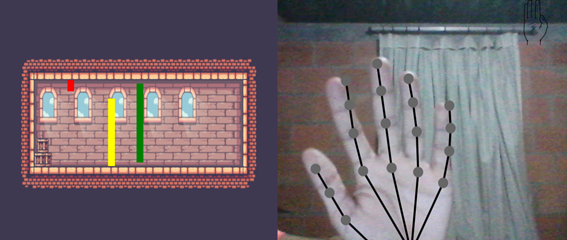
\includegraphics[width=0.6\linewidth]{Imagenes/Fitness1.png}
  \caption{Módulo fitness, imagen de muestra de gamificación sobre el túnel carpiano. Elaboración propia}
  \label{fig:imagen1fitness}
\end{figure}


Posteriormente, se añadieron otros elementos gamificados, como un contador que mide el tiempo que el jugador ha resistido, con el objetivo de incentivar al usuario a alcanzar el mayor puntaje posible. Estos elementos añaden dinamismo y motivación,Ademas se agregaron los botones para iniciar/pausar  y uno para reiniciar el juego como se ilustra en la siguiente imagen:

\begin{figure}[H]
  \centering
  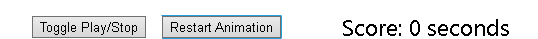
\includegraphics[width=0.6\linewidth]{Imagenes/Fitness2.png}
  \caption{Módulo fitness, imagen de muestra sobre botones y elemento puntuación de gamificación sobre el túnel carpiano. Elaboración propia}
  \label{fig:imagen2fitness}
\end{figure}

Finalmente, se añadió una imagen inicial con instrucciones para que el jugador comprendiera tanto los botones como las posiciones que deberá usar durante el juego:
\begin{figure}[H]
  \centering
  \includegraphics[width=0.5\linewidth]{Imagenes/tutorial-muñeca.png}
  \caption{Módulo fitness, imagen de las instrucciones sobre gamificación del túnel carpiano. Elaboración propia}
  \label{fig:imagen3fitness}
\end{figure}



\subsubsection{Modulo fitness: Ejercicios para la corrección de la mala postura de la espalda}
Para el desarrollo de la segunda parte del módulo de fitness, se decidió utilizar tecnologías capaces de detectar poses en este caso también de Google llamada Media-Pipe en su apartado hand landmarks. El cual identifica la posición de las manos en pantalla mediante inteligencia artificial.
\\
A partir de esta tecnología, se decidió desarrollar un juego enfocado en estiramientos para la espalda. Aprovechando la detección de la posición de las manos, el juego está diseñado para promover estiramientos básicos, incentivando al usuario a cambiar la posición de las manos de manera constante. Se emplean varias posiciones predefinidas, que guían al usuario a realizar los movimientos correctos para mejorar su postura y prevenir dolores asociados a la mala alineación de la espalda. A continuación, se muestran las posiciones utilizadas:
\begin{figure}[H]
  \centering
  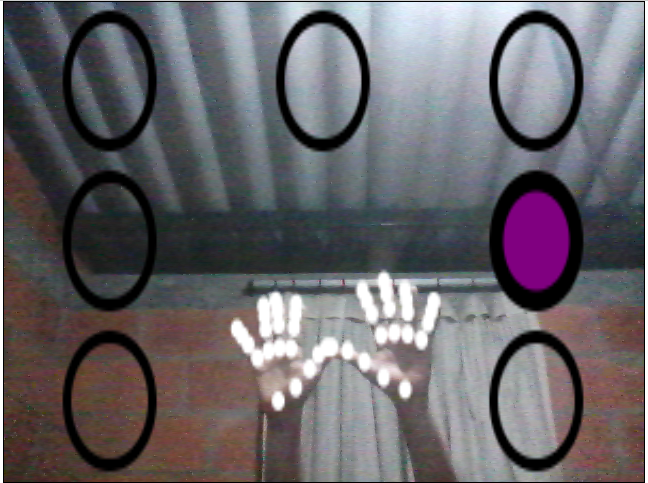
\includegraphics[width=0.6\linewidth]{Imagenes/Fitness3.png}
  \caption{Módulo fitness, imagen de muestra sobre gamificación para la corrección de mala postura en la espalda. Elaboración propia}
  \label{fig:imagen4fitness}
\end{figure}


Como resultado, se implementó un sistema en el que, al seleccionar una canción, se muestra una serie de movimientos que el usuario debe seguir, complementado con la reproducción de música para hacer la experiencia más agradable. Al igual que en el módulo anterior, se añadieron elementos gamificados, como un contador que mide la cantidad de movimientos correctos realizados por el usuario, incentivando así a alcanzar el mayor puntaje posible. Además, se incorporaron botones de iniciar y pausar para una mejor interacción, como se muestra en la siguiente imagen:


\begin{figure}[H]
  \centering
  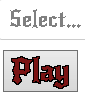
\includegraphics[width=0.1\linewidth]{Imagenes/Fitness4.png}
  \caption{Módulo fitness, imagen de muestra sobre botones de la gamificación para la corrección de mala postura en la espalda. Elaboración propia}
  \label{fig:imagen5fitness}
\end{figure}

\begin{figure}[H]
  \centering
  
\includegraphics[width=0.2\linewidth]{Imagenes/Fitness5.png}
  \caption{Módulo fitness, imagen de muestra sobre elemento puntuación sobre gamificación para la corrección de mala postura en la espalda. Elaboración propia}
  \label{fig:imagen6fitness}
\end{figure}

Finalmente, se añadió una imagen inicial con instrucciones para que el jugador comprendiera tanto los botones como las posiciones que deberá usar durante el juego:
\begin{figure}[H]
  \centering
  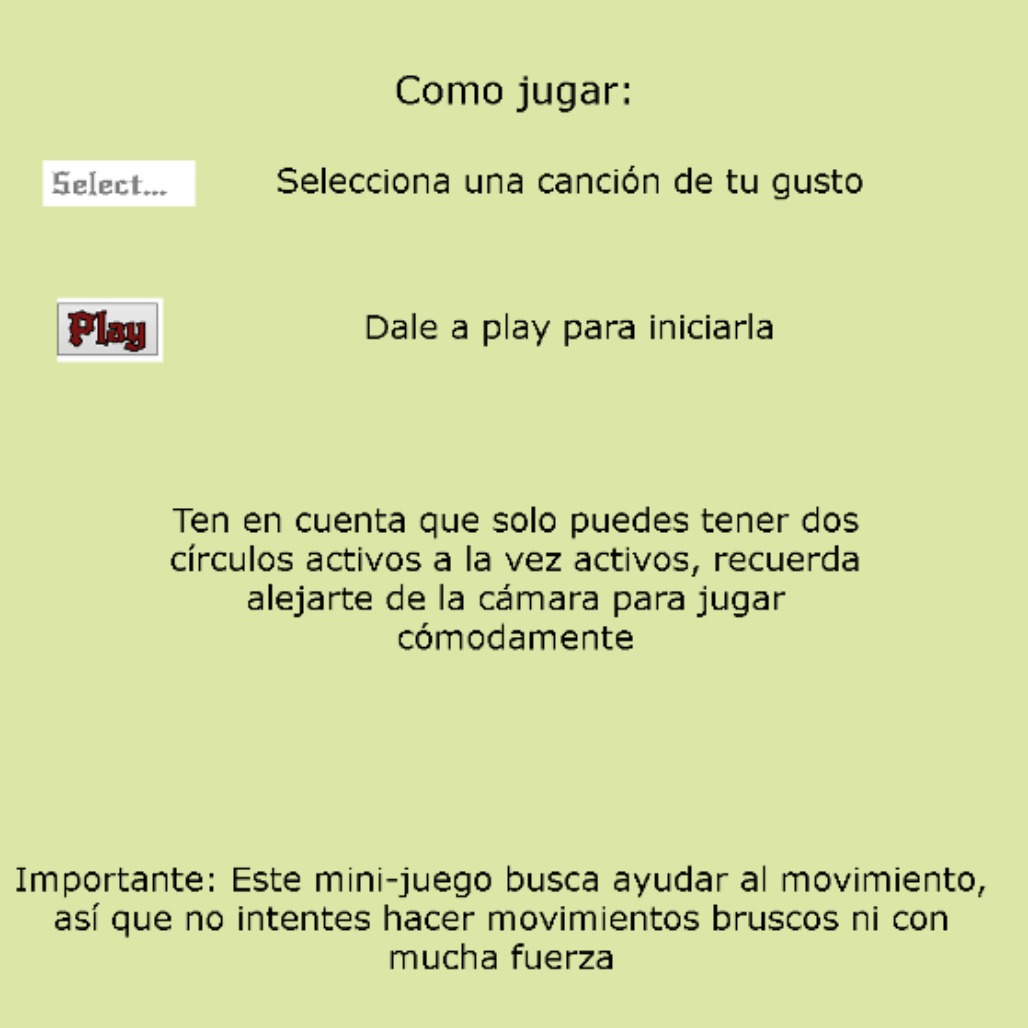
\includegraphics[width=0.5\linewidth]{Imagenes/tuto-espalda.png}
  \caption{Módulo fitness, imagen de tutorial sobre gamificación para la corrección de mala postura en la espalda. Elaboración propia}
  \label{fig:imagen7fitness}
\end{figure}

\subsection{Modulo mindset}
En el desarrollo del módulo de mindset, se decidió agrupar las subhabilidades seleccionadas en el capítulo anterior y utilizar el motor de videojuegos Godot, conocido por su capacidad para crear entornos 2D y 3D multiplataforma, libre y de código abierto. Para este caso de estudio, se optó por usar principalmente su funcionalidad en 2D, desarrollando una serie de niveles enfocados en fomentar habilidades como la capacidad analítica, la interpretación de patrones y la creatividad, entre otras previamente mencionadas. Estos niveles abarcan desde el uso de una balanza para decidir la posición de bloques hasta la interpretación de patrones para elegir el siguiente camino a seguir. A continuación, se presentan los diferentes niveles junto con un breve resumen de cada uno.
\subsubsection{Nivel 1}
El primer nivel se basa en una agrupación de flechas dentro de un laberinto sencillo. La idea es enseñar al jugador que puede interactuar con los objetos, fomentando así la exploración y la interacción en el entorno de juego.

\begin{figure}[H]
  \centering
  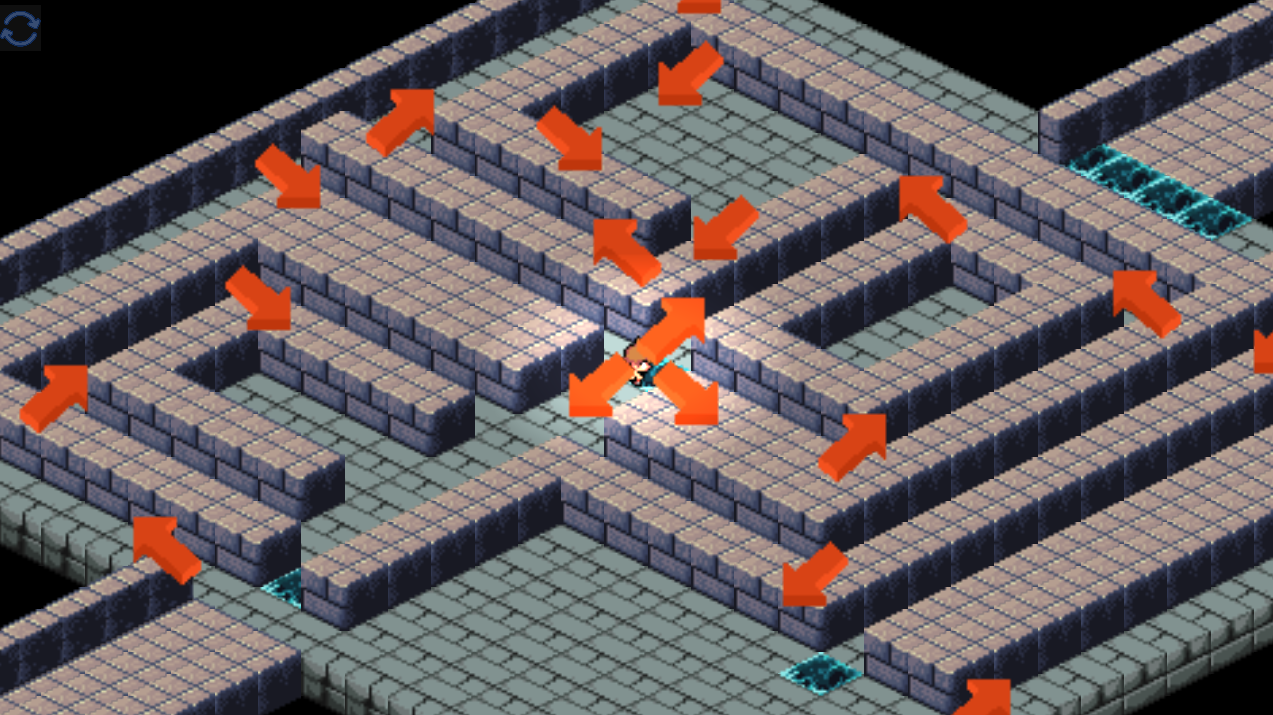
\includegraphics[width=0.7\linewidth]{Imagenes/Nivel1.png}
  \caption{Módulo mindset, imagen de referencia sobre gamificación para el módulo mindset, Nivel 1. Elaboración propia}
  \label{fig:imagen1mindset}
\end{figure}


\subsubsection{Nivel 2}

El segundo nivel se basa en una balanza con la cual el jugador debe interactuar para comparar el peso de dos objetos y ordenarlos según su peso. Este nivel busca fomentar el razonamiento lógico del jugador.

\begin{figure}[H]
  \centering
  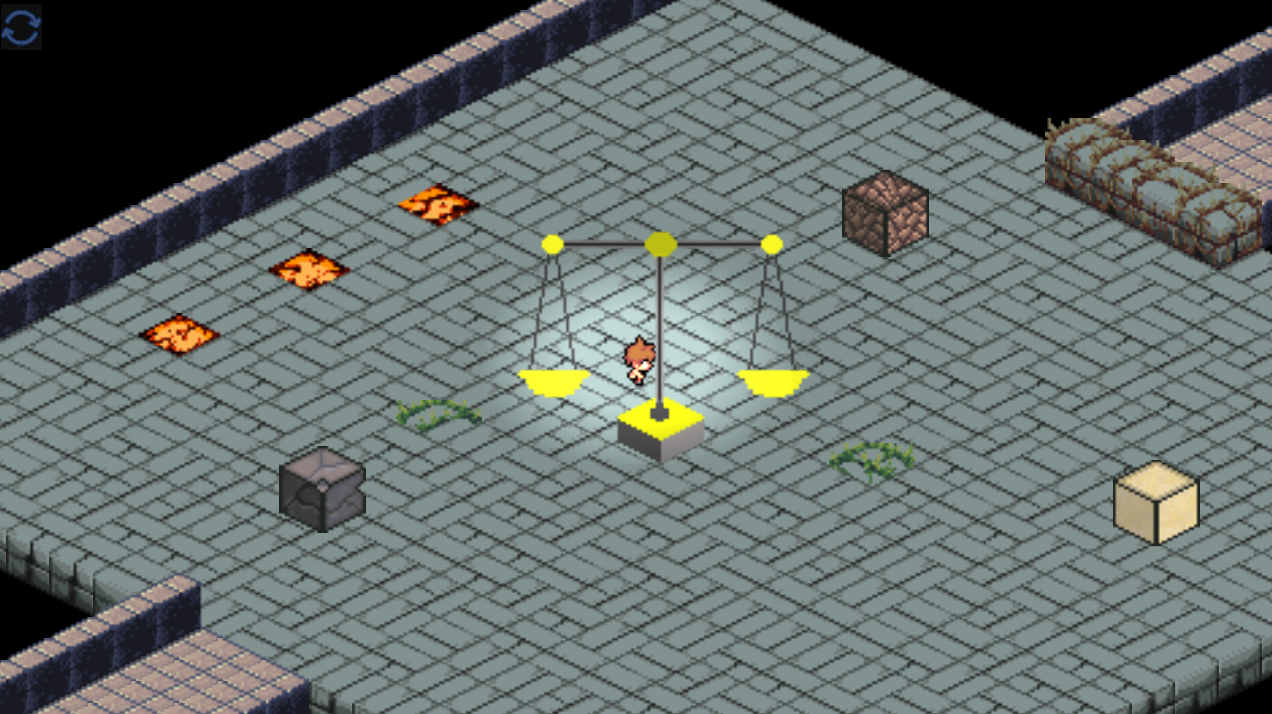
\includegraphics[width=0.7\linewidth]{Imagenes/Nivel2.png}
  \caption{Módulo mindset, imagen de referencia sobre gamificación para el módulo mindset, Nivel 2. Elaboración propia}
  \label{fig:imagen1mindset}
\end{figure}

\subsubsection{Nivel 3}
El tercer nivel se basa en un conjunto de portales: algunos permiten el paso del jugador y otros solo permiten el paso de cajas. El objetivo es llevar dos cajas hasta el final para abrir una puerta. Este nivel busca desarrollar principalmente la paciencia, ya que, al ser de varios portales, si mueves una caja demasiado rápido, podrías colocarla sobre un portal destinado solo para el jugador, lo cual te teletransportaría al tocarlo y te obligaría a reiniciar el nivel al perder acceso a la caja.

\begin{figure}[H]
  \centering
  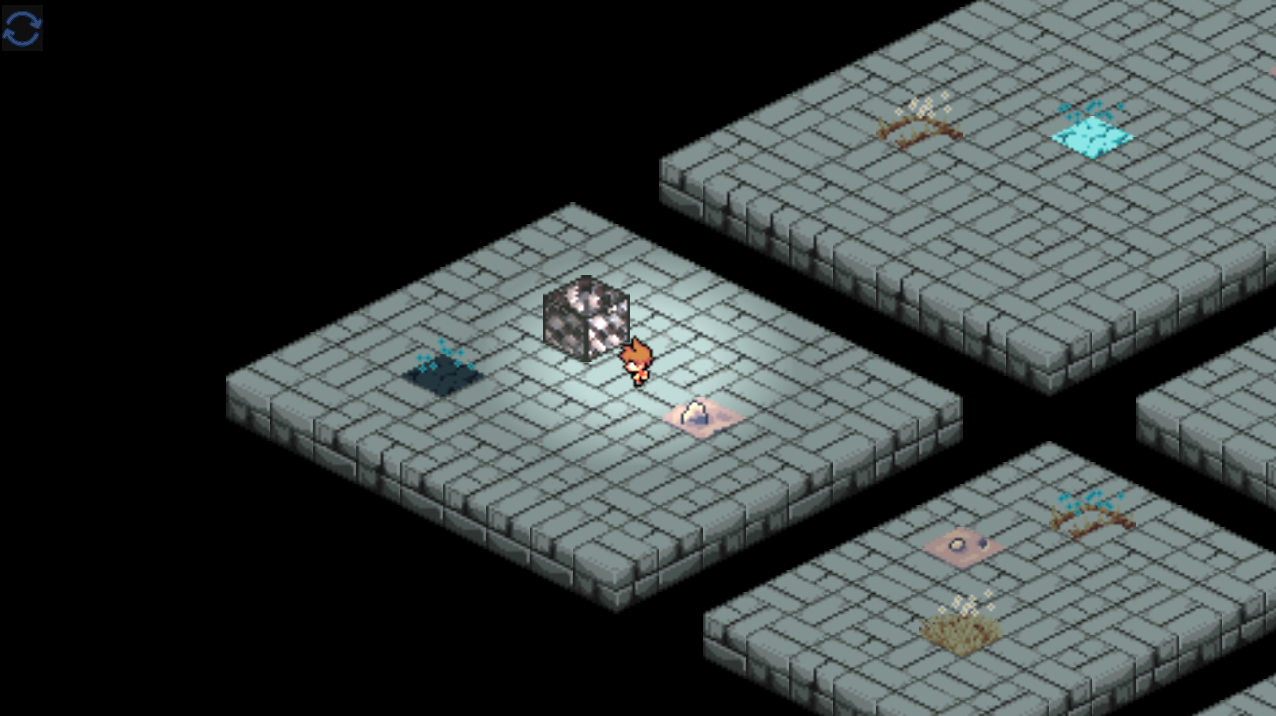
\includegraphics[width=0.7\linewidth]{Imagenes/Nivel3.png}
  \caption{Módulo mindset, imagen de referencia sobre gamificación para el módulo mindset, Nivel 3. Elaboración propia}
  \label{fig:imagen1mindset}
\end{figure}
\subsubsection{Nivel 4}
El cuarto nivel se basa en una serie de portales, donde, a partir de sutiles pistas en el escenario, el jugador puede identificar cuál es el correcto. En total, consiste en varios portales que varían en la forma de diferenciarse. Elegir un portal incorrecto devolverá al inicio del nivel, y el objetivo es fomentar la habilidad de deducción en el jugador.

\begin{figure}[H]
  \centering
  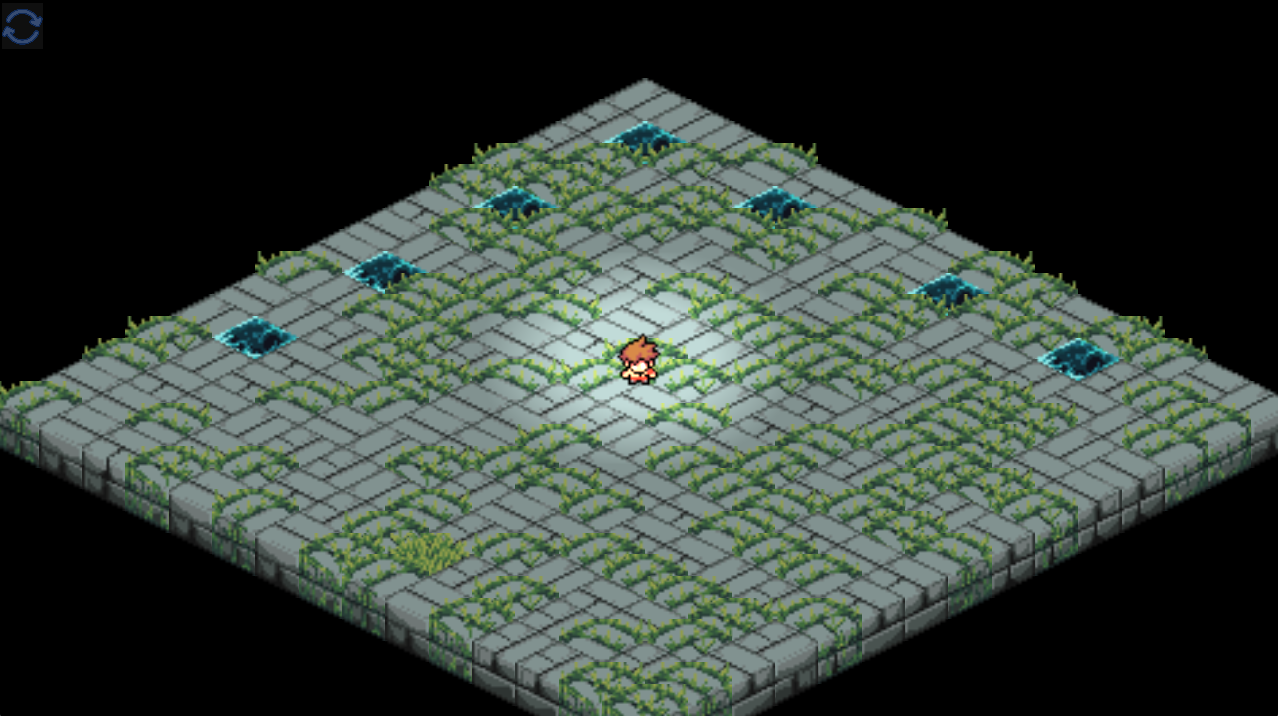
\includegraphics[width=0.7\linewidth]{Imagenes/Nivel4.png}
  \caption{Módulo mindset, imagen de referencia sobre gamificación para el módulo mindset, Nivel 4. Elaboración propia}
  \label{fig:imagen1mindset}
\end{figure}

\subsubsection{Nivel 5}
El quinto y último nivel se basa en un laberinto con visibilidad limitada, el cual tiene una sutil marca que muestra el camino correcto. Si el jugador toma un camino diferente, será devuelto al inicio del laberinto. Debido a la baja visibilidad, el jugador podría no darse cuenta de que está regresando al punto de partida, lo que puede llevarlo a dar vueltas sin saberlo. Este nivel busca fomentar tanto la capacidad de deducción como, principalmente, la paciencia del jugador, al motivarlo a probar diferentes métodos para completar el desafío.

\begin{figure}[H]
  \centering
  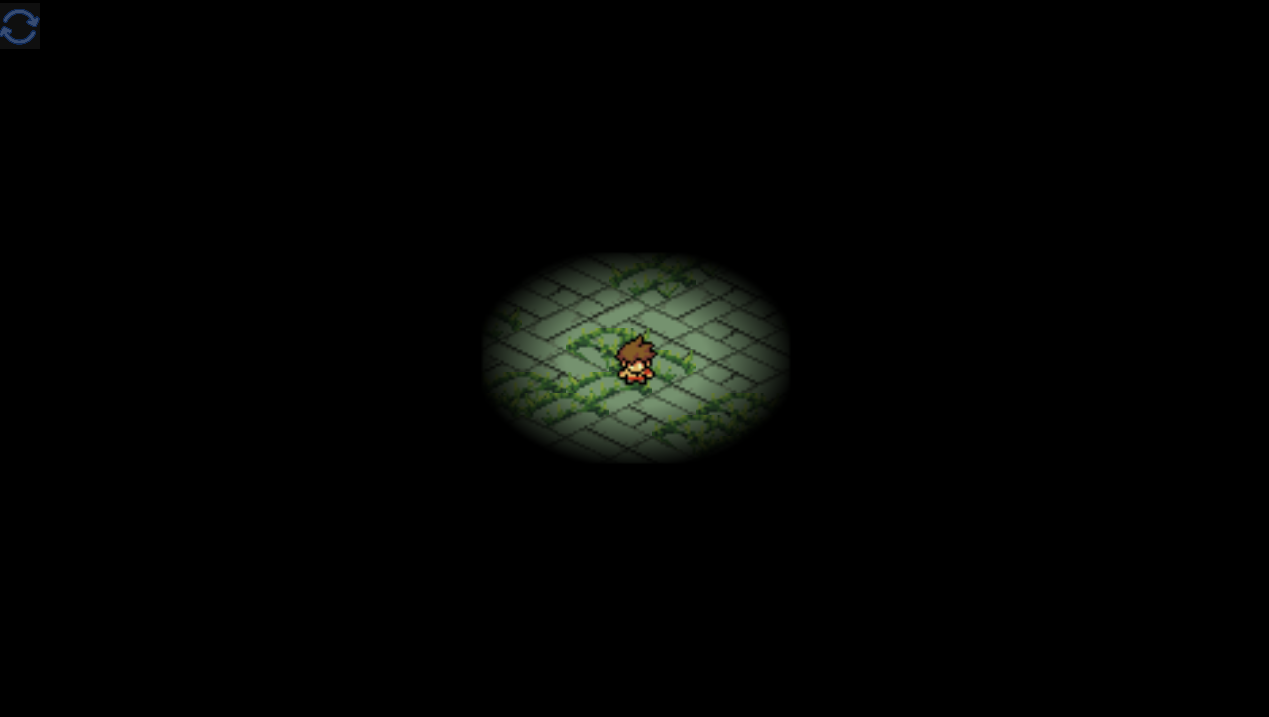
\includegraphics[width=0.7\linewidth]{Imagenes/Nivel5.png}
  \caption{Módulo mindset, imagen de referencia sobre gamificación para el módulo mindset, Nivel 5. Elaboración propia}
  \label{fig:imagen1mindset}
\end{figure}

%pruebas

\chapter{Pruebas de los modulos}
\section{Experimentacìon y pruebas}
En este capítulo se llevan a cabo pruebas a los módulos desarrollados con el objetivo de realizar un estudio que permita identificar áreas de mejora y optimizar su funcionamiento futuro.
\subsection{Pruebas funcionales}
Mediante el uso de Selenium, una herramienta automatizada para realizar pruebas funcionales en aplicaciones web, se evaluaron las diferentes partes de los módulos, tanto de forma individual como conjunta. Esto permitió verificar su correcto funcionamiento y detectar posibles errores o áreas de mejora en la interacción del usuario con cada módulo.
En cada uno de los casos, se verificó el funcionamiento de todos los botones disponibles, tanto los botones físicos como aquellos ubicados en la interfaz. Se realizaron pruebas exhaustivas para asegurar que cada botón respondiera correctamente y ejecutará las acciones esperadas, garantizando una interacción fluida y sin errores en el uso de los módulos.A continuación, se presentan los resultados e instrucciones obtenidas en las pruebas conjuntas. Para la revisión de las pruebas individuales, ir a la sección de anexos.

\subsubsection{Pruebas conjuntas}

\begin{figure}[ht]
  \centering
  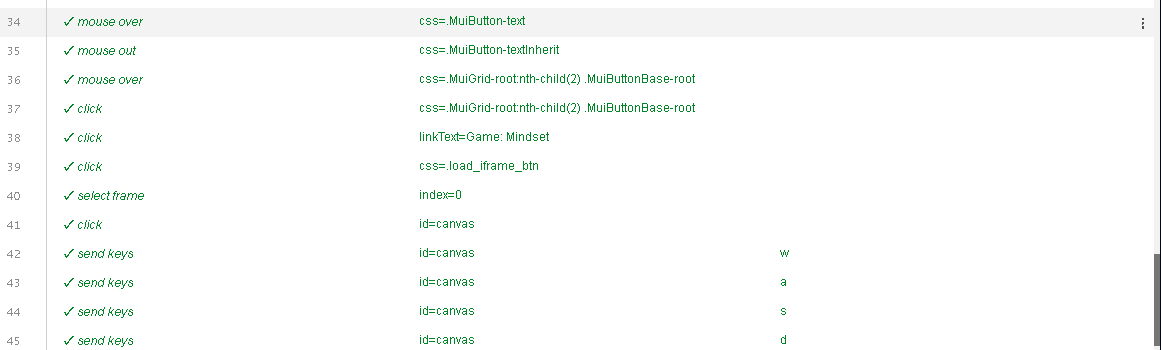
\includegraphics[width=1\linewidth]{Imagenes/Imagen11.png}
  \caption{Imagen de referencia sobre instrucciones de gamificación para los módulos conjuntos,Elaboración propia}
  \label{fig:imagen1pruebas}
\end{figure}
\begin{figure}[ht]
  \centering
  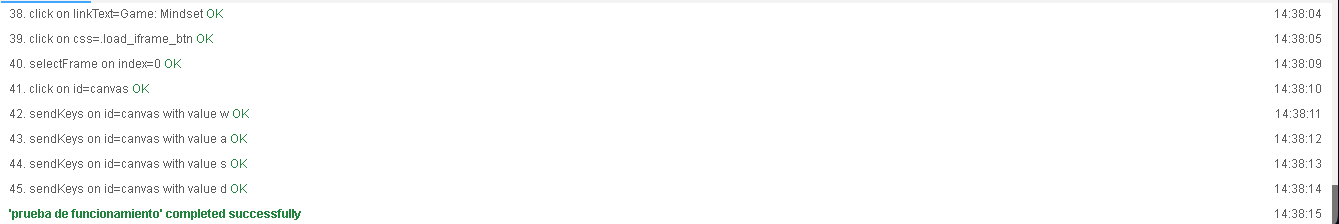
\includegraphics[width=1\linewidth]{Imagenes/Imagen12.png}
  \caption{Imagen de referencia sobre resultados de gamificación para los módulos conjuntos,Elaboración propia}
  \label{fig:imagen2pruebas}
\end{figure}

\subsection{Pruebas de usabilidad en voz alta}

Se realizaron tres pruebas de usabilidad en voz alta, las cuales consisten en pedir a los usuarios que verbalicen sus pensamientos mientras interactúan con un software. A continuación, se presenta un breve resumen de lo observado en cada una.

\subsubsection{Prueba 1}
La primera prueba tuvo una duración de 36 minutos. Esta comenzó con el módulo fitness, específicamente con la sección para la corrección de la mala postura, la cual transcurrió con normalidad. El usuario se mostró animado durante esta etapa.
Se continuó con la segunda sección del mismo módulo, que también transcurrió sin dificultades. El usuario mantuvo una actitud tranquila a lo largo de esta parte.
\\\\
Posteriormente, se pasó al módulo mindset, donde se realizaron los dos primeros niveles sin inconvenientes. El usuario se mostró animado durante estas actividades.
\\\\
Al llegar al tercer nivel, presentó algunas dificultades con el movimiento del personaje. Sin embargo, continuó al cuarto nivel, donde, tras un breve periodo de observación, completó el nivel rápidamente. Finalmente, en el último nivel, el usuario solicitó asistencia para completarlo, lo que evidencia un grado de dificultad probablemente demasiado elevado.

\subsubsection{Prueba 2}

La segunda prueba tuvo una duración de 1 hora y 38 minutos. Comenzó con la gamificación sobre el mindset,
 la cual no presentó mayores impedimentos para completar el nivel 1 de manera rápida.
  Sin embargo, el segundo nivel requirió un tiempo considerable, aproximadamente 35 minutos, 
  donde se observó un entendimiento de la utilidad de la balanza, aunque surgieron problemas 
  para identificar el orden correcto en el que se debían colocar los bloques.
\\\\
El tercer nivel se completó de forma normal y no presentó grandes dificultades.
 En el cuarto nivel, aunque inicialmente hubo un poco de dificultad para comprender las mecánicas,
  se logró superar de forma rápida tras entenderlas. Finalmente, el último nivel tomó alrededor
   de 25 minutos en completarse. Durante este nivel, el usuario presentó dificultades significativas
    y tuvo que solicitar asistencia, lo que indica que la dificultad podría ser demasiado elevada.
  \\  \\
    Posteriormente, se continuó con la sección para la corrección de la mala postura en el módulo fitness, la cual no presentó dificultad alguna y prosiguió con normalidad. Sin embargo, es importante destacar que, después de un tiempo, el usuario parecía aburrirse debido a la baja velocidad del desarrollo una vez que se acostumbró a la dinámica del ejercicio.
\\\\
Finalmente, se pasó a la sección destinada a los ejercicios para ayudar con el túnel carpiano en el módulo fitness. En esta parte, no se presentaron mayores dificultades, salvo por los primeros momentos, donde el usuario tuvo problemas para comprender los controles del ejercicio.

\subsubsection{Prueba 3}
La tercera prueba tuvo una duración de 34 minutos.
La prueba comenzó con la sección de corrección de la postura del módulo fitness, la cual se completó sin ninguna dificultad. El usuario se mostró animado durante esta parte.
\\\\
Posteriormente, inició la segunda sección del mismo módulo, enfocada en ejercicios para ayudar con el túnel carpiano. Aunque presentó una leve dificultad para comprender las instrucciones al inicio, pudo continuar sin complicaciones tras unos momentos.
\\\\
A continuación, el usuario pasó al módulo mindset. Completó el primer nivel sin dificultades y logró superar el segundo nivel por mera casualidad, sin necesidad de utilizar la balanza.
En el tercer nivel, comprendió rápidamente la mecánica, y aunque necesitó varios intentos, logró completarlo con éxito. El cuarto nivel lo superó a base de repetición e intentos, hasta que comprendió las pistas necesarias para avanzar.
\\\\
Finalmente, en el último nivel, el usuario lo completó basándose en su memoria y repeticiones previas, sin necesitar de las pistas proporcionadas en el juego.


%Resultados
\chapter{Resultados}

Se realizaron dos encuestas sobre la aplicación. La primera fue aplicada a más de 50 estudiantes de la carrera de Ingeniería en Sistemas de la Universidad del Valle, quienes respondieron después de probar la aplicación. La segunda encuesta se dirigió a expertos y personas con experiencia en el campo de sistemas, utilizando una evaluación basada en las heurísticas de Nielsen. A continuación, se presentan los resultados junto con un breve análisis de los mismos.
\section{Cuestionario sobre evaluación de experiencia en softskills para los módulos Mindset y Fitness}
\subsection{Fitness: Juego sobre movimiento de la muñeca}
La pregunta ``El juego es fácil de entender y aprender`` obtuvo la mayor cantidad de respuestas en la opción 4, con 29 votos. Esto indica que el juego es relativamente sencillo de comprender, pero aún tiene margen de mejora. La observación más común fue que la posición en ángulo recto de la palma puede resultar un poco confusa.

    \begin{figure}[H]
  \centering
  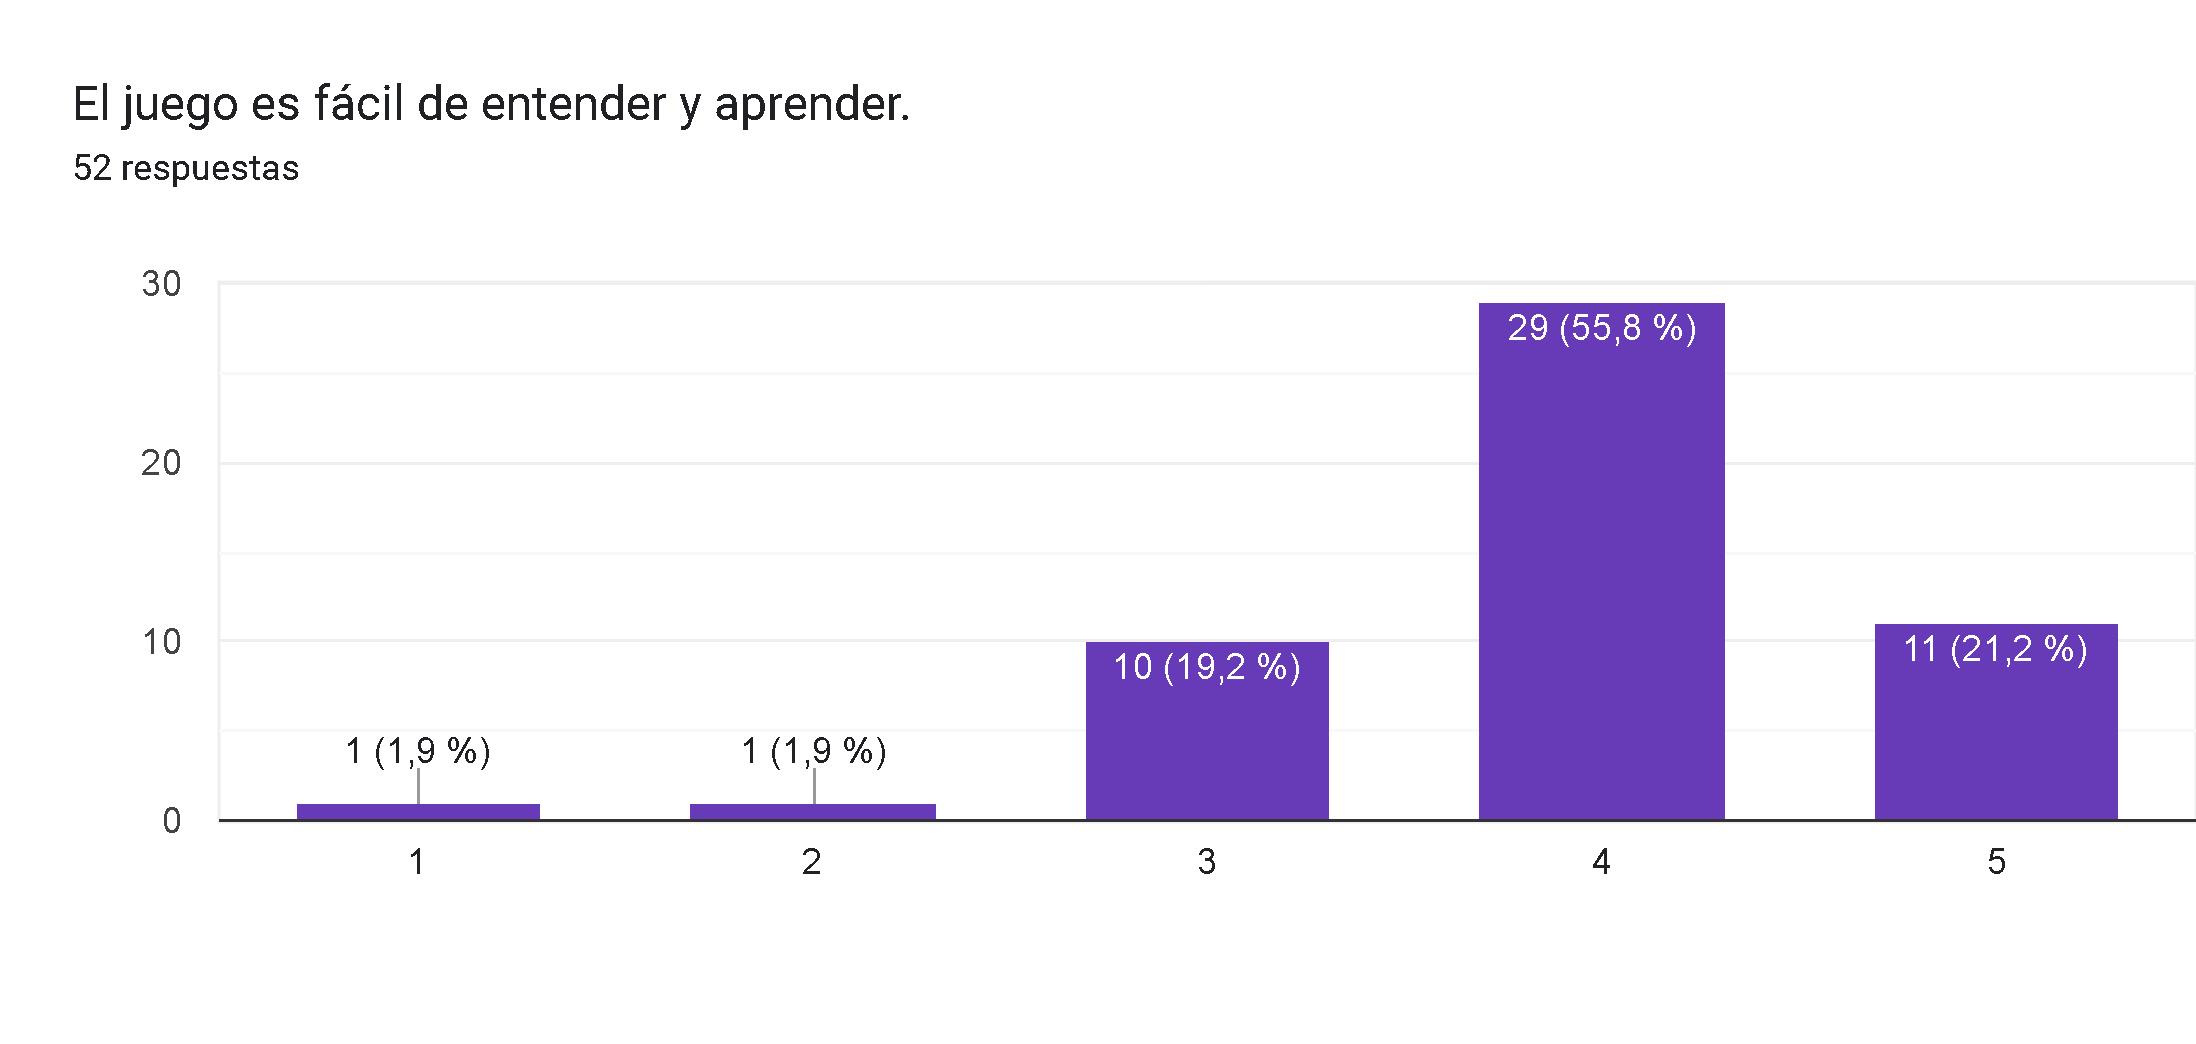
\includegraphics[width=0.7\linewidth]{Imagenes/fc1.png}
  \caption{Elaboración propia, Módulo fitness, Imagen de referencia sobre cuestionario  de gamificación para el módulo fitness del juego sobre la muñeca, ``El juego es fácil de entender y aprender``}
  \label{fig:cuestionario1fitness}
\end{figure}



La pregunta ``Los controles son intuitivos y responden bien`` obtuvo la mayor cantidad de respuestas en la opción 4, con un 40,4 \%. Esto sugiere que los controles son mayormente funcionales e intuitivos, aunque aún hay oportunidad de optimización para una experiencia más fluida.

    \begin{figure}[H]
  \centering
  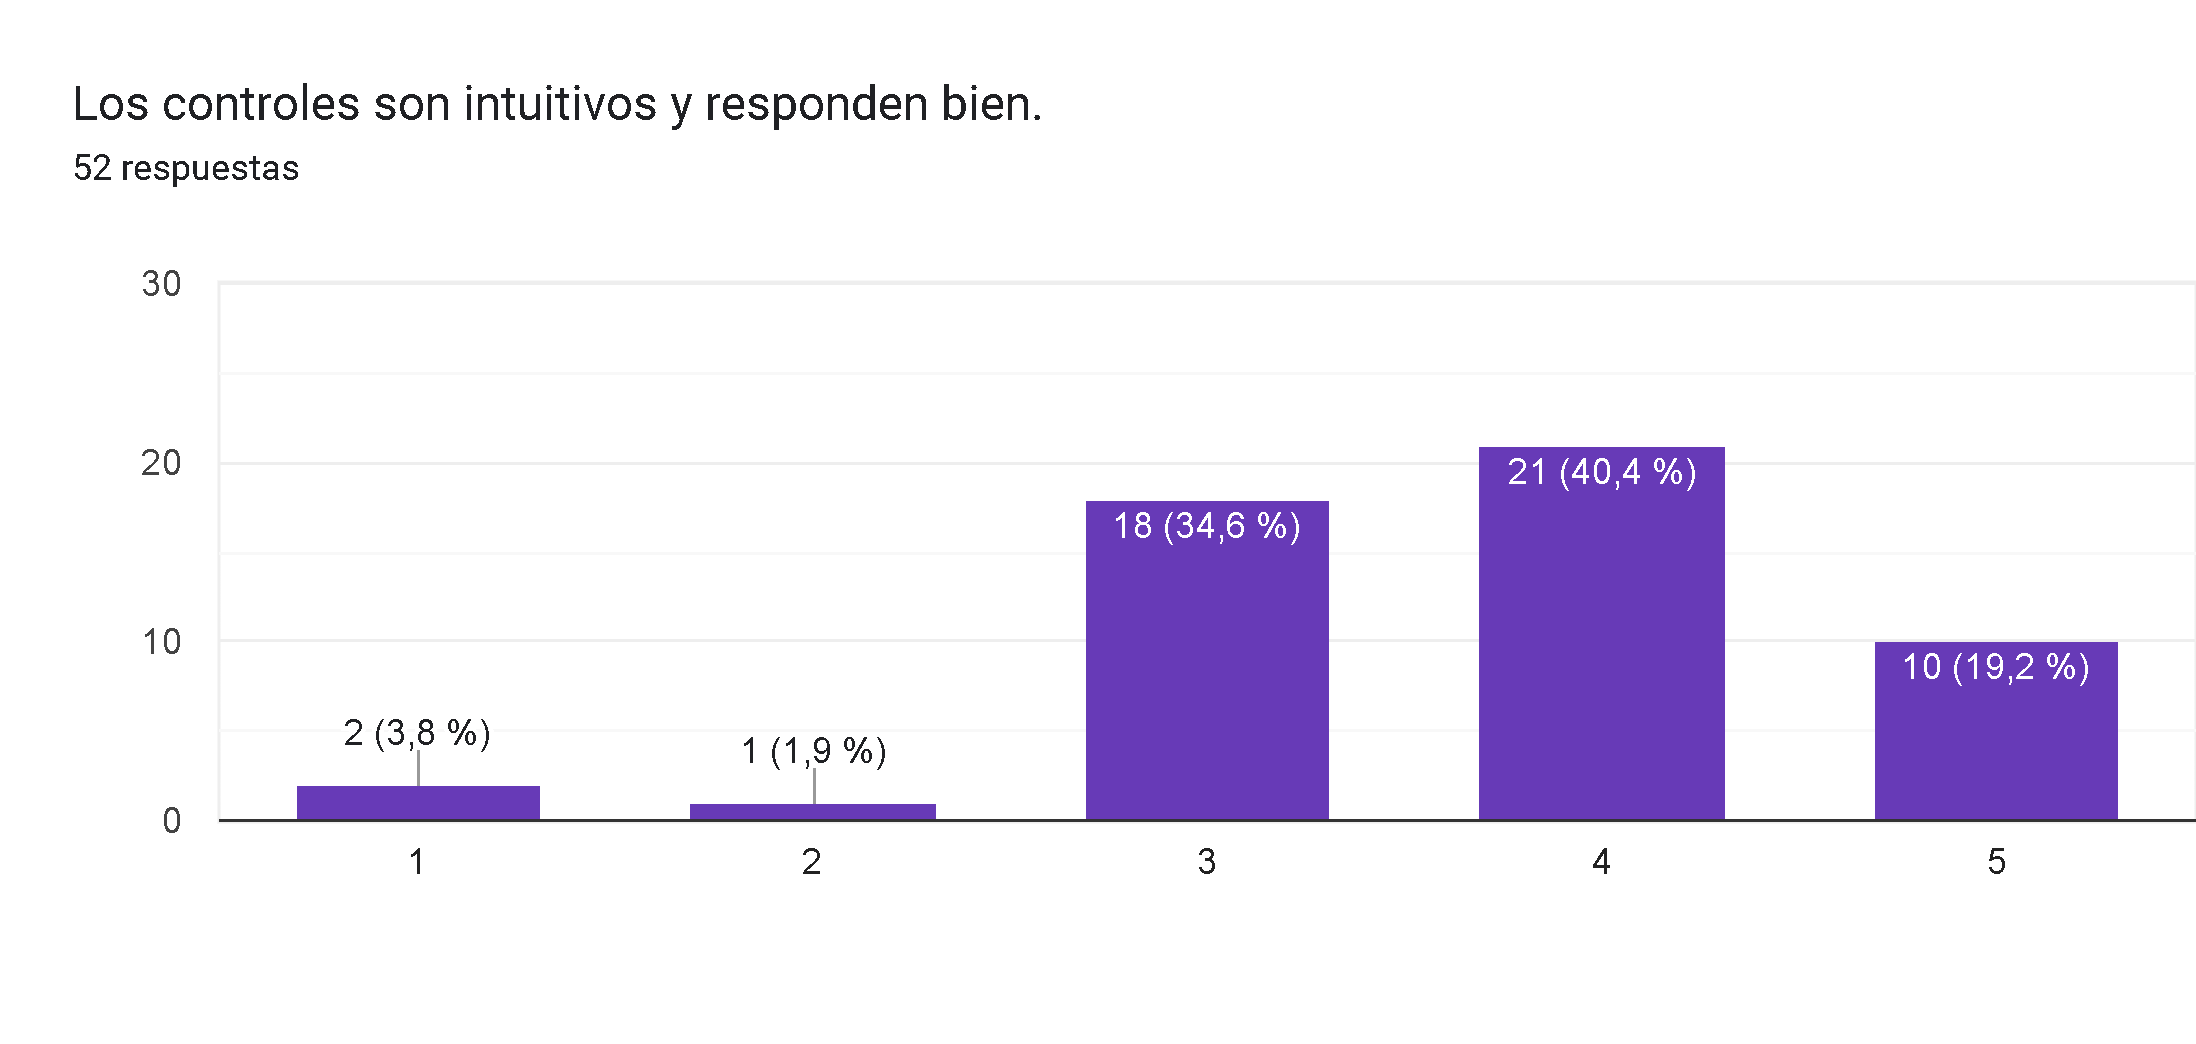
\includegraphics[width=0.7\linewidth]{Imagenes/fc2.png}
  \caption{Elaboración propia, Módulo fitness, Imagen de referencia sobre cuestionario  de gamificación para el módulo fitness del juego sobre la muñeca,  ``Los controles son intuitivos y responden bien``}
  \label{fig:cuestionario2fitness}
\end{figure}
La pregunta ``El nivel de dificultad es adecuado`` obtuvo la mayor cantidad de respuestas en la opción 4, con un 57,7 \%. Esto sugiere que la mayoría de los usuarios considera que la dificultad está bien equilibrada, aunque una parte significativa podría encontrarla demasiado fácil o desafiante.

 \begin{figure}[H]
  \centering
  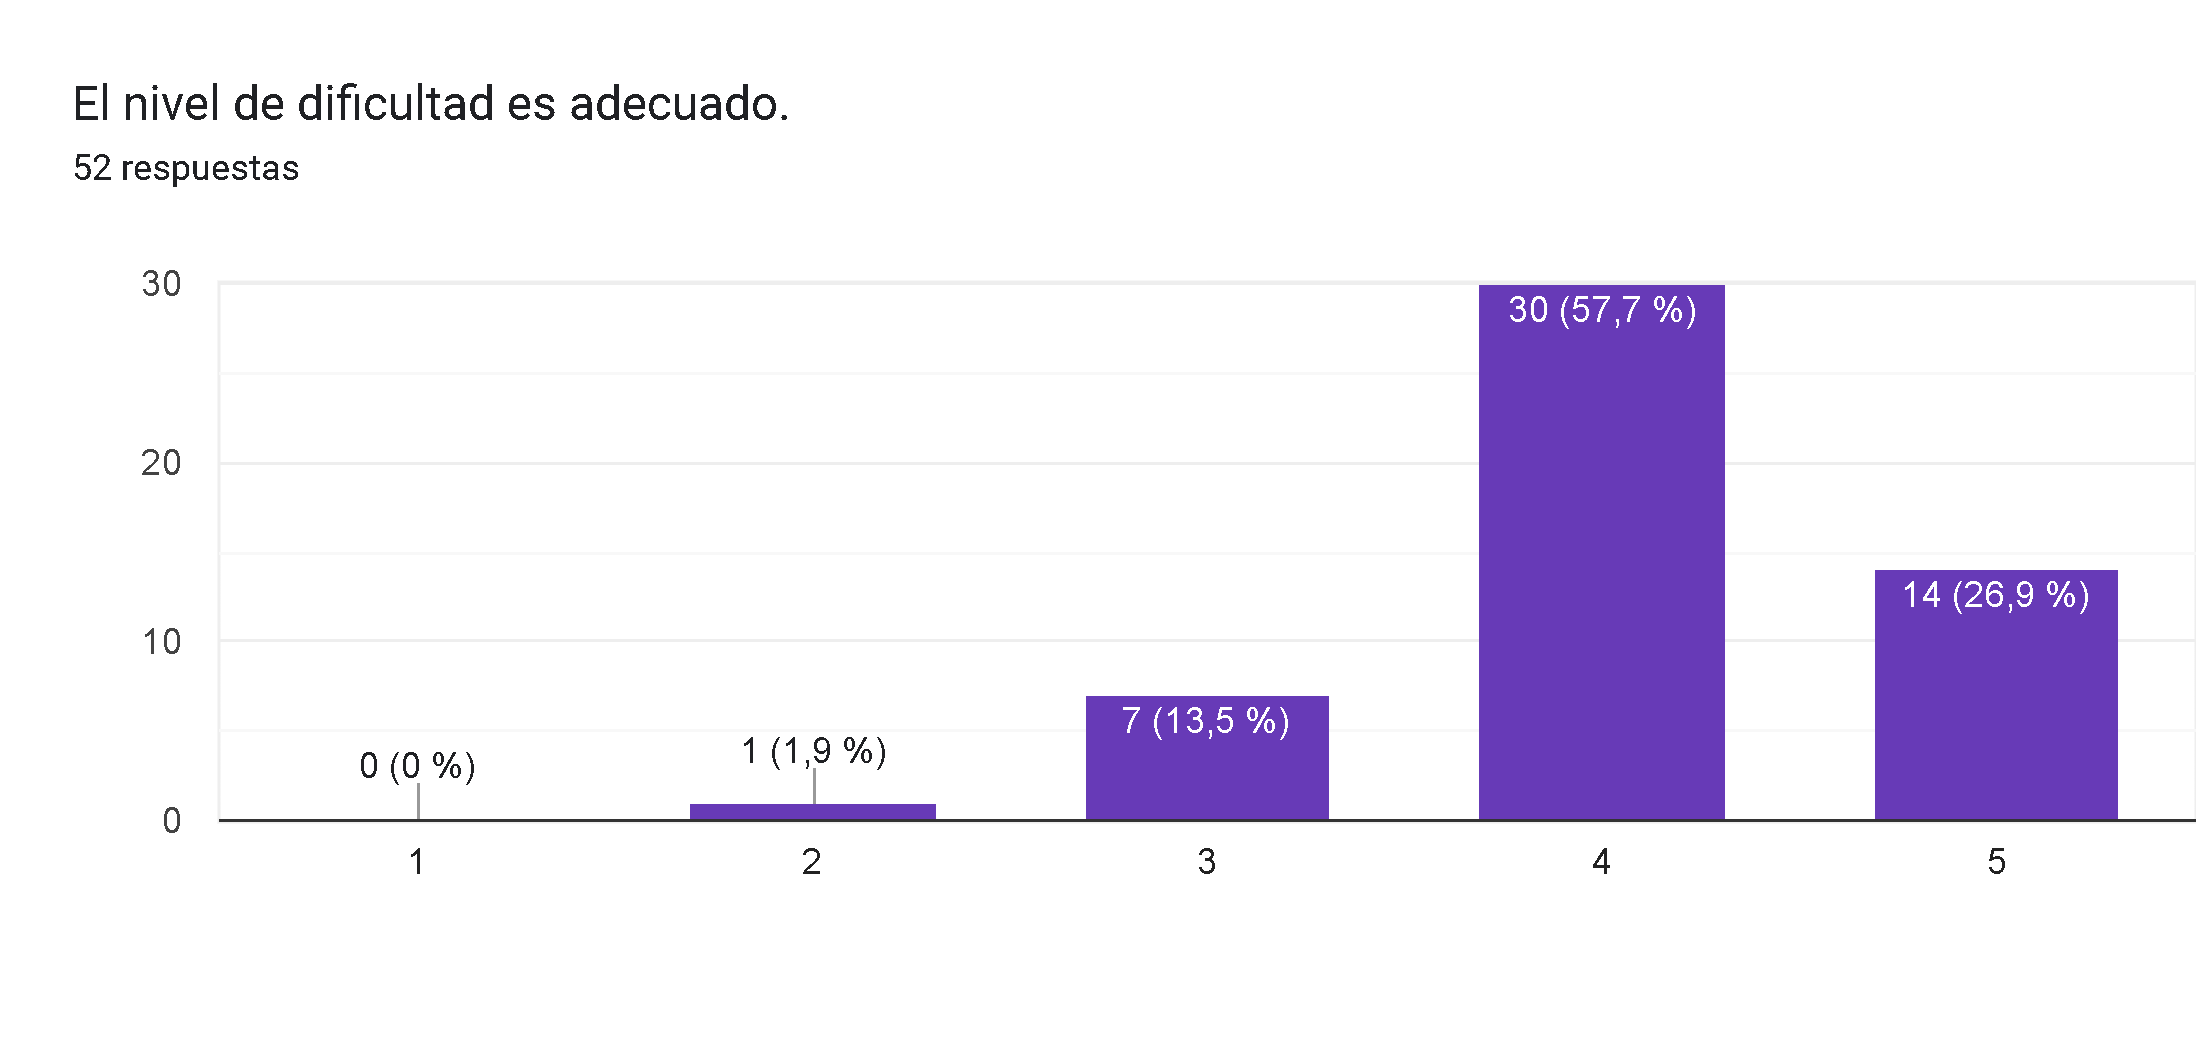
\includegraphics[width=0.7\linewidth]{Imagenes/fc3.png}
  \caption{Elaboración propia, Módulo fitness, Imagen de referencia sobre cuestionario  de gamificación para el módulo fitness del juego sobre la muñeca,  ``El nivel de dificultad es adecuado``}
  \label{fig:cuestionario3fitness}
\end{figure}

La pregunta ``El juego detecta mis movimientos corporales de manera precisa`` obtuvo 20 votos en la opción 3 y 20 en la opción 4, reflejando un puntaje medio. Una observación recurrente fue que la cámara no detecta correctamente la mano si esta lleva un guante de un color similar al fondo. No obstante, dado que no obtuvo una calificación baja, se considera satisfactorio, aunque con posibilidades de mejora.


    \begin{figure}[H]
  \centering
  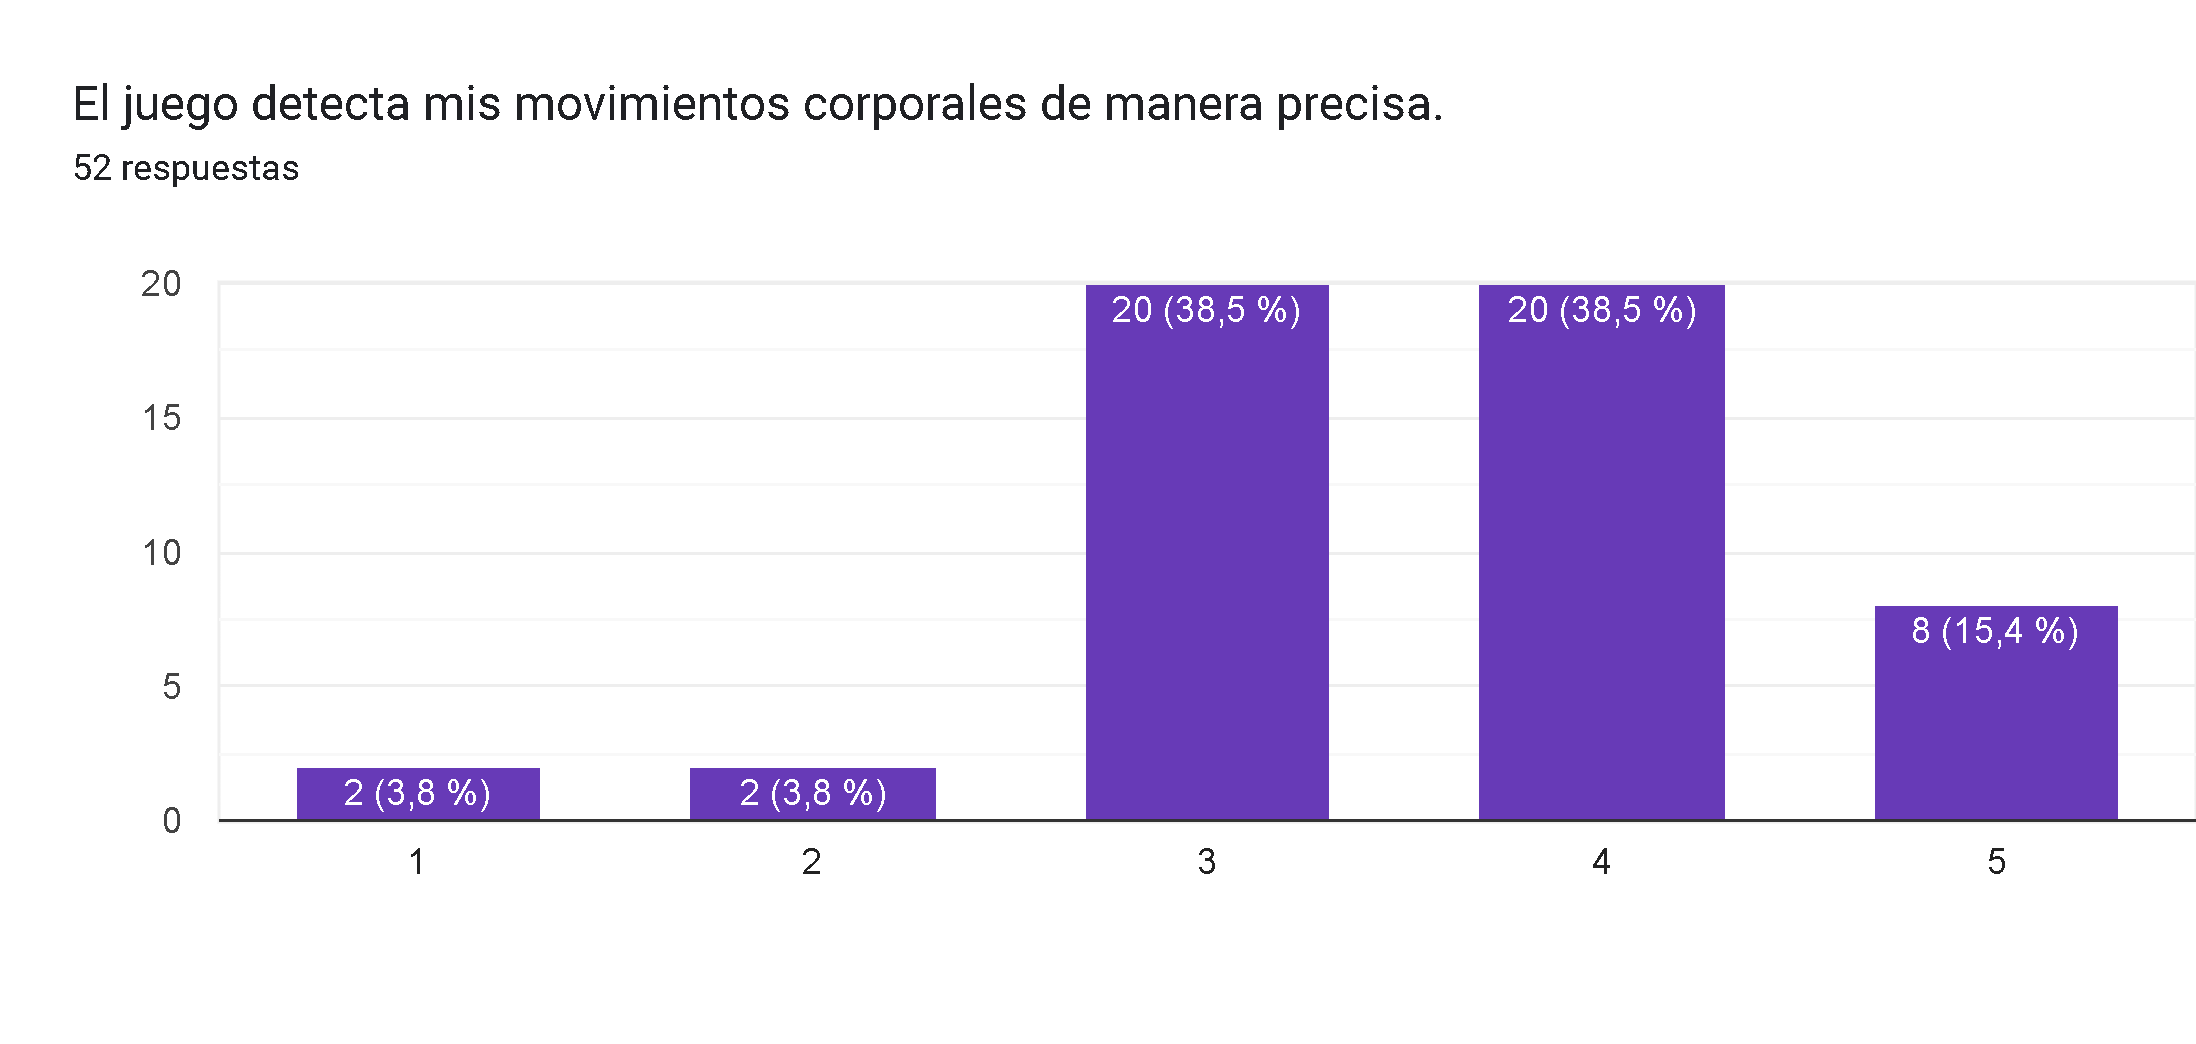
\includegraphics[width=0.7\linewidth]{Imagenes/fc4.png}
  \caption{Elaboración propia, Módulo fitness, Imagen de referencia sobre cuestionario  de gamificación para el módulo fitness del juego sobre la muñeca, ``El juego detecta mis movimientos corporales de manera precisa``}
  \label{fig:cuestionario4fitness}
\end{figure}

La pregunta ``Los movimientos requeridos no provocan fatiga o molestias físicas`` tuvo una respuesta muy positiva, con 24 votos en la opción 5 y ninguno en la opción 1. Esto indica que los movimientos no generaron problemas físicos en la audiencia, siendo bien recibidos por los participantes.

    \begin{figure}[H]
  \centering
  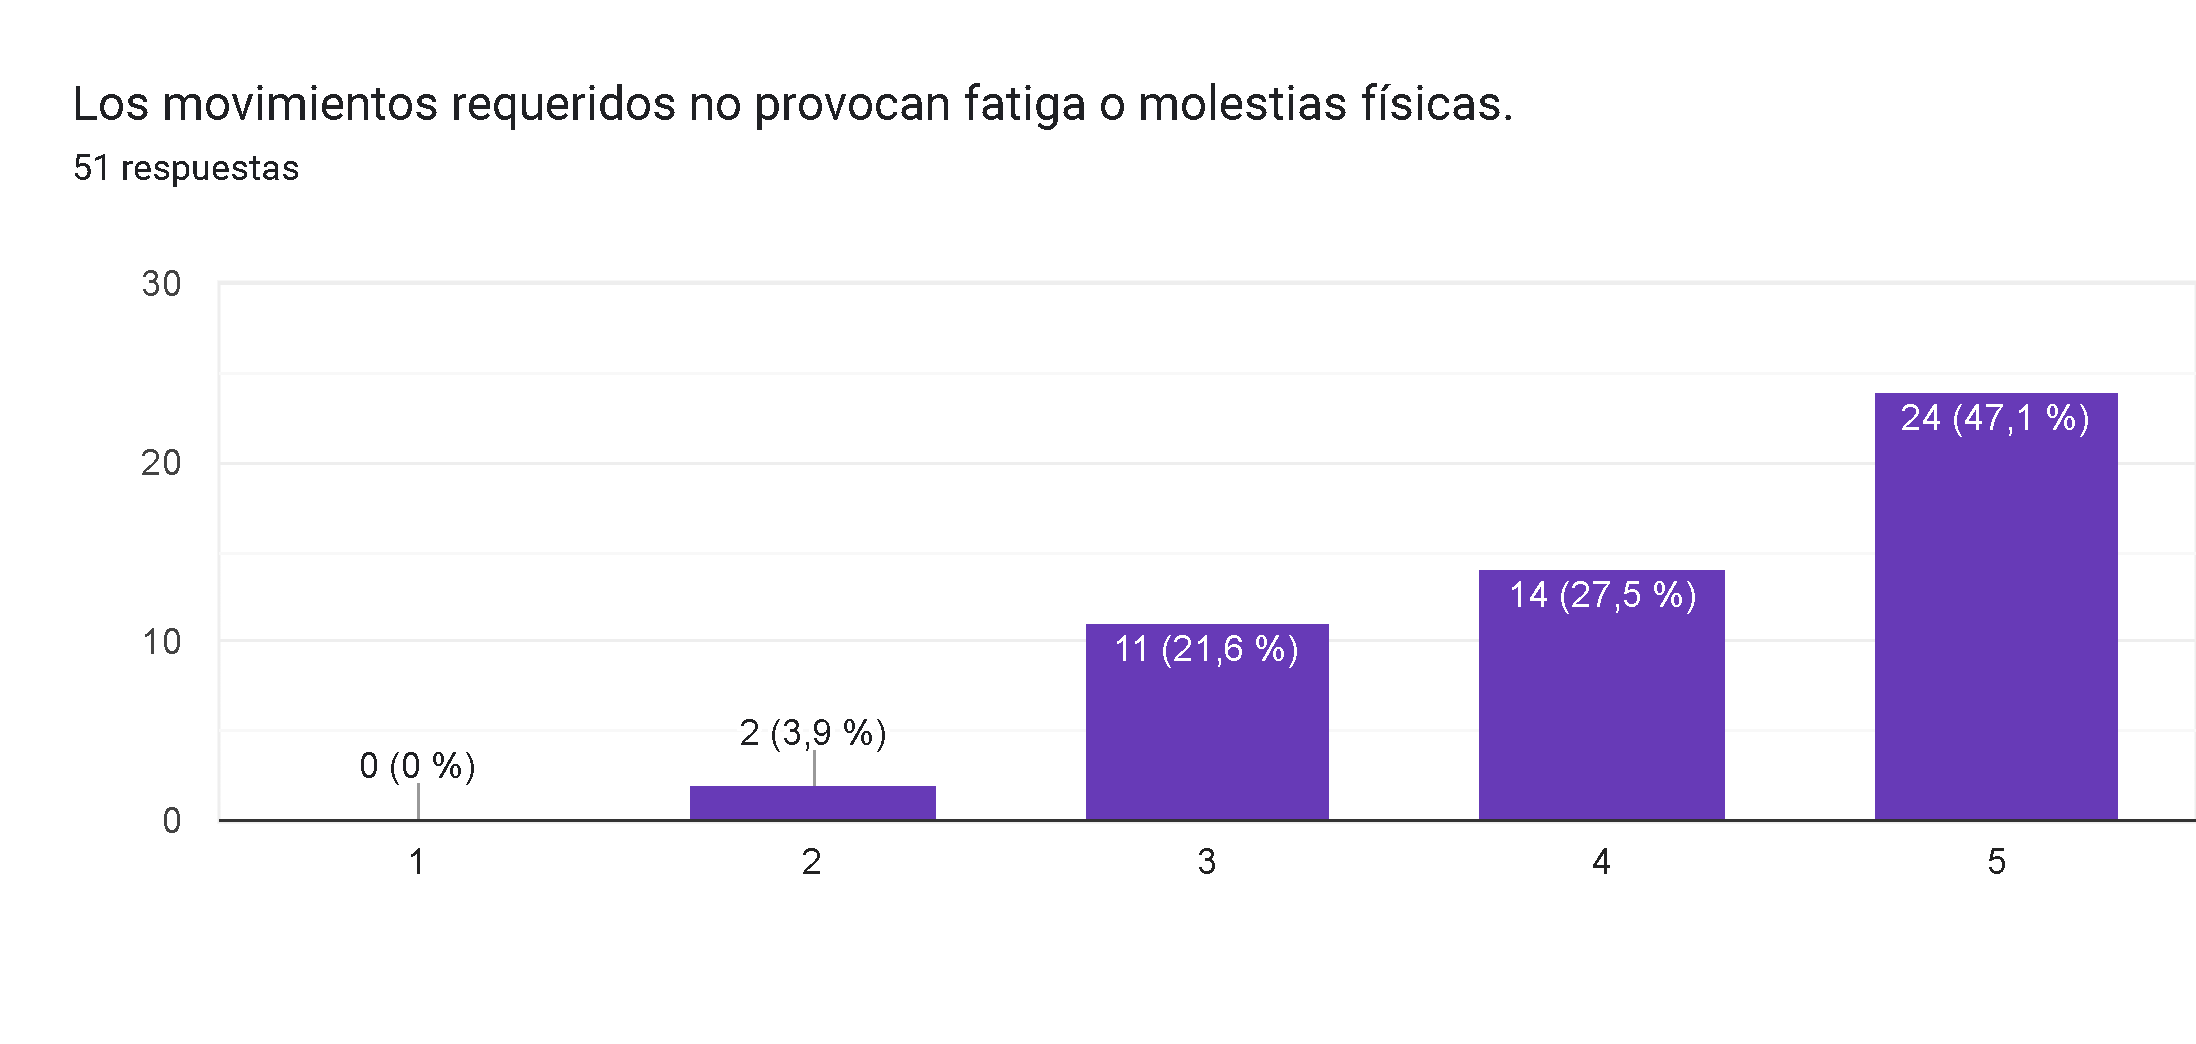
\includegraphics[width=0.7\linewidth]{Imagenes/fc5.png}
  \caption{Elaboración propia, Módulo fitness, Imagen de referencia sobre cuestionario  de gamificación para el módulo fitness del juego sobre la muñeca, ``Los movimientos requeridos no provocan fatiga o molestias físicas``}
  \label{fig:cuestionario5fitness}
\end{figure}


La pregunta ``La interfaz del usuario es clara y fácil de usar`` obtuvo la mayor cantidad de respuestas en la opción 4, con un 30,8 \%. Esto indica que la interfaz es generalmente considerada clara y fácil de usar, aunque algunos usuarios podrían sugerir mejoras para una mayor simplicidad o accesibilidad.

    \begin{figure}[H]
  \centering
  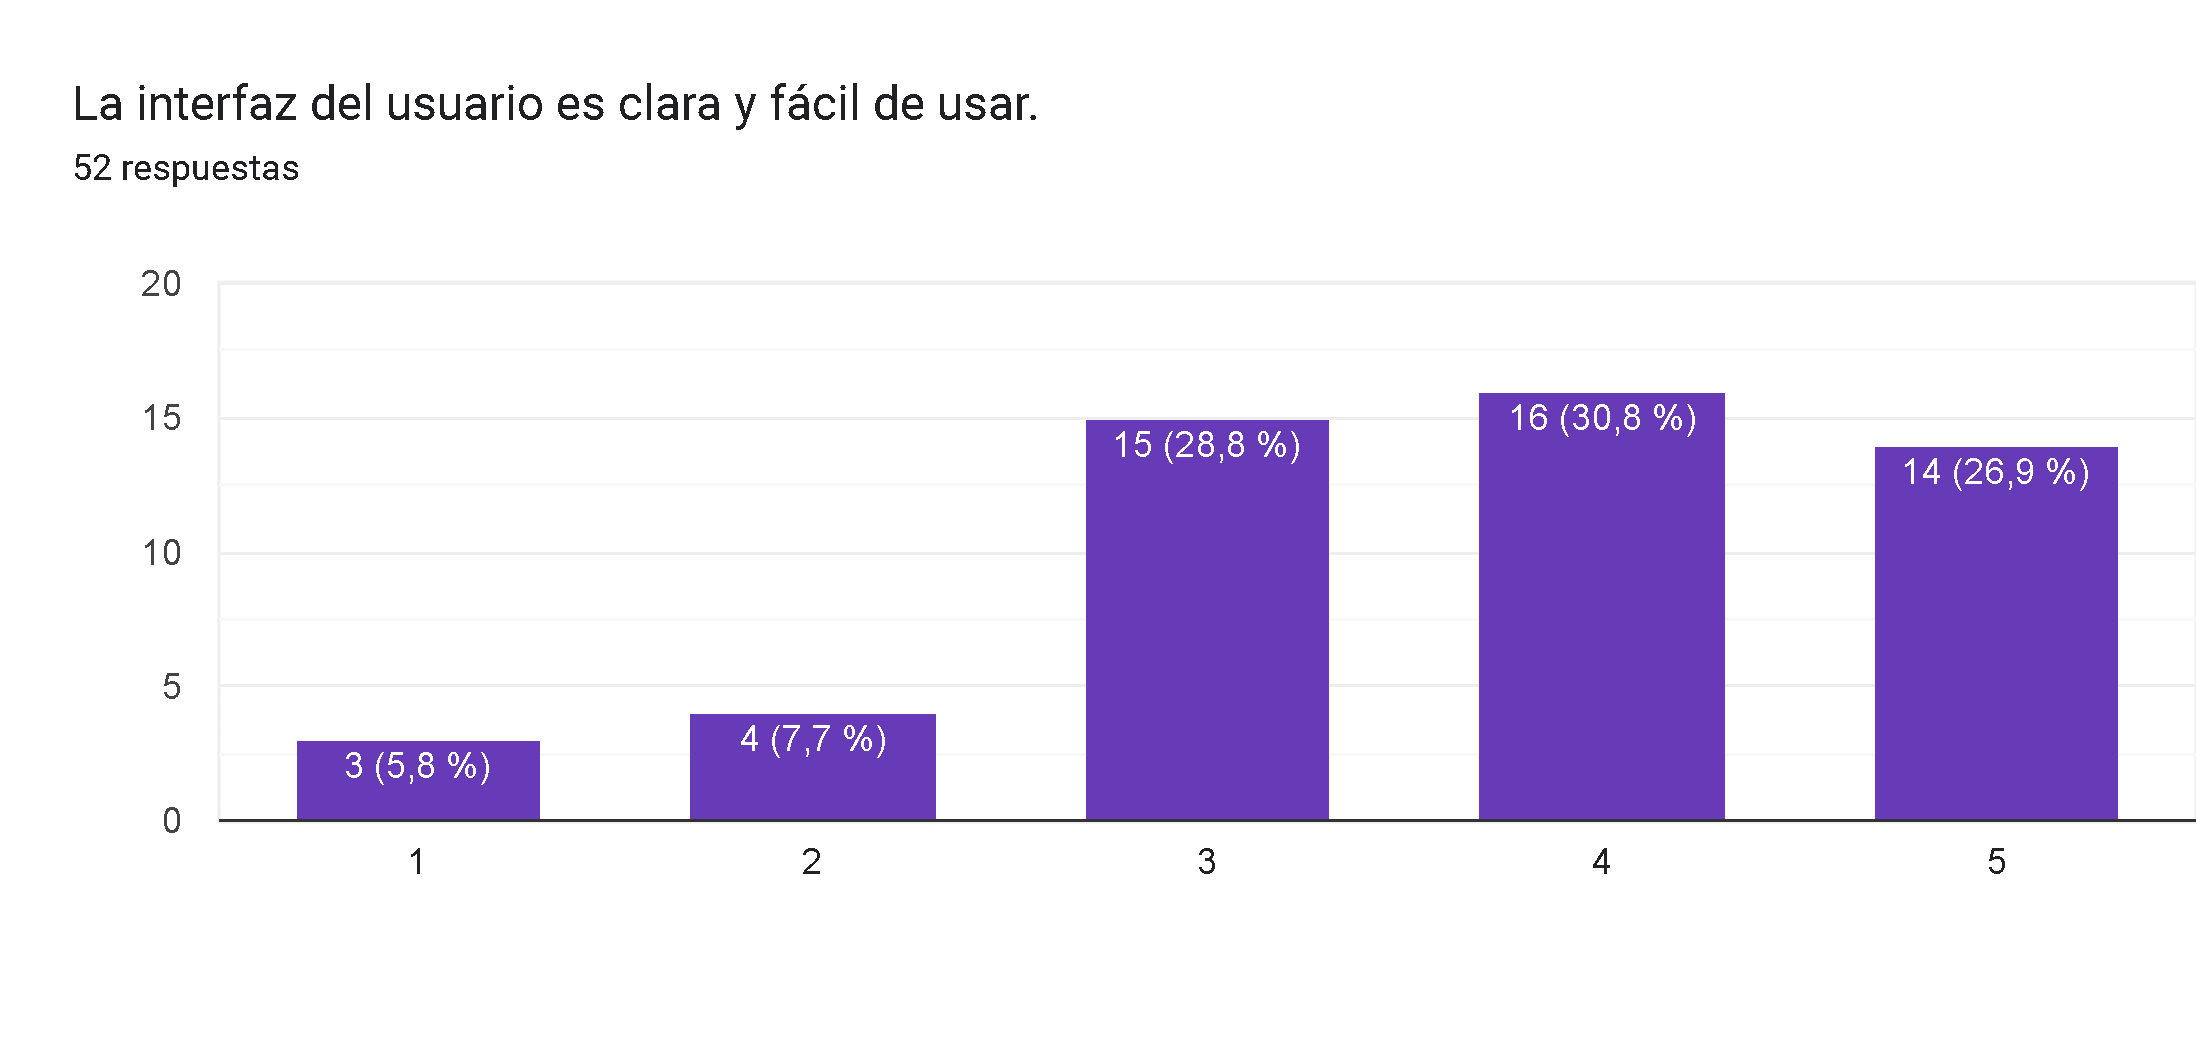
\includegraphics[width=0.7\linewidth]{Imagenes/fc6.png}
  \caption{Elaboración propia, Módulo fitness, Imagen de referencia sobre cuestionario  de gamificación para el módulo fitness del juego sobre la muñeca, ``La interfaz del usuario es clara y fácil de usar``}
  \label{fig:cuestionario6fitness}
\end{figure}


La pregunta ``El juego se ejecuta sin problemas de rendimiento (lag, caídas de FPS, etc.)`` obtuvo la mayor cantidad de respuestas en la opción 4, con un 40,4 \%. Esto sugiere que el rendimiento del juego es generalmente adecuado, aunque algunos usuarios podrían experimentar leves inconvenientes con el rendimiento.
    \begin{figure}[H]
  \centering
  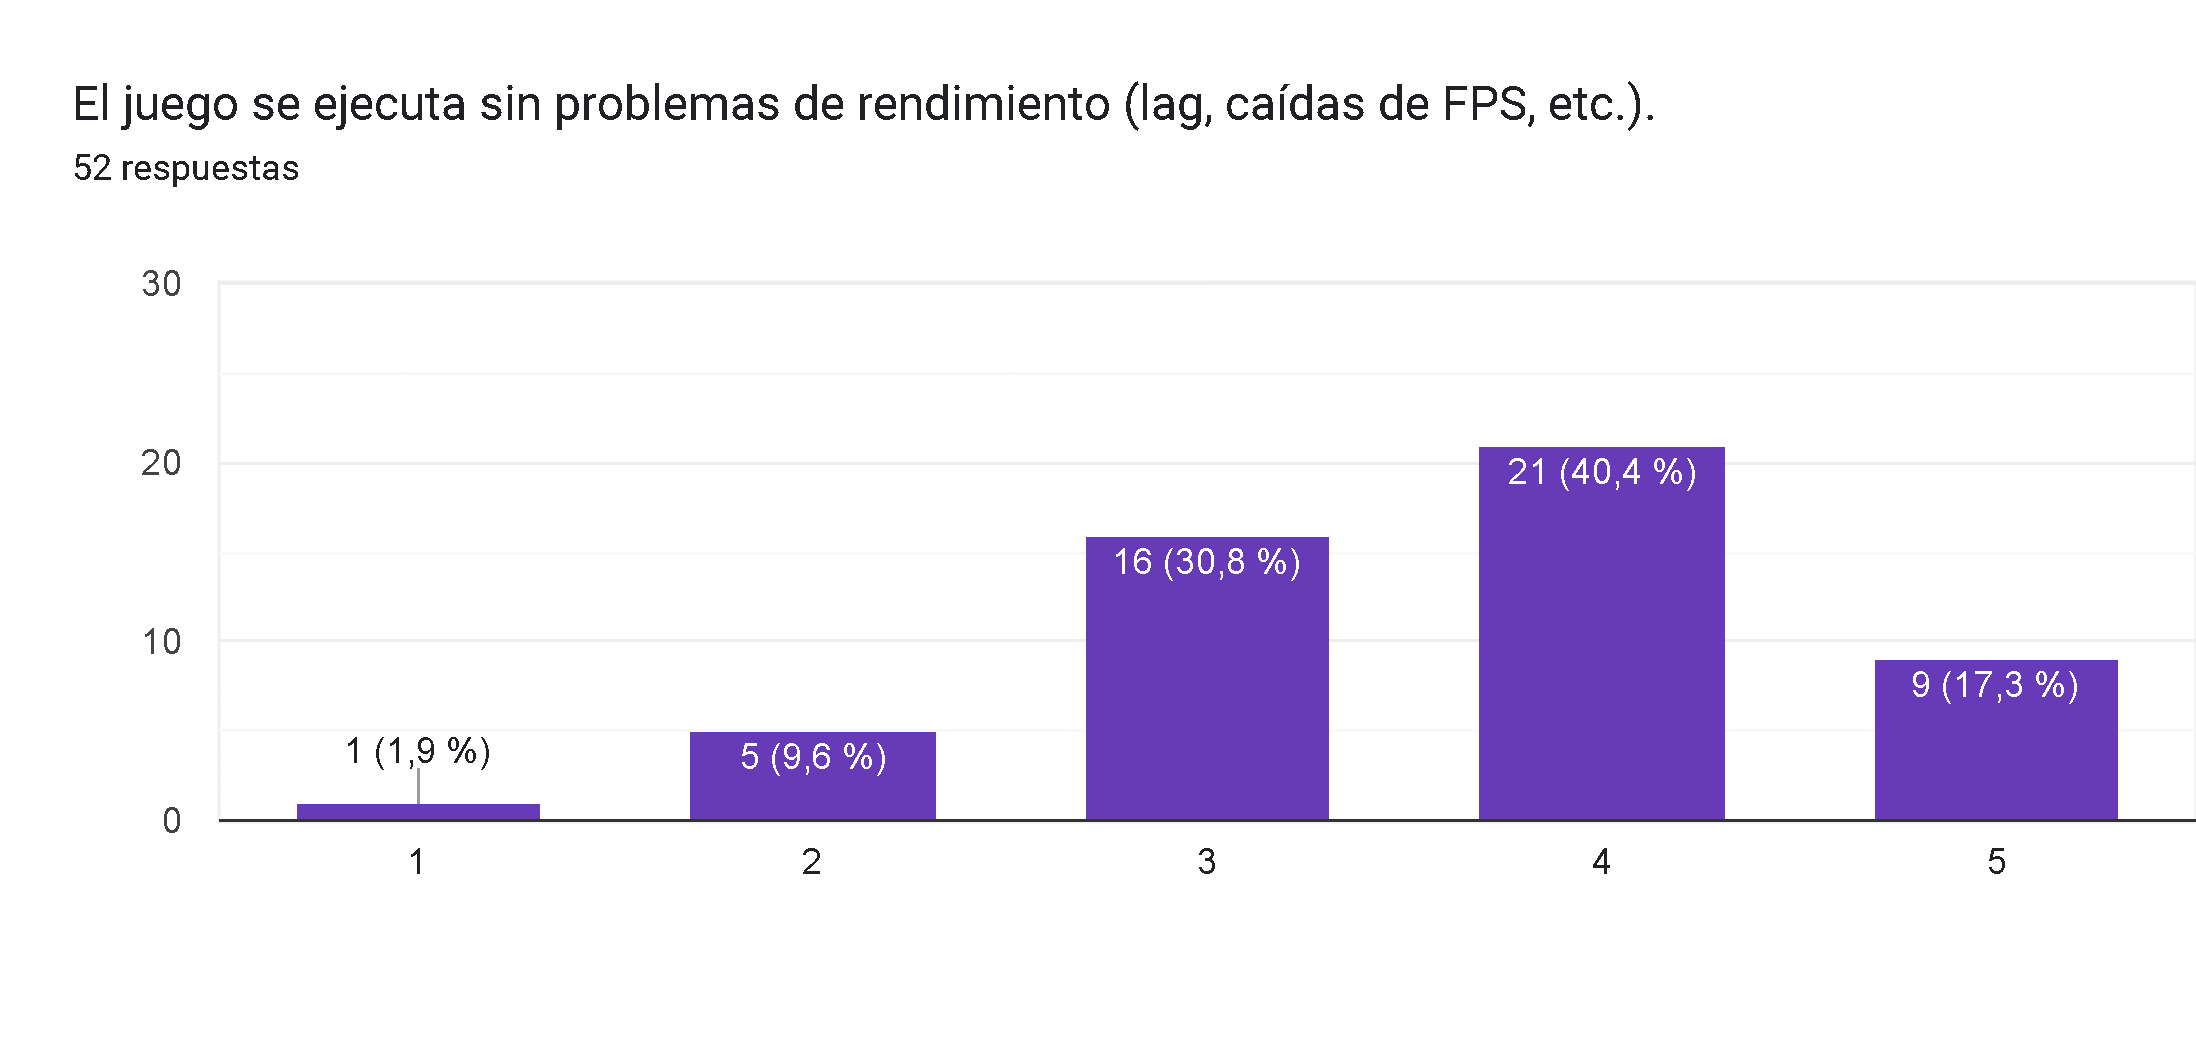
\includegraphics[width=0.7\linewidth]{Imagenes/fc7.png}
  \caption{Elaboración propia, Módulo fitness, Imagen de referencia sobre cuestionario  de gamificación para el módulo fitness del juego sobre la muñeca,``El juego se ejecuta sin problemas de rendimiento (lag, caídas de FPS, etc.)`` }
  \label{fig:cuestionario7fitness}
\end{figure}


La pregunta ``No he experimentado fallos técnicos o bugs importantes`` obtuvo la mayor cantidad de respuestas en la opción 4, con un 51,9 \%. Esto indica que la mayoría de los usuarios no han experimentado problemas técnicos significativos, aunque un porcentaje menor aún podría haber encontrado algunos inconvenientes.

    \begin{figure}[H]
  \centering
  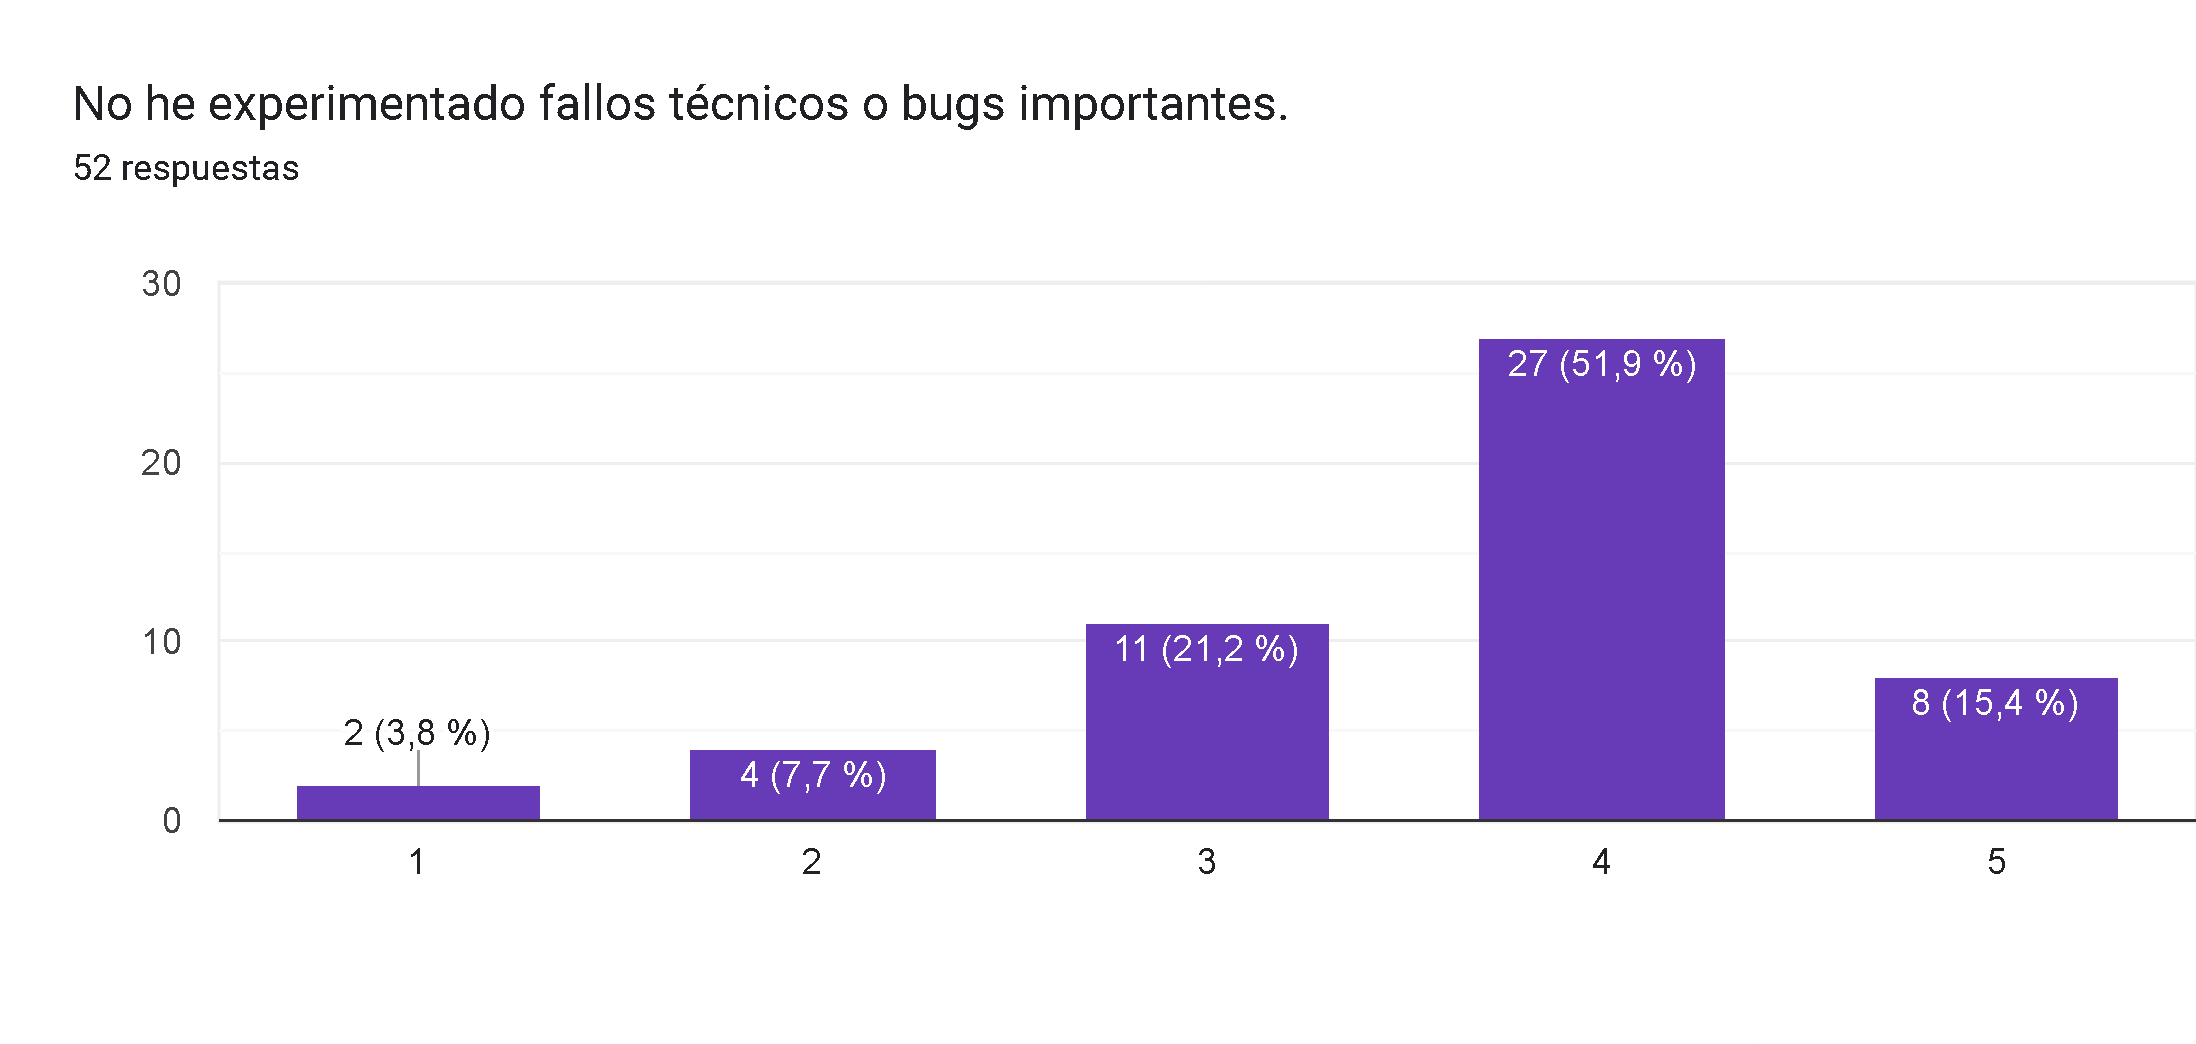
\includegraphics[width=0.7\linewidth]{Imagenes/fc8.png}
  \caption{Elaboración propia, Módulo fitness, Imagen de referencia sobre cuestionario  de gamificación para el módulo fitness del juego sobre la muñeca,``No he experimentado fallos técnicos o bugs importantes``}
  \label{fig:cuestionario8fitness}
\end{figure}

La pregunta ``El juego me ha mantenido motivado para seguir jugando`` obtuvo la misma cantidad de respuestas en las opciones 4 y 3, con un 30,8 \% en ambas. Esto sugiere que la motivación del jugador varía, con una parte significativa encontrando el juego suficientemente motivador, mientras que otros podrían necesitar más incentivos para seguir jugando.

    \begin{figure}[H]
  \centering
  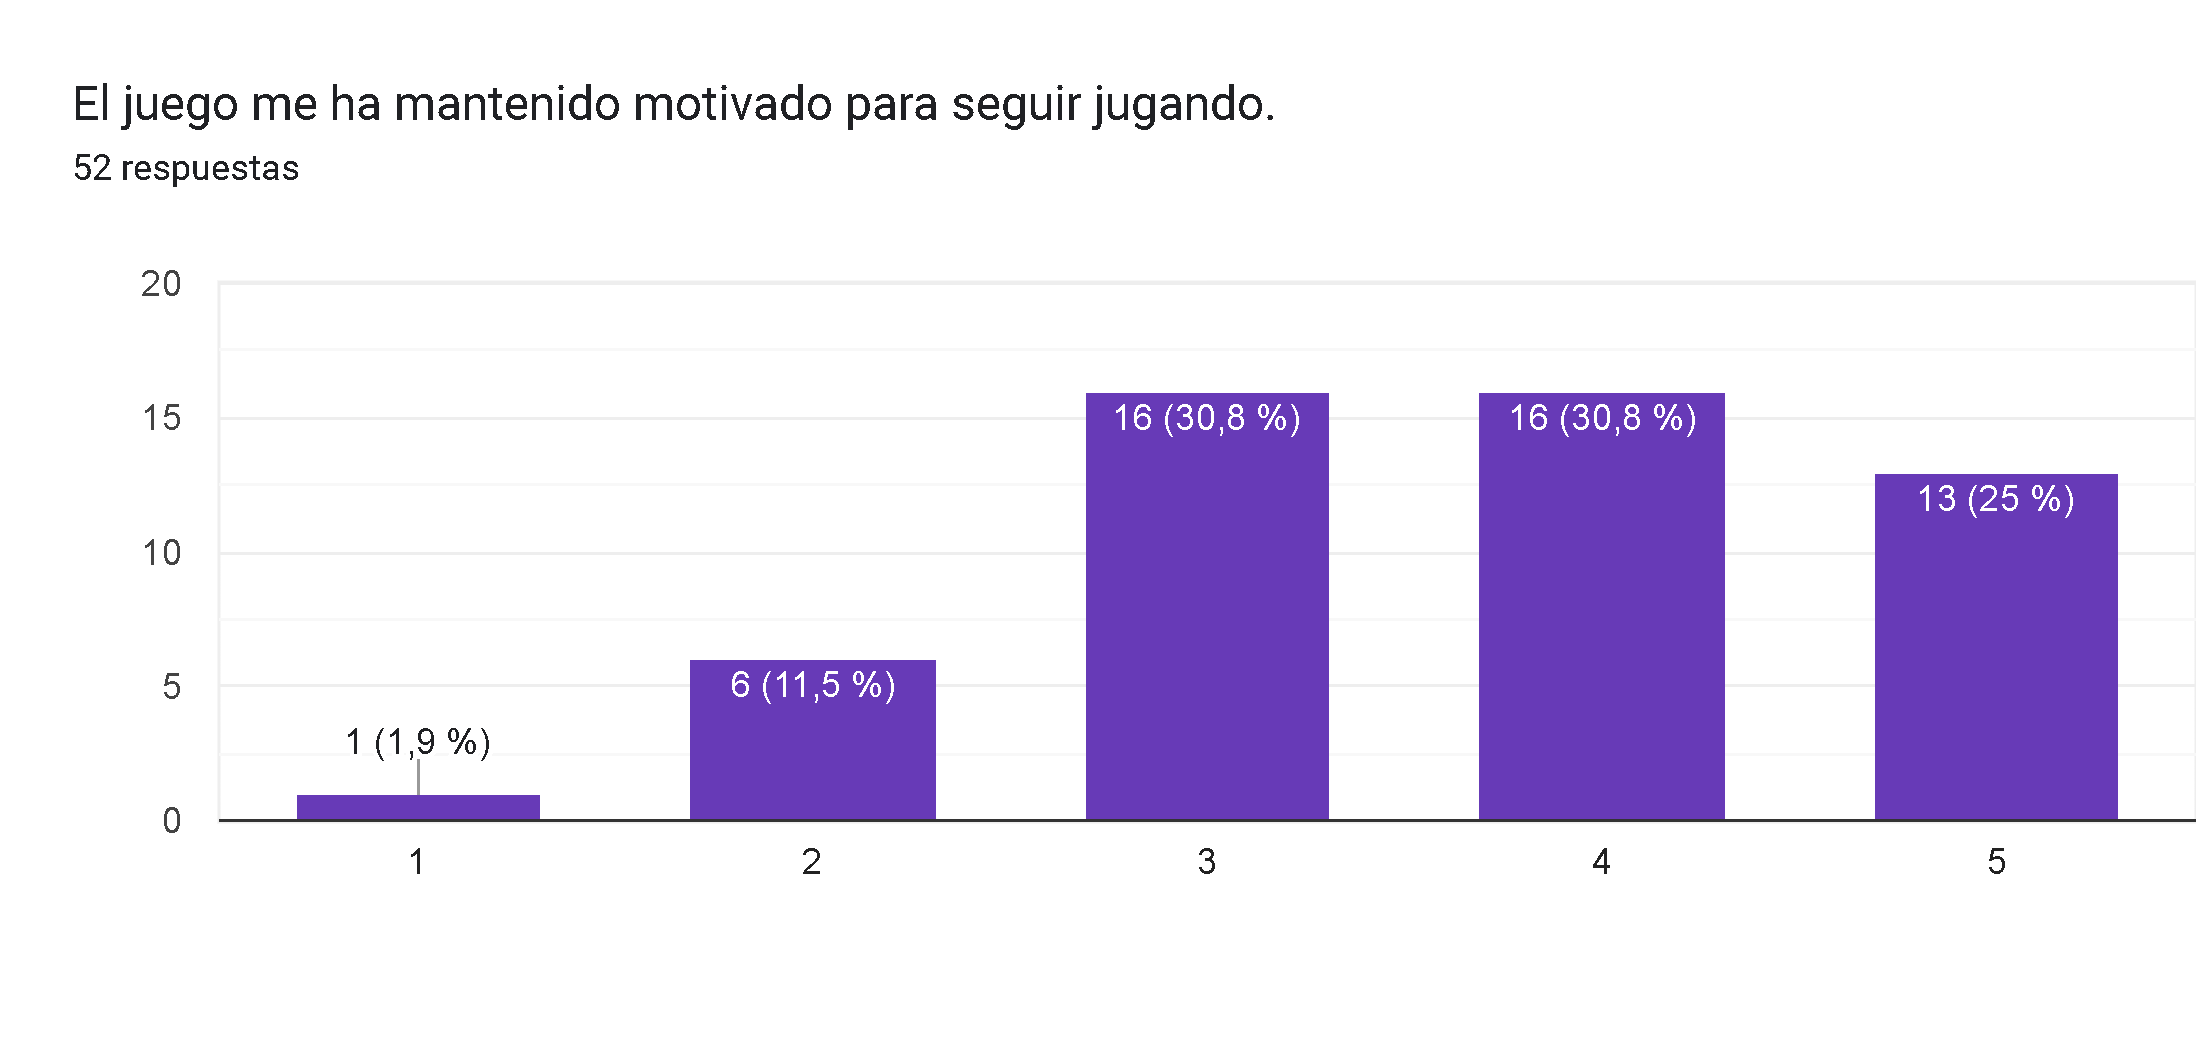
\includegraphics[width=0.7\linewidth]{Imagenes/fc9.png}
  \caption{Elaboración propia, Módulo fitness, Imagen de referencia sobre cuestionario  de gamificación para el módulo fitness del juego sobre la muñeca,``El juego me ha mantenido motivado para seguir jugando`` }
  \label{fig:cuestionario9fitness}
\end{figure}


La pregunta ``Me siento satisfecho con la experiencia general del juego`` obtuvo la mayor cantidad de respuestas en la opción 4, con un 44,2 \%. Esto sugiere que la mayoría de los usuarios están satisfechos con la experiencia general, aunque algunos todavía pueden encontrar áreas para mejorar.

    \begin{figure}[H]
  \centering
  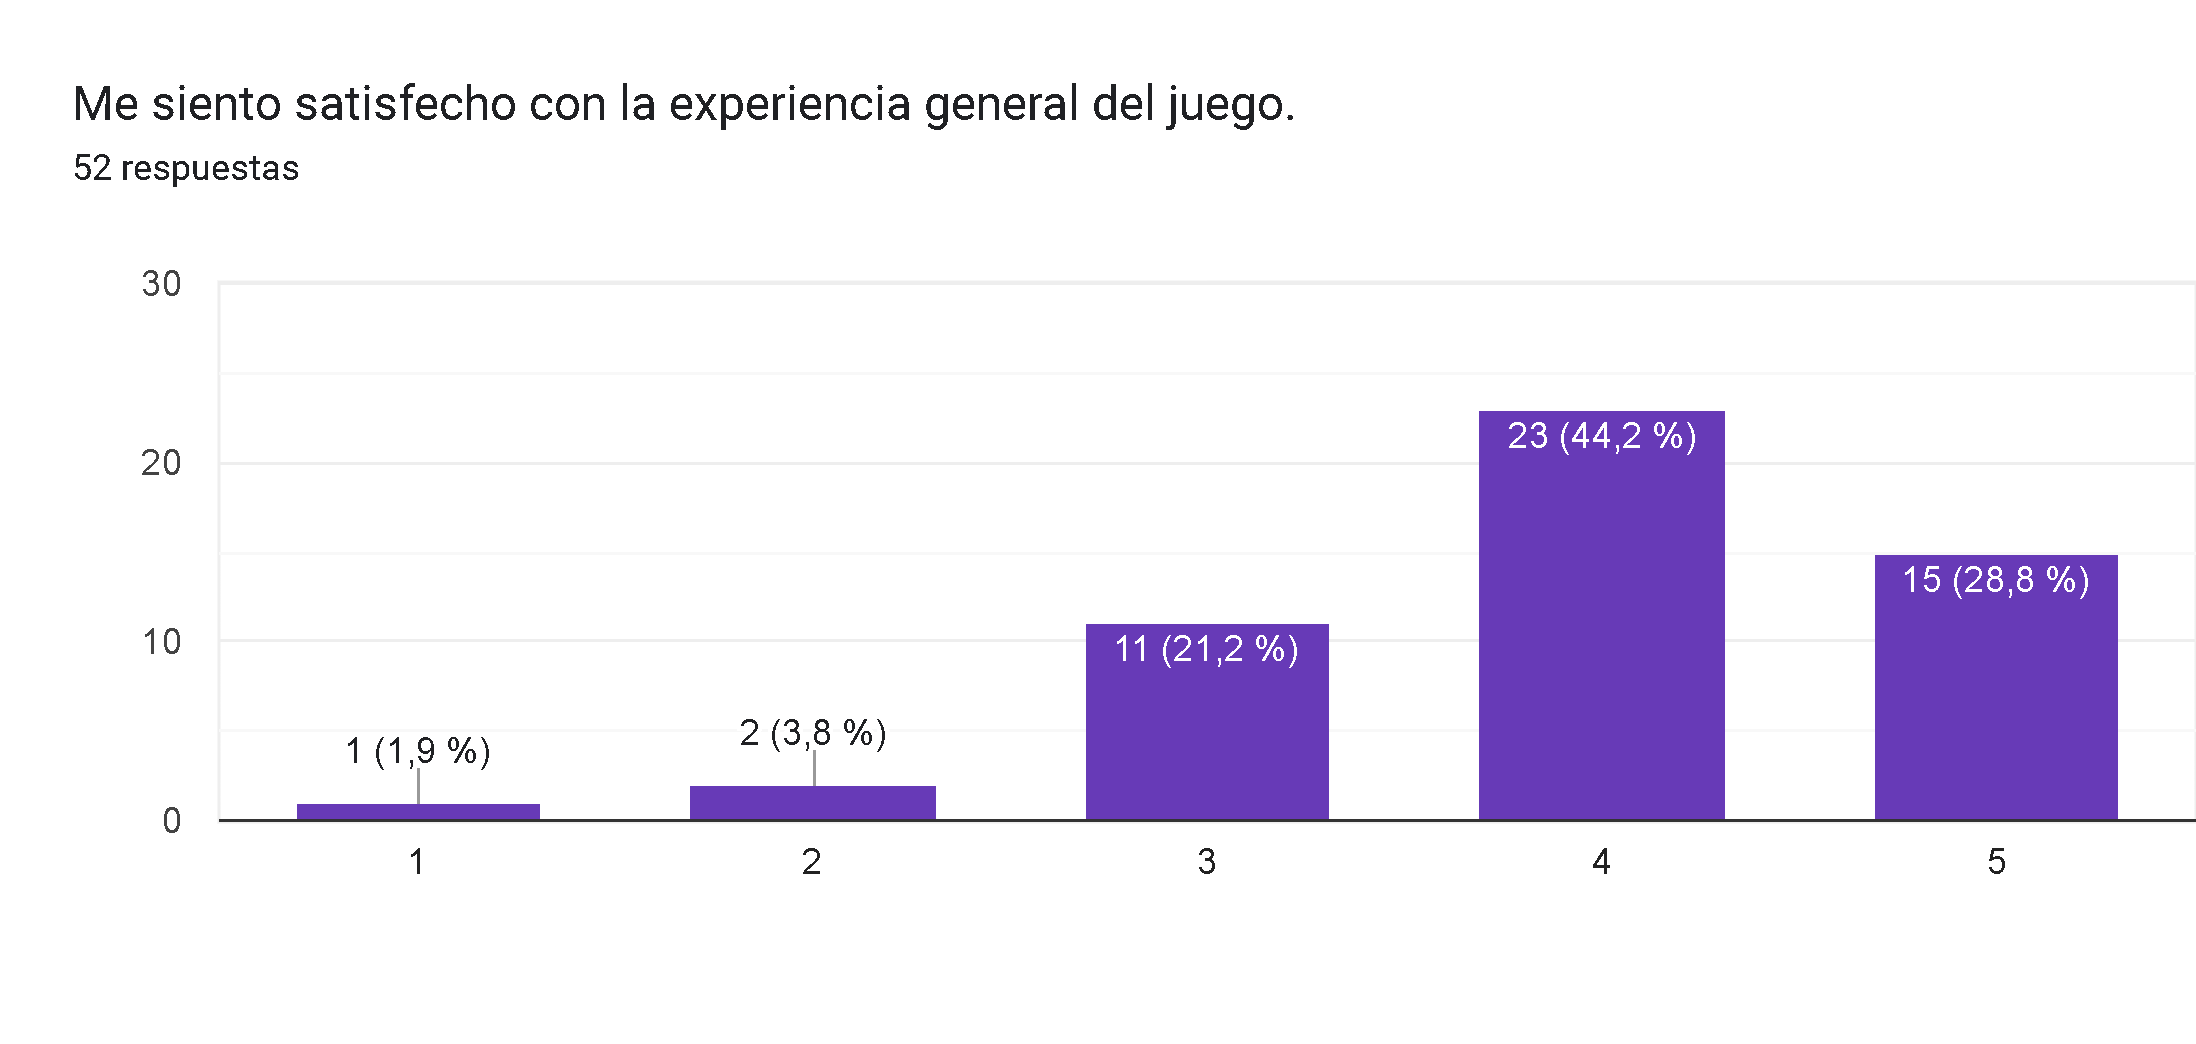
\includegraphics[width=0.7\linewidth]{Imagenes/fc10.png}
  \caption{Elaboración propia, Módulo fitness, Imagen de referencia sobre cuestionario  de gamificación para el módulo fitness del juego sobre la muñeca,``Me siento satisfecho con la experiencia general del juego``}
  \label{fig:cuestionario10fitness}
\end{figure}

La pregunta ``Consideras que el juego es útil para ayudar a la prevención del túnel carpiano`` obtuvo la mayor cantidad de respuestas en la opción 4, con un 38,5 \%. Además, un 19,2 \% eligió la opción 3, lo que indica que una parte significativa de los usuarios considera que el juego puede ser útil para la prevención del túnel carpiano, aunque una proporción considerable aún no está completamente segura de su efectividad.


    \begin{figure}[H]
  \centering
  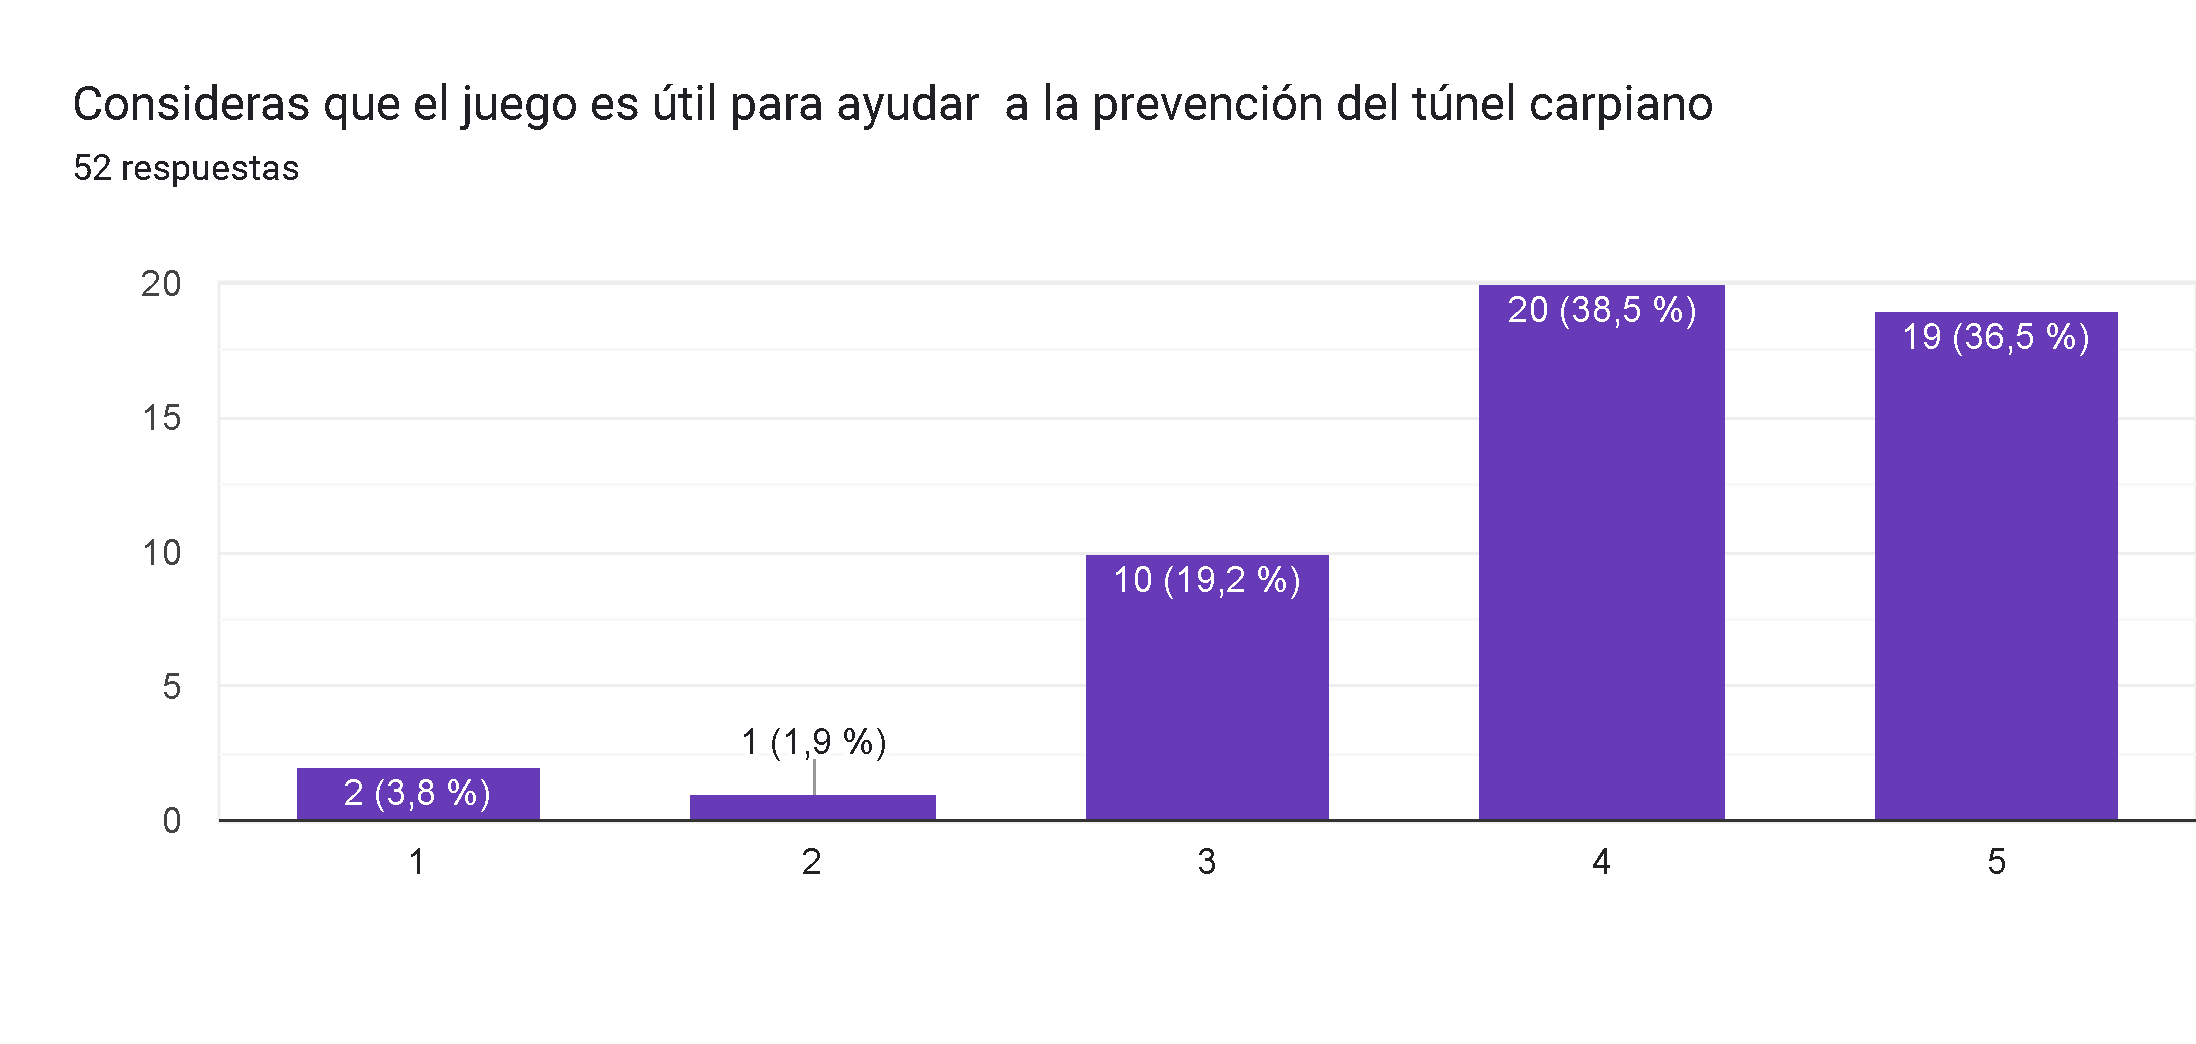
\includegraphics[width=0.7\linewidth]{Imagenes/fc11.png}
  \caption{Elaboración propia, Módulo fitness, Imagen de referencia sobre cuestionario  de gamificación para el módulo fitness del juego sobre la muñeca,``Consideras que el juego es útil para ayudar a la prevención del túnel carpiano``  }
  \label{fig:cuestionario11fitness}
\end{figure}



\subsection{Fitness: Juego sobre movimiento de la espalda}
La pregunta ``El juego es fácil de entender y aprender`` obtuvo la mayor cantidad de respuestas en la opción 4, con un 41,2 \%. Esto indica que la mayoría de los usuarios consideran que el juego es comprensible y fácil de aprender, aunque una parte también encuentra áreas que podrían mejorarse para facilitar aún más su comprensión.

\begin{figure}[H]
  \centering
  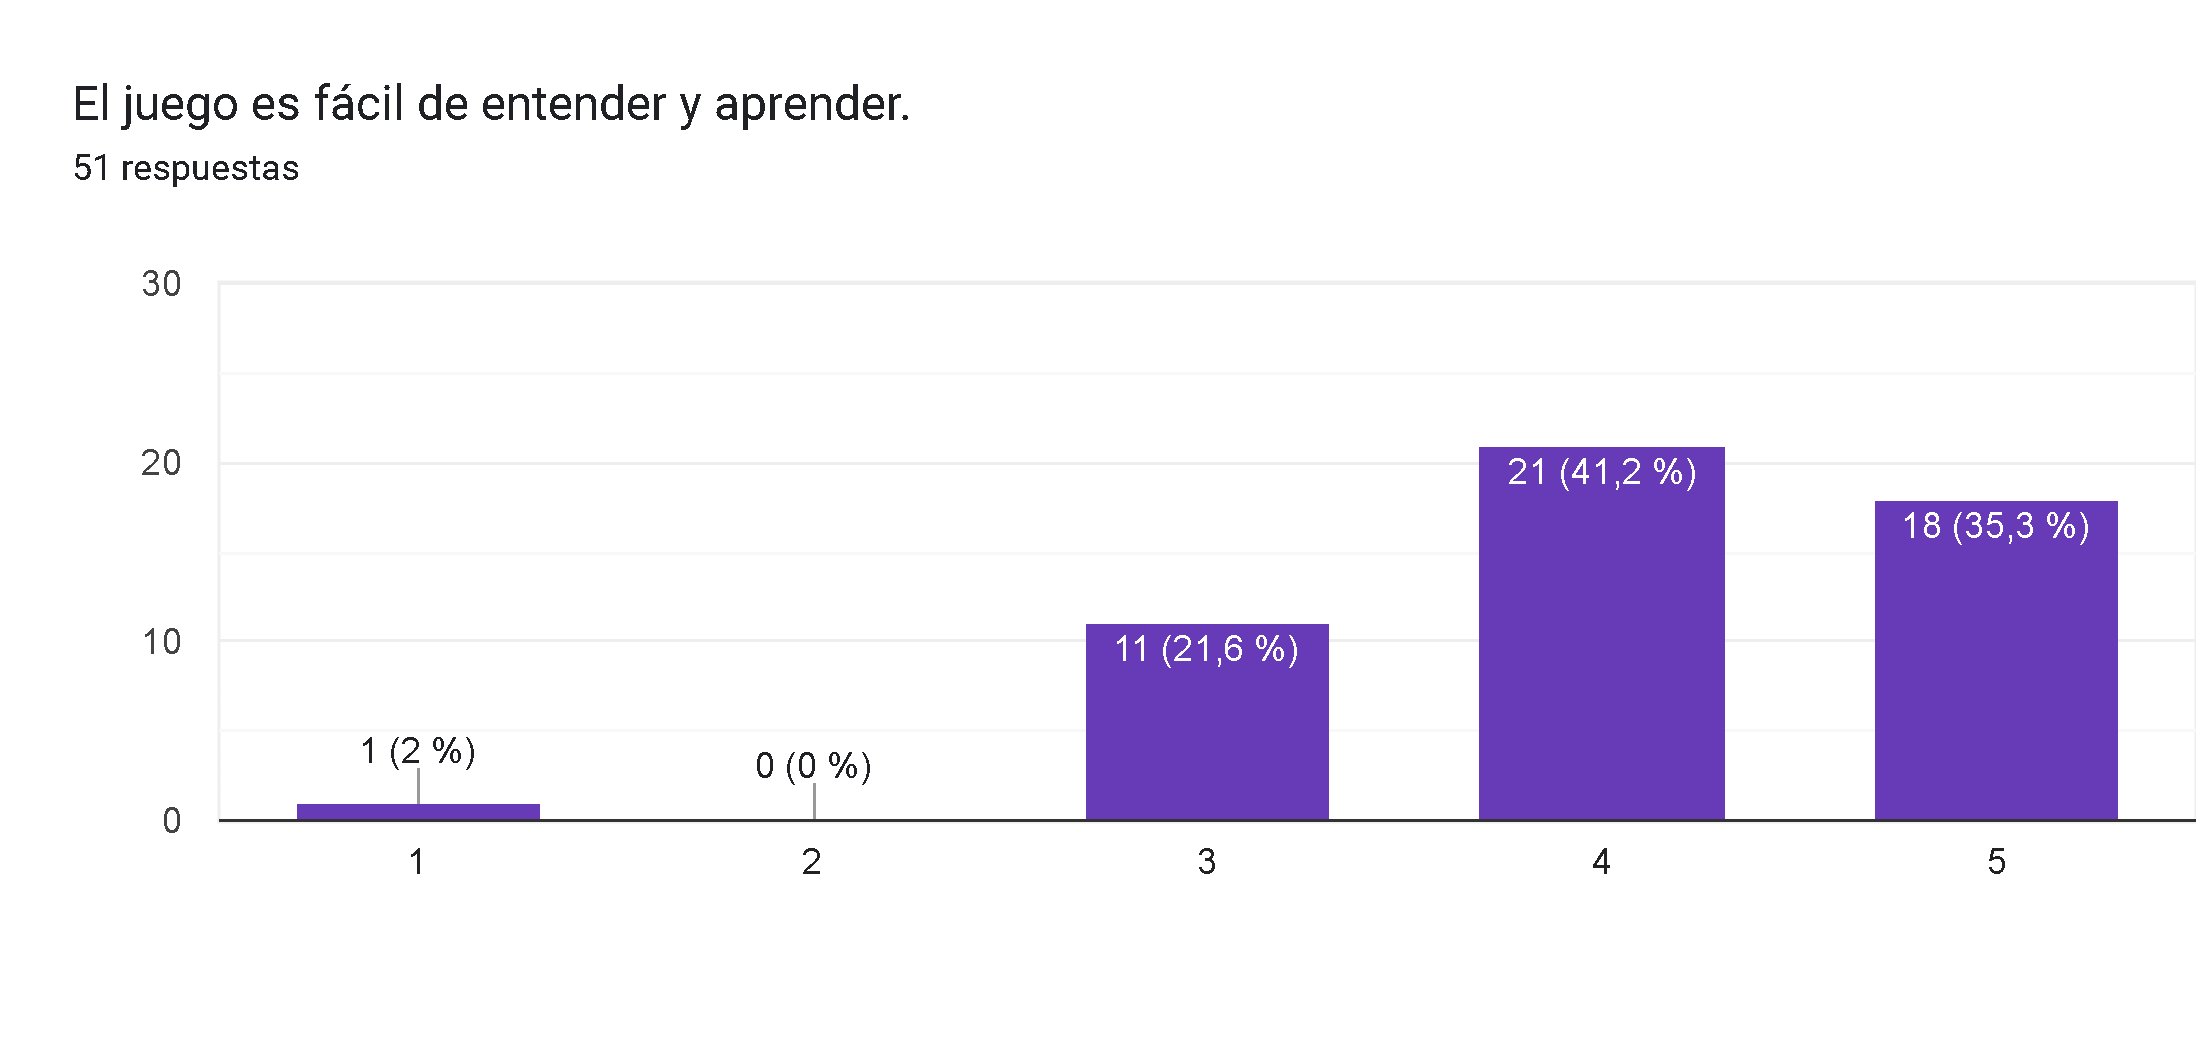
\includegraphics[width=0.7\linewidth]{Imagenes/fd1.png}
  \caption{Elaboración propia, Módulo fitness, Imagen de referencia sobre cuestionario de gamificación para el módulo fitness del juego sobre el movimiento de la espalda, ``El juego es fácil de entender y aprender``}
  \label{fig:cuestionario12fitness}
\end{figure}


La pregunta ``Los controles son intuitivos y responden bien`` obtuvo 24 respuestas en la opción 4, con una mayoría de opiniones positivas. Esto sugiere que los sensores para indicar la posición de la espalda funcionan de manera adecuada, brindando una experiencia satisfactoria a los usuarios.

\begin{figure}[H]
  \centering
  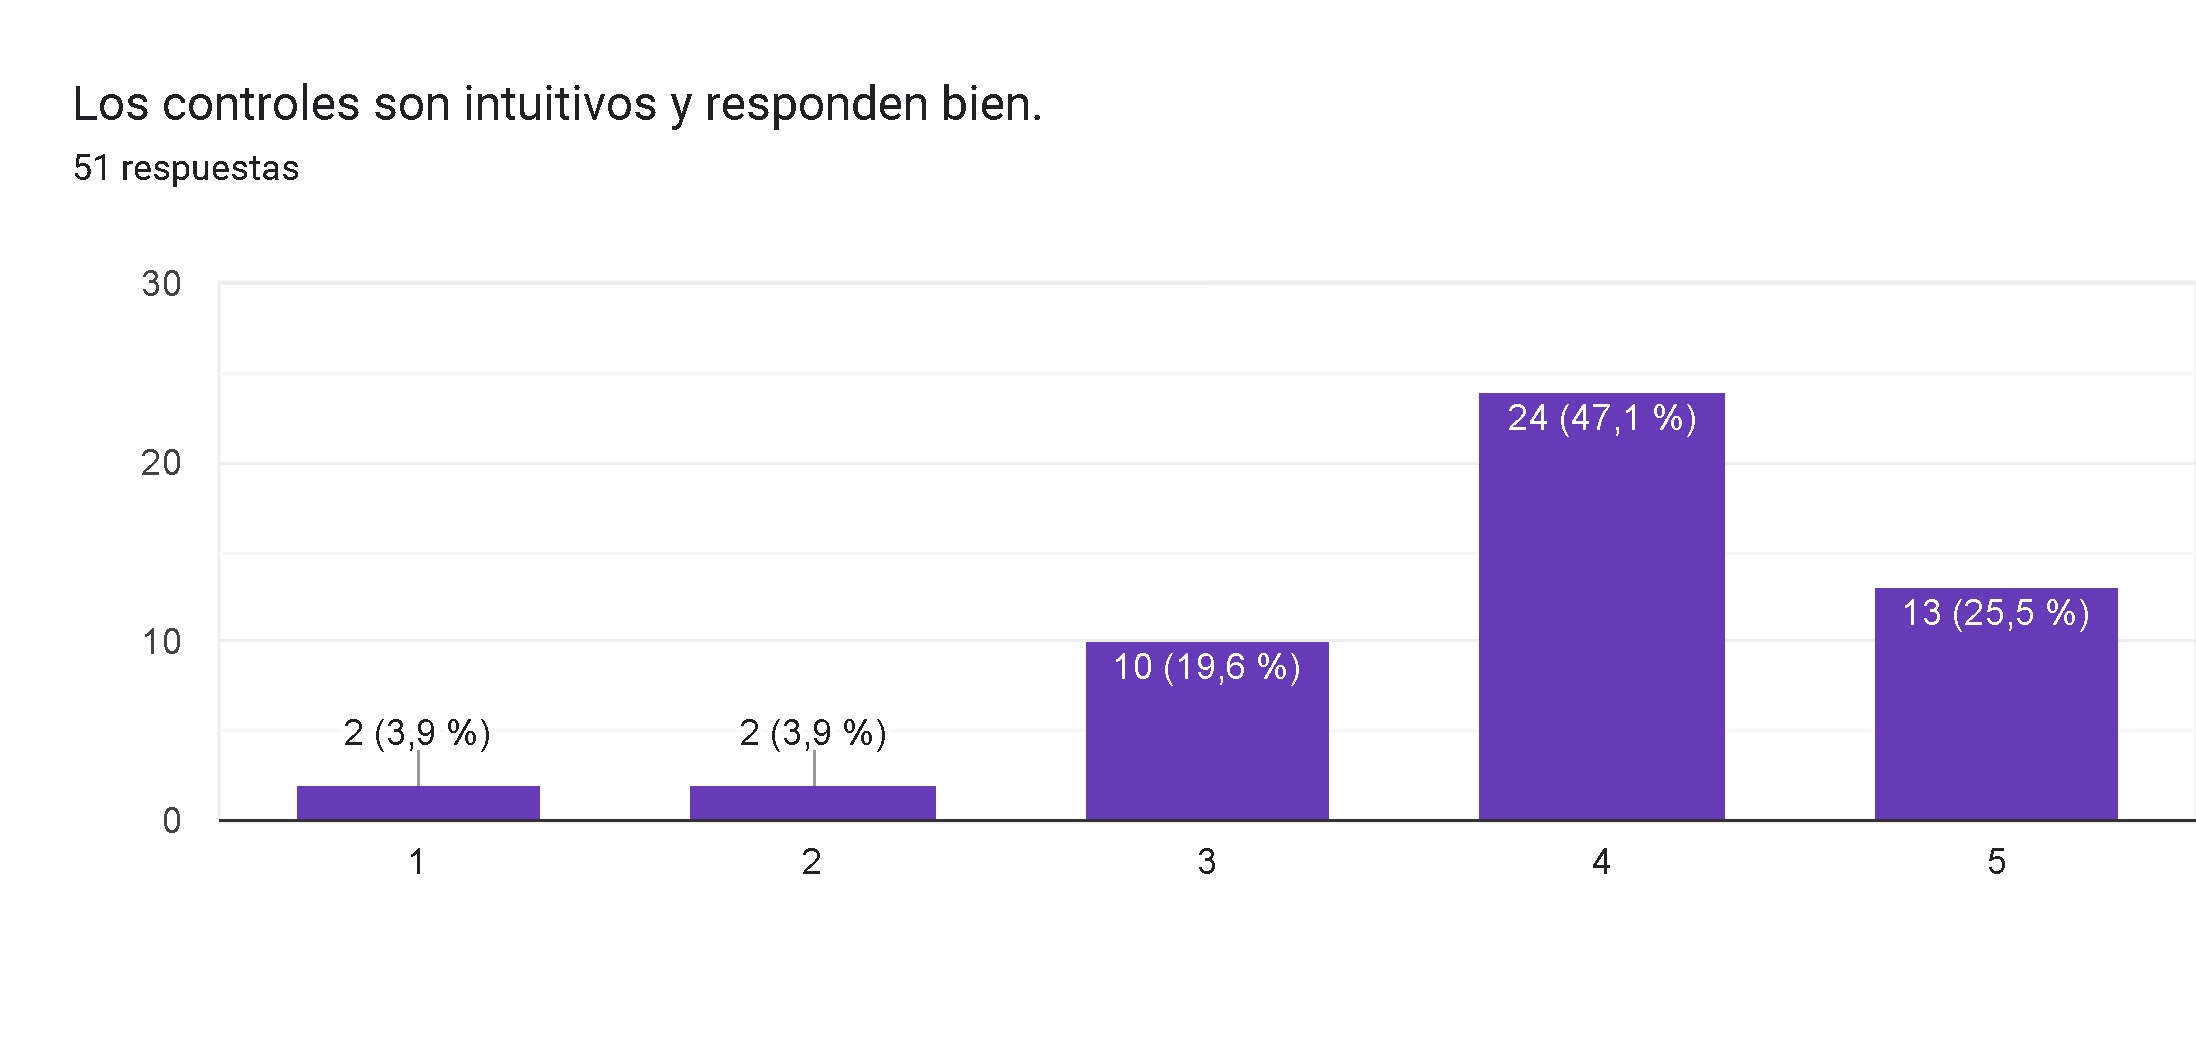
\includegraphics[width=0.7\linewidth]{Imagenes/fd2.png}
  \caption{Elaboración propia, Módulo fitness, Imagen de referencia sobre cuestionario de gamificación para el módulo fitness del juego sobre el movimiento de la espalda, ``Los controles son intuitivos y responden bien``}
  \label{fig:cuestionario13fitness}
\end{figure}

La pregunta ``El nivel de dificultad es adecuado`` obtuvo la mayor cantidad de respuestas en la opción 4, con un 44,9 \%. Esto sugiere que la mayoría de los usuarios consideran que el nivel de dificultad está bien equilibrado, aunque algunos aún podrían encontrarlo demasiado fácil o desafiante.

\begin{figure}[H]
  \centering
  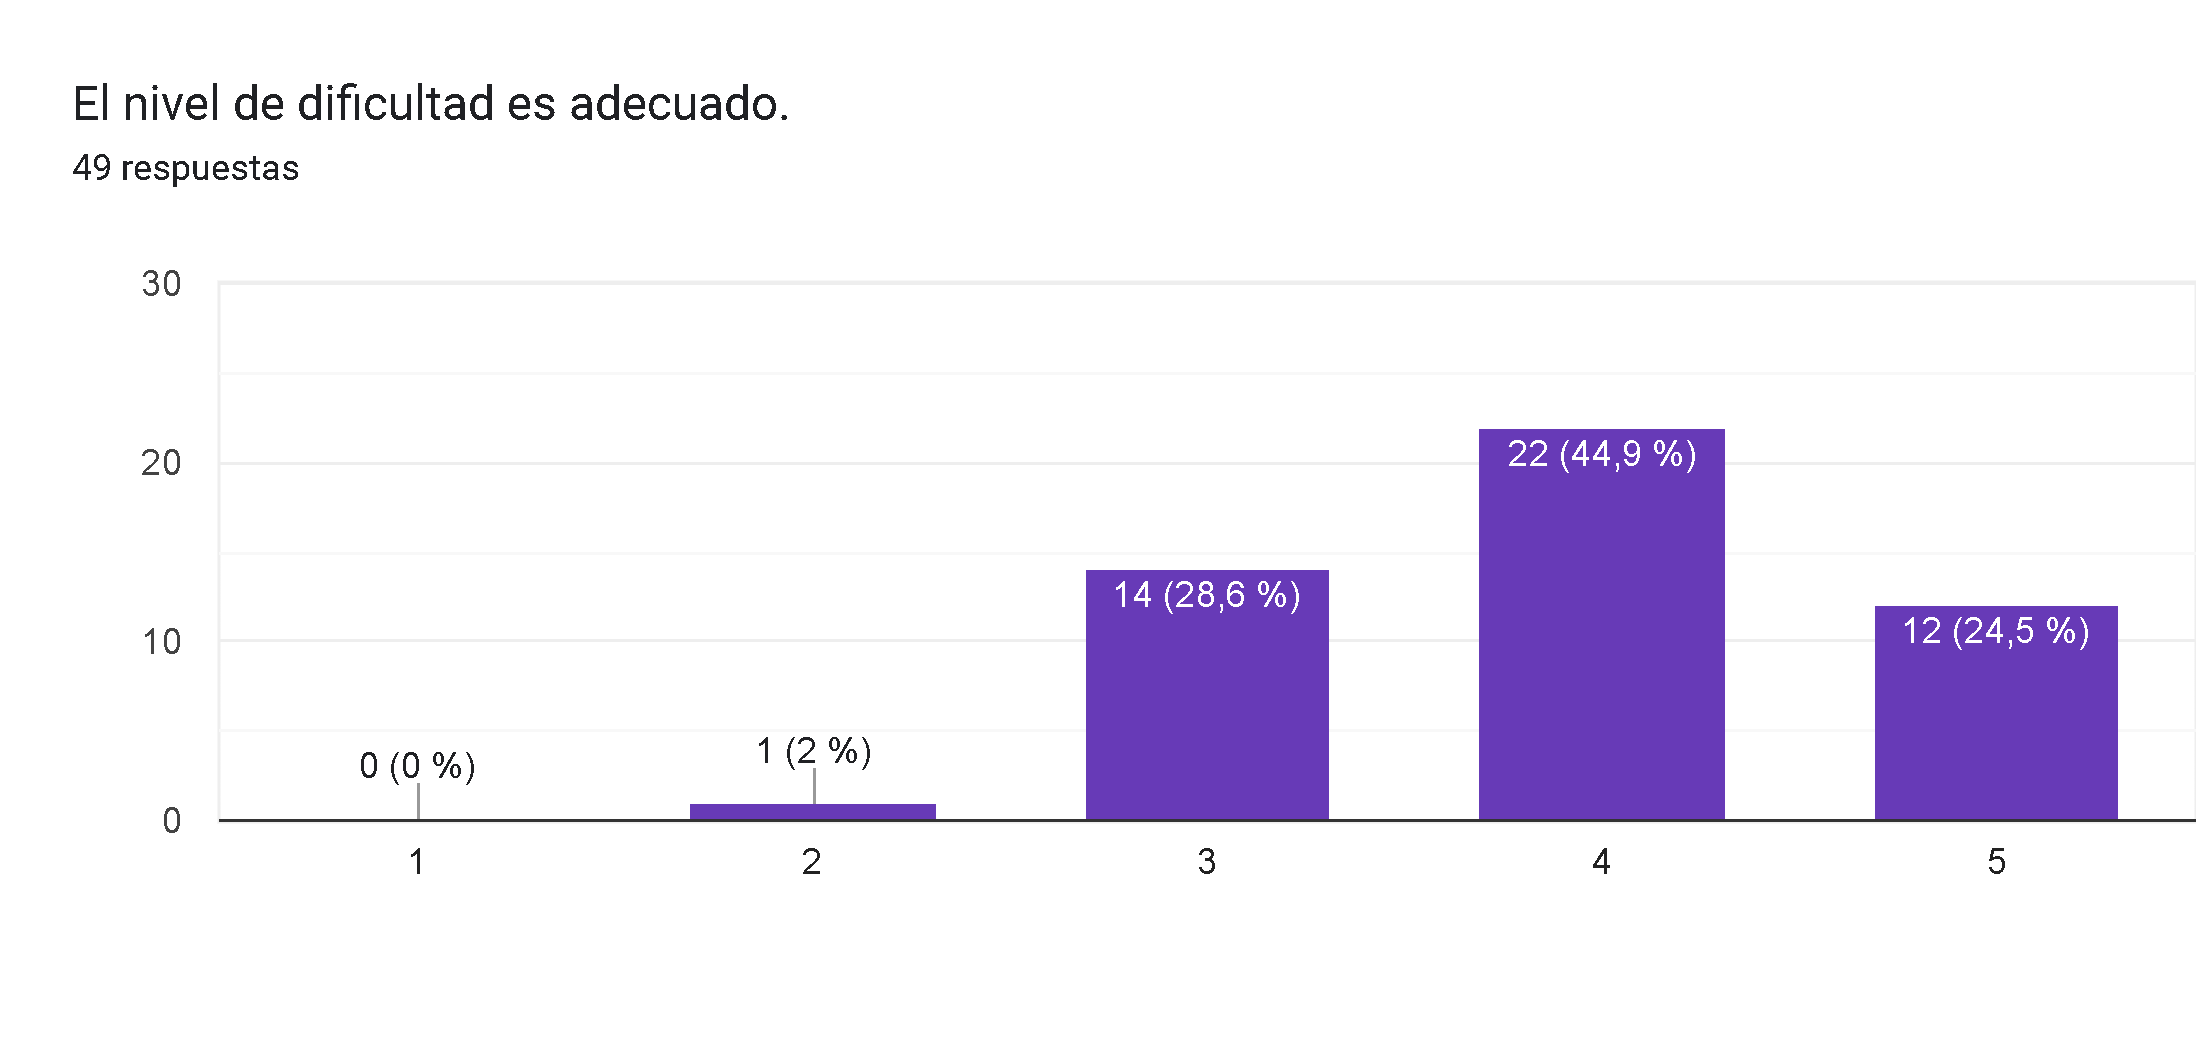
\includegraphics[width=0.7\linewidth]{Imagenes/fd3.png}
  \caption{Elaboración propia, Módulo fitness, Imagen de referencia sobre cuestionario de gamificación para el módulo fitness del juego sobre el movimiento de la espalda, ``El nivel de dificultad es adecuado``}
  \label{fig:cuestionario14fitness}
\end{figure}


La pregunta ``El juego detecta mis movimientos corporales de manera precisa`` obtuvo la mayor cantidad de respuestas en la opción 4, con un 54 \%. Sin embargo, también se observó un 22 \% de respuestas en la opción 3, lo que sugiere que, aunque la mayoría considera que la detección es precisa, hay un porcentaje significativo de usuarios que podrían experimentar dificultades o inconsistencias en la detección.

\begin{figure}[H]
  \centering
  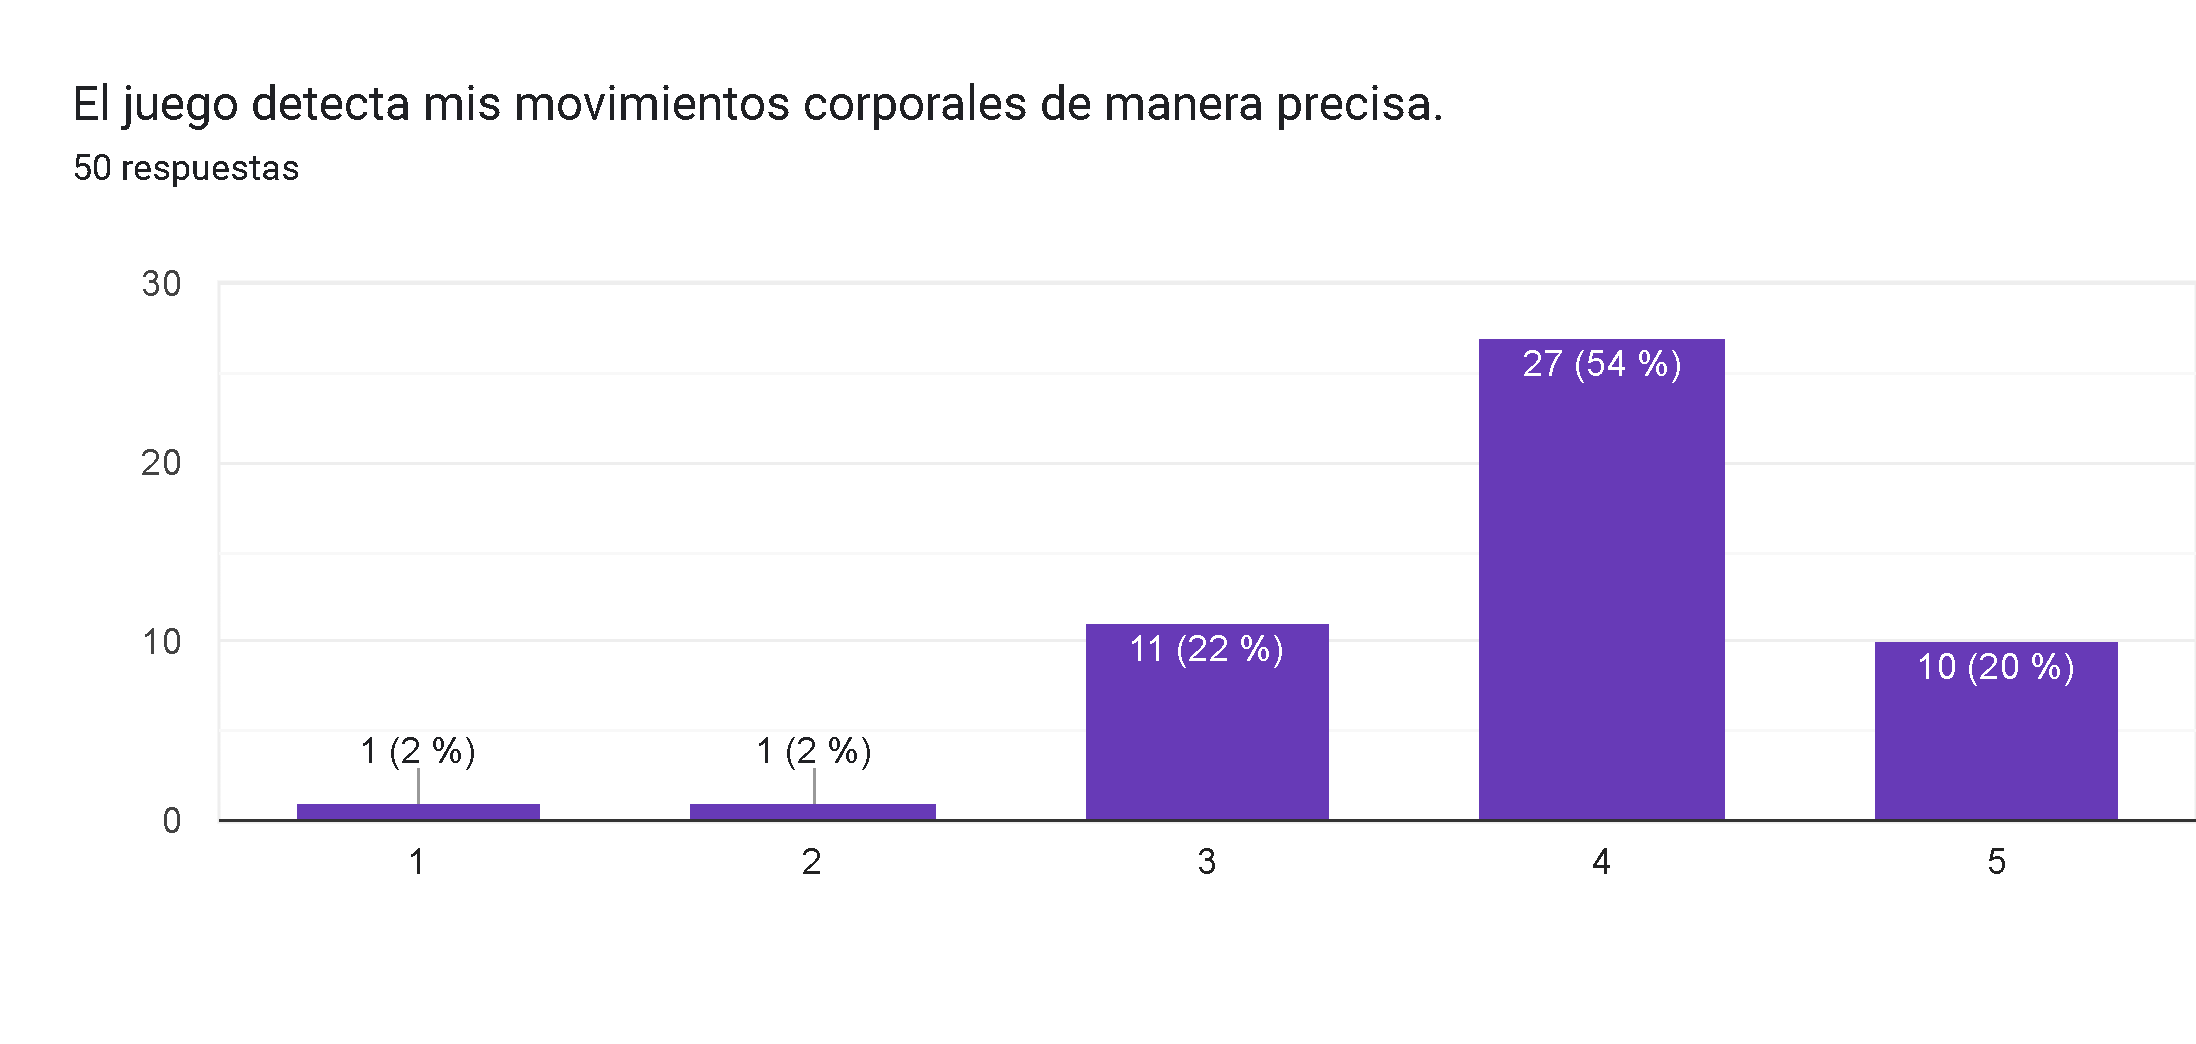
\includegraphics[width=0.7\linewidth]{Imagenes/fd4.png}
  \caption{Elaboración propia, Módulo fitness, Imagen de referencia sobre cuestionario de gamificación para el módulo fitness del juego sobre el movimiento de la espalda, ``El juego detecta mis movimientos corporales de manera precisa``}
  \label{fig:cuestionario15fitness}
\end{figure}

La pregunta ``Los movimientos requeridos no provocan fatiga o molestias físicas`` tuvo una buena recepción, con 22 respuestas en la opción 4. Esto indica que, aparentemente, los movimientos fueron cómodos para los usuarios y no generaron un ambiente incómodo para ellos.

\begin{figure}[H]
  \centering
  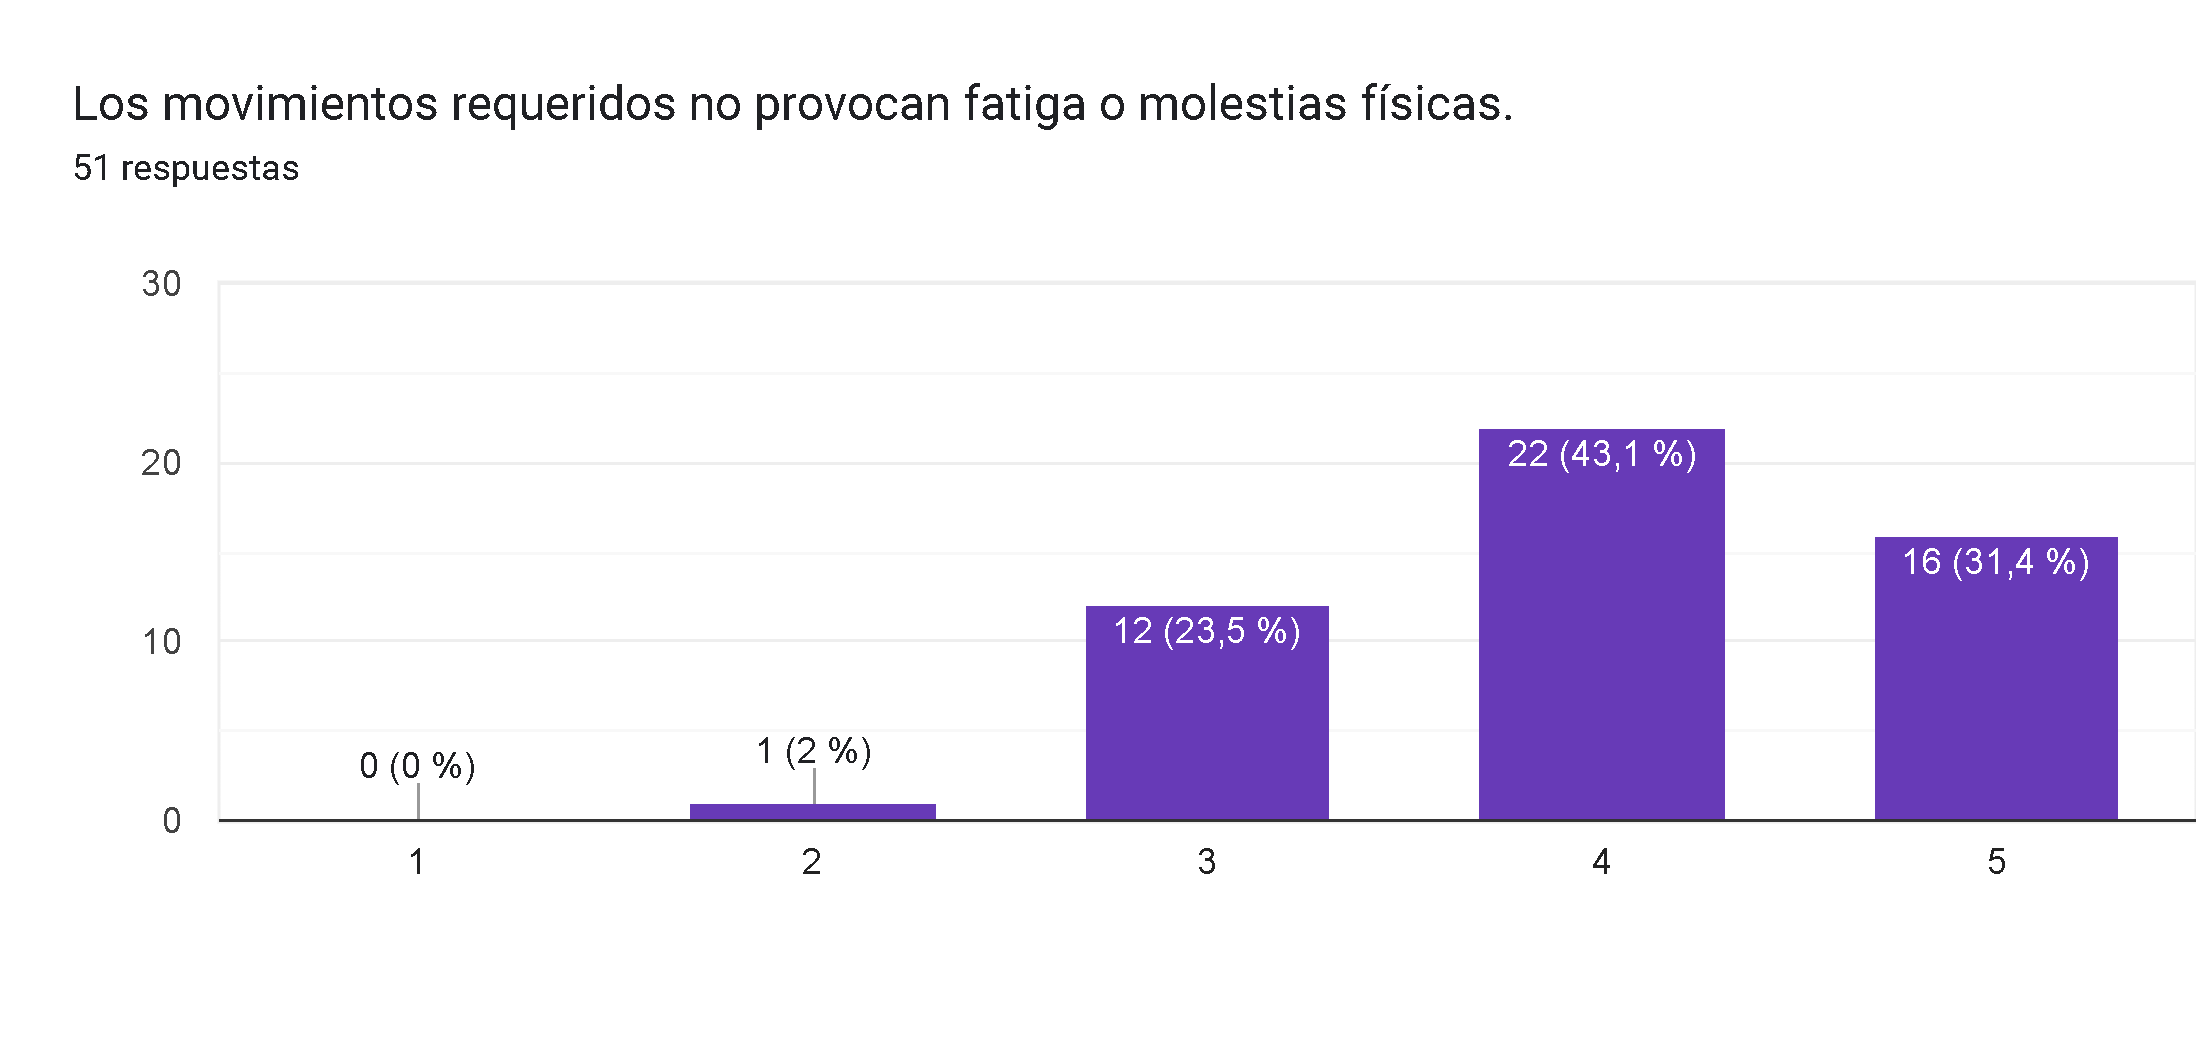
\includegraphics[width=0.7\linewidth]{Imagenes/fd5.png}
  \caption{Elaboración propia, Módulo fitness, Imagen de referencia sobre cuestionario de gamificación para el módulo fitness del juego sobre el movimiento de la espalda, ``Los movimientos requeridos no provocan fatiga o molestias físicas``}
  \label{fig:cuestionario16fitness}
\end{figure}


La pregunta ``La interfaz del usuario es clara y fácil de usar`` obtuvo la mayor cantidad de respuestas en la opción 4, con un 39,2 \%. Además, un 23,5 \% eligió la opción 3, lo que indica que la interfaz es generalmente bien recibida, pero aún hay un grupo significativo que considera que puede mejorarse para ser más clara o accesible.

\begin{figure}[H]
  \centering
  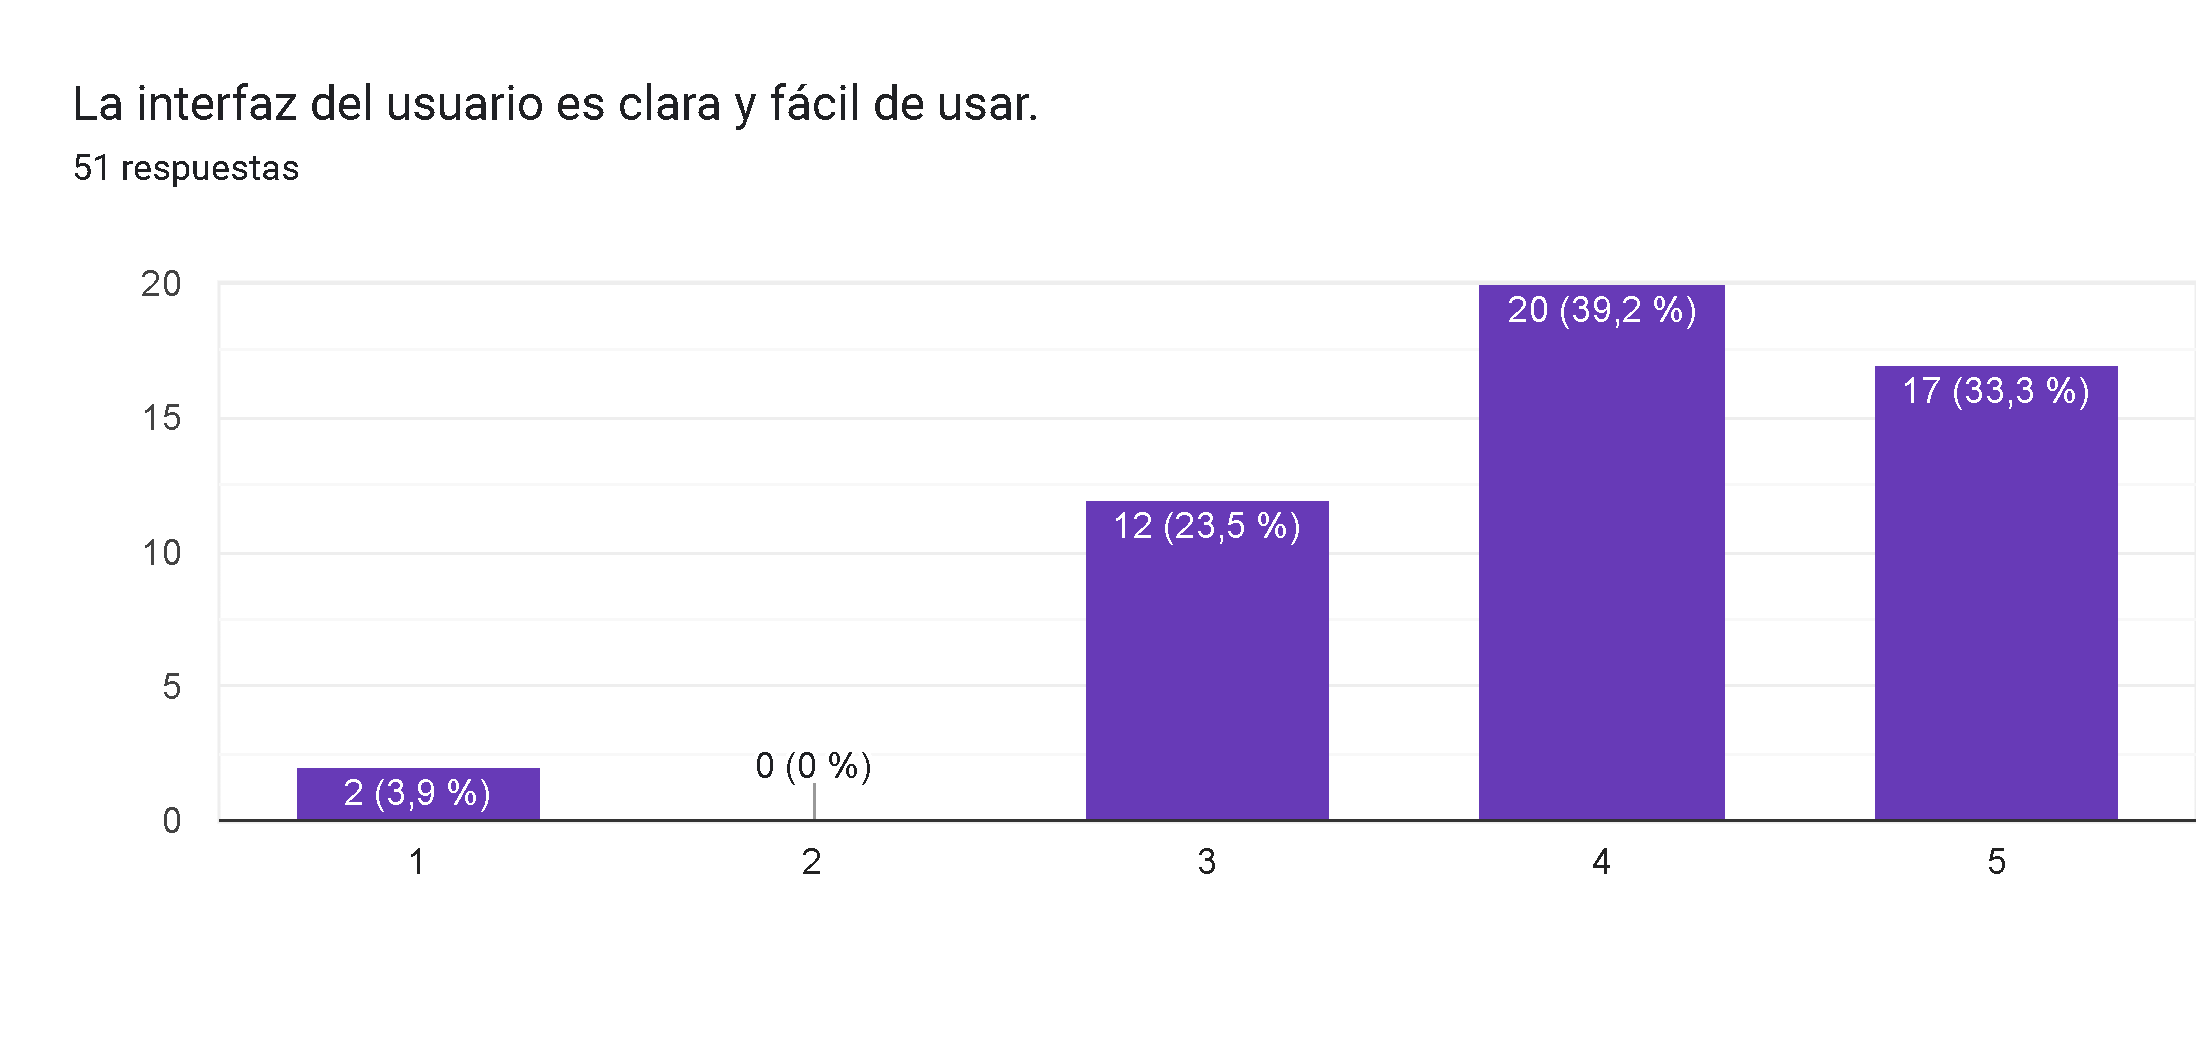
\includegraphics[width=0.7\linewidth]{Imagenes/fd6.png}
  \caption{Elaboración propia, Módulo fitness, Imagen de referencia sobre cuestionario de gamificación para el módulo fitness del juego sobre el movimiento de la espalda, ``La interfaz del usuario es clara y fácil de usar``}
  \label{fig:cuestionario17fitness}
\end{figure}

La pregunta ``La música del juego es adecuada y mejora la experiencia`` tuvo una buena recepción, con la mayoría de las respuestas mayores a 4. Esto indica que, aparentemente, la música fue del agrado de los jugadores y contribuyó positivamente a su experiencia.

\begin{figure}[H]
  \centering
  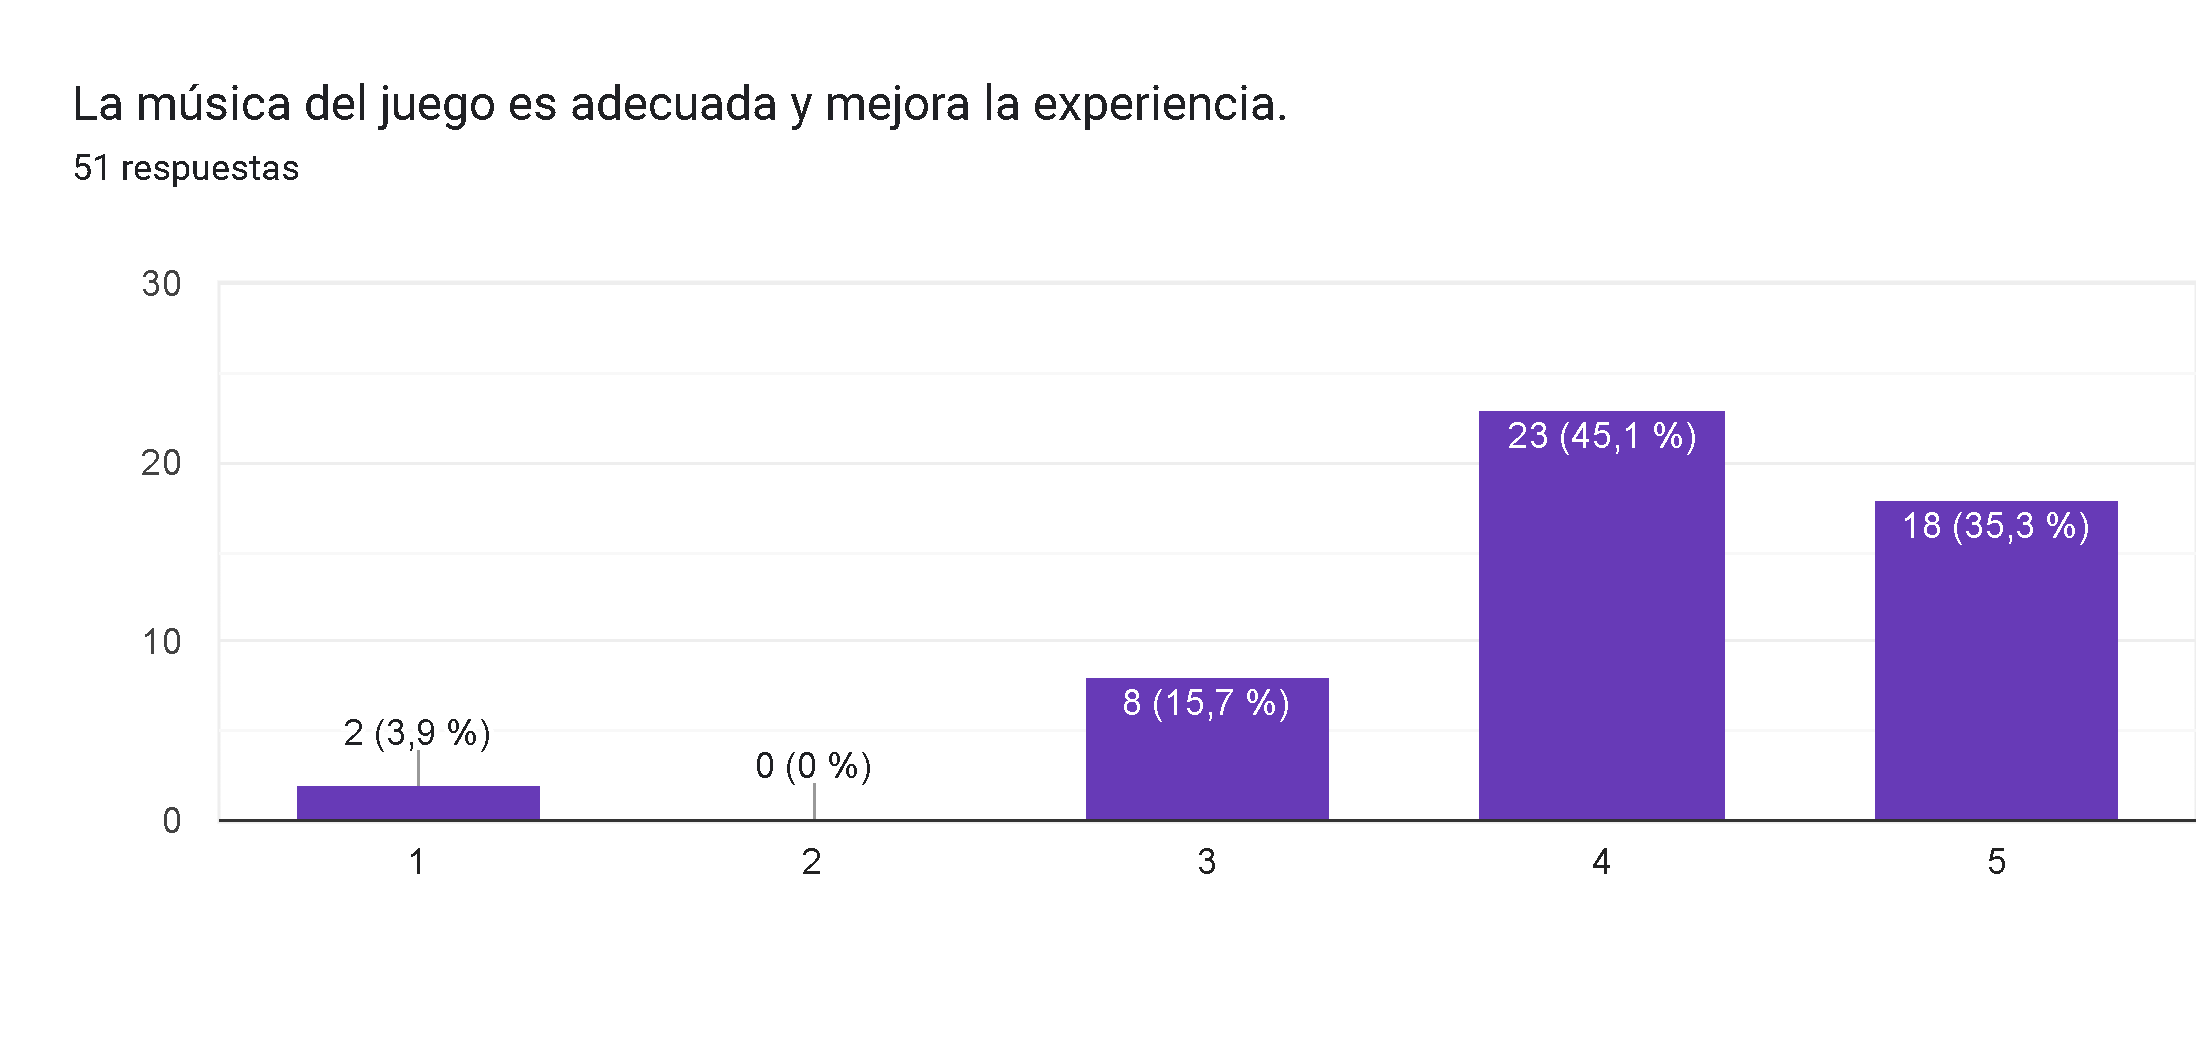
\includegraphics[width=0.7\linewidth]{Imagenes/fd7.png}
  \caption{Elaboración propia, Módulo fitness, Imagen de referencia sobre cuestionario de gamificación para el módulo fitness del juego sobre el movimiento de la espalda, ``La música del juego es adecuada y mejora la experiencia``}
  \label{fig:cuestionario18fitness}
\end{figure}


La pregunta ``El juego se ejecuta sin problemas de rendimiento (lag, caídas de FPS, etc.)`` obtuvo la mayor cantidad de respuestas en la opción 4, con un 41,2 \%. También se observó un 25,5 \% en la opción 3, lo que sugiere que la mayoría de los usuarios experimenta un buen rendimiento, aunque un grupo considerable podría haber notado leves problemas en el rendimiento.

\begin{figure}[H]
  \centering
  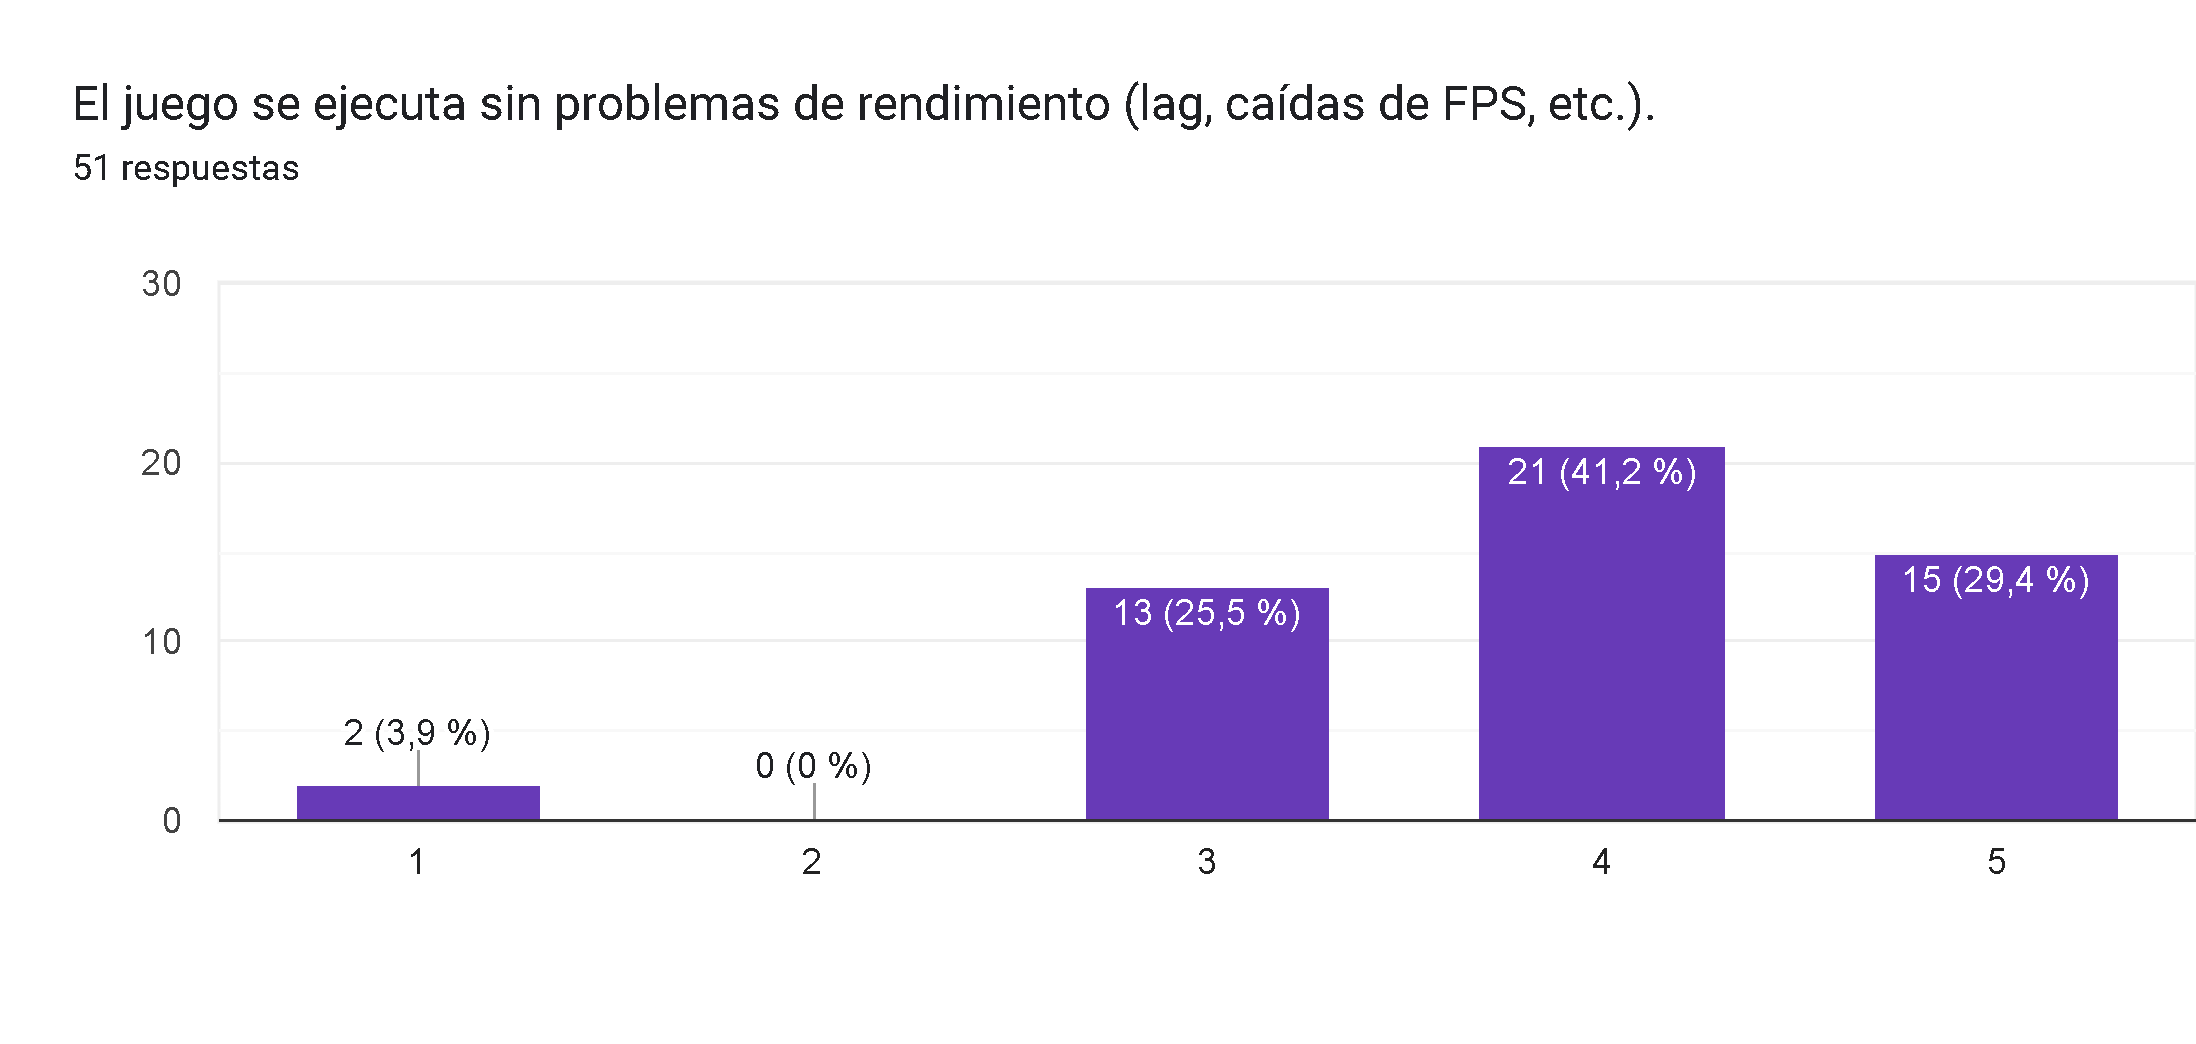
\includegraphics[width=0.7\linewidth]{Imagenes/fd8.png}
  \caption{Elaboración propia, Módulo fitness, Imagen de referencia sobre cuestionario de gamificación para el módulo fitness del juego sobre el movimiento de la espalda, ``El juego se ejecuta sin problemas de rendimiento (lag, caídas de FPS, etc.)``}
  \label{fig:cuestionario19fitness}
\end{figure}

La pregunta ``No he experimentado fallos técnicos o bugs importantes`` obtuvo la mayor cantidad de respuestas en la opción 4, con un 43,1 \%. Además, un 19,6 \% eligió la opción 3, lo que sugiere que la mayoría de los usuarios no han experimentado fallos importantes, aunque un porcentaje significativo aún podría haber encontrado errores menores o bugs en el juego.

\begin{figure}[H]
  \centering
  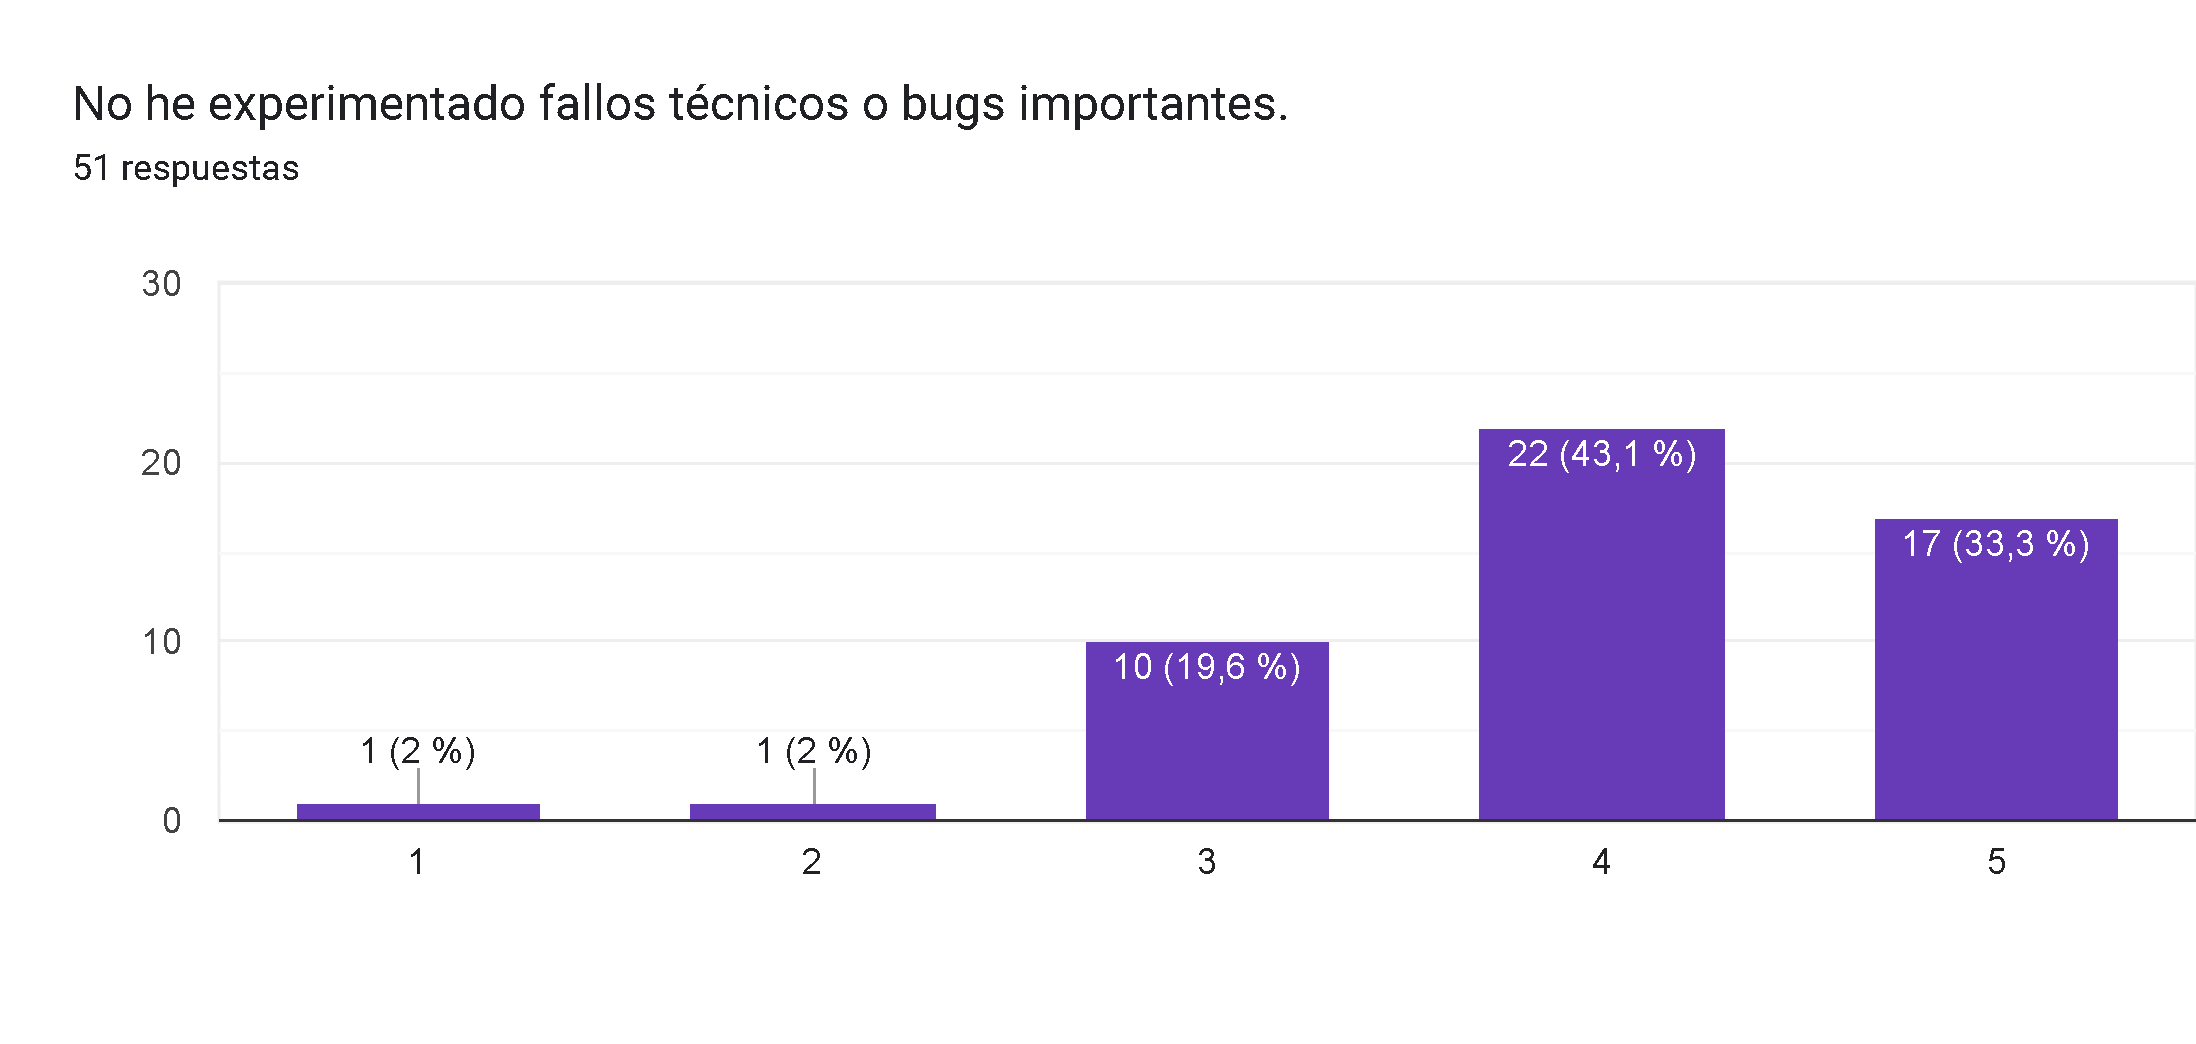
\includegraphics[width=0.7\linewidth]{Imagenes/fd9.png}
  \caption{Elaboración propia, Módulo fitness, Imagen de referencia sobre cuestionario de gamificación para el módulo fitness del juego sobre el movimiento de la espalda, ``No he experimentado fallos técnicos o bugs importantes``}
  \label{fig:cuestionario20fitness}
\end{figure}


La pregunta ``El juego me ha mantenido motivado para seguir jugando`` obtuvo la mayor cantidad de respuestas en la opción 4, con un 41,7 \%. Además, un 31,3 \% de los usuarios eligieron la opción 3, lo que indica que la mayoría se siente motivada para continuar jugando, aunque algunos aún podrían necesitar más incentivos.

\begin{figure}[H]
  \centering
  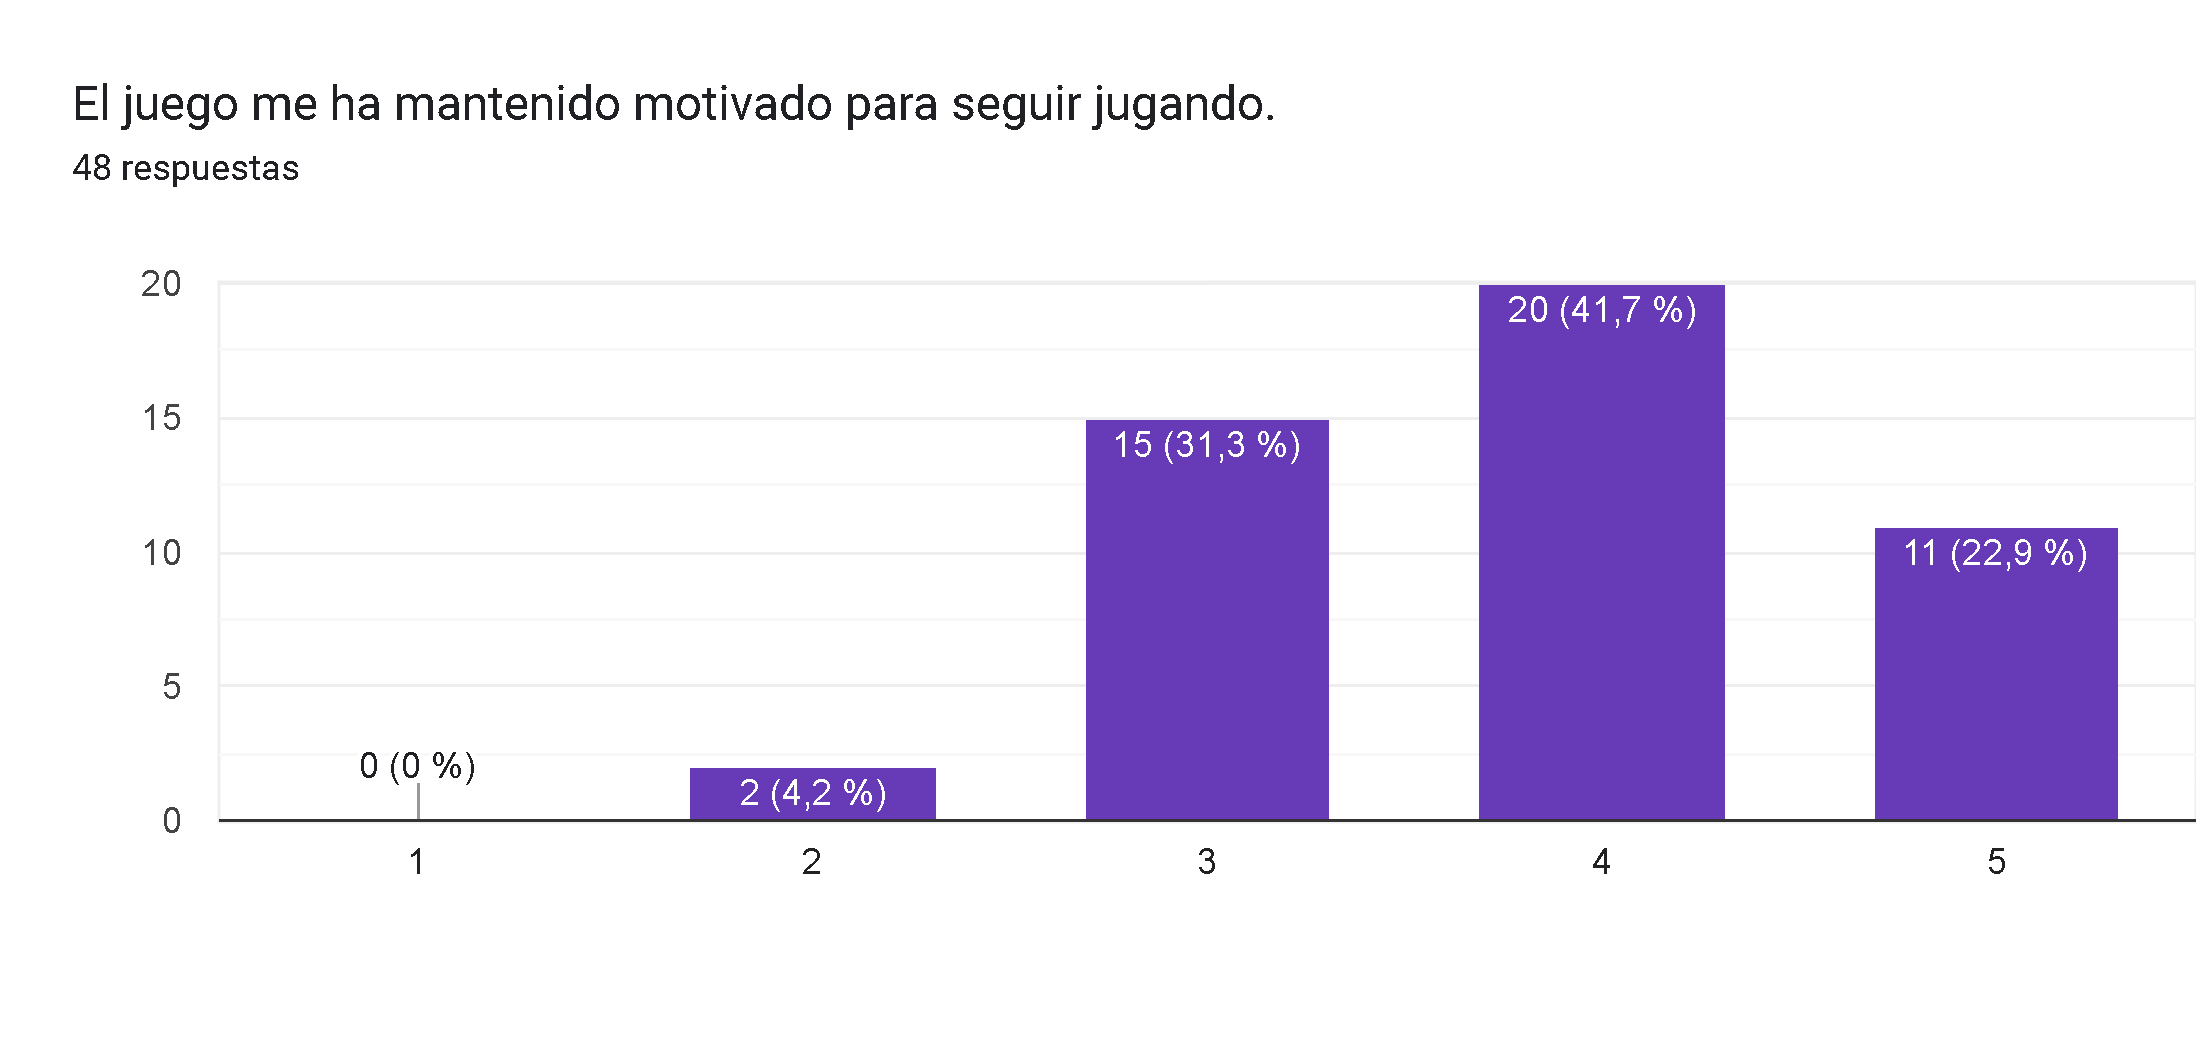
\includegraphics[width=0.7\linewidth]{Imagenes/fd10.png}
  \caption{Elaboración propia, Módulo fitness, Imagen de referencia sobre cuestionario de gamificación para el módulo fitness del juego sobre el movimiento de la espalda, ``El juego me ha mantenido motivado para seguir jugando``}
  \label{fig:cuestionario21fitness}
\end{figure}

La pregunta ``Consideras que el juego es útil para ayudar a la prevención de dolores articulares basados en la espalda`` obtuvo la mayor cantidad de respuestas en la opción 4, con un 47,1 \%, seguida de un 39,2 \% en la opción 5. Esto indica que una mayoría de los usuarios considera que el juego puede ser útil para la prevención de dolores articulares en la espalda, aunque un porcentaje significativo aún tiene dudas al respecto.

\begin{figure}[H]
  \centering
  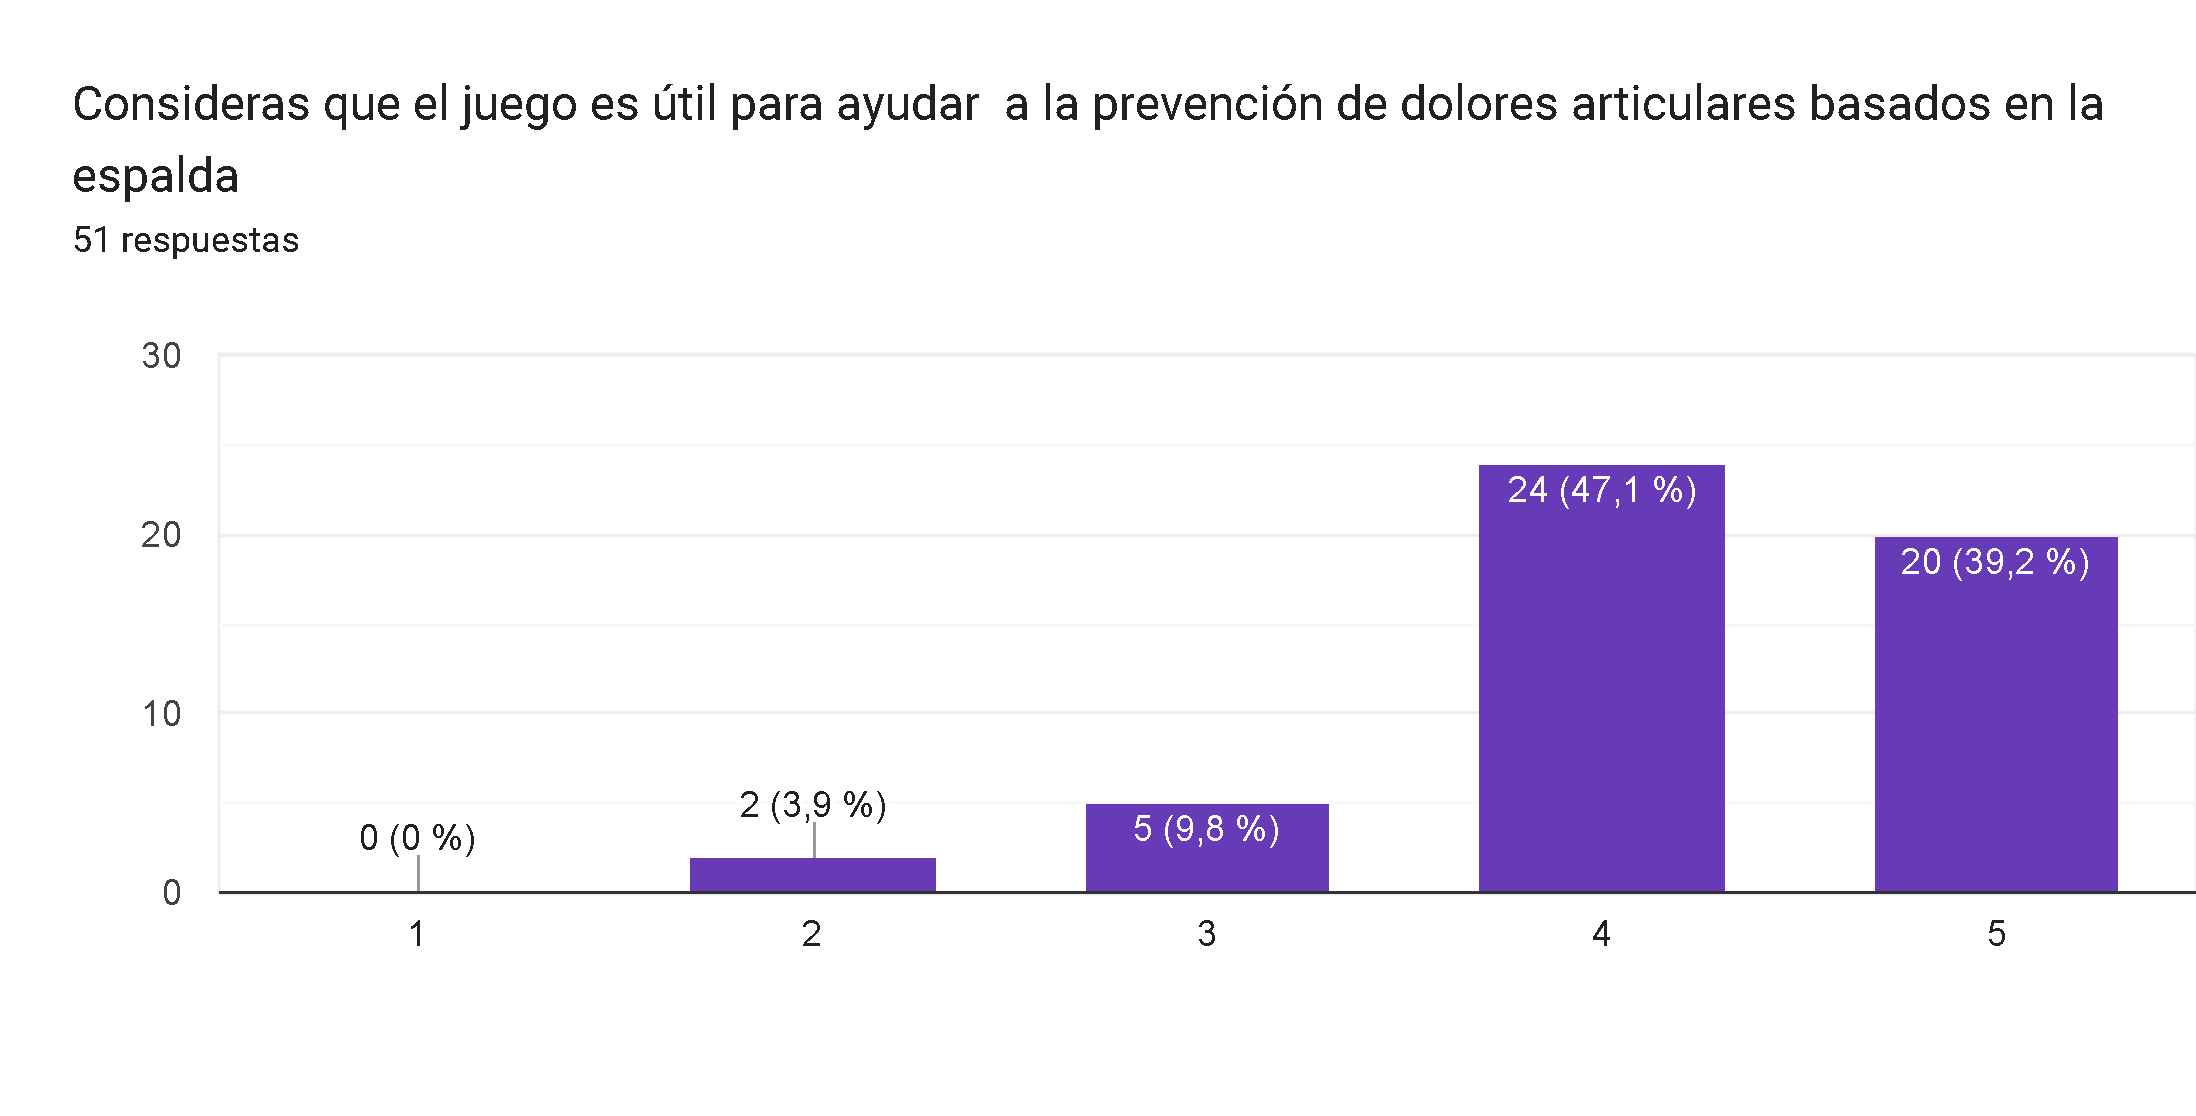
\includegraphics[width=0.7\linewidth]{Imagenes/fd11.png}
  \caption{Elaboración propia, Módulo fitness, Imagen de referencia sobre cuestionario de gamificación para el módulo fitness del juego sobre el movimiento de la espalda, ``Consideras que el juego es útil para ayudar a la prevención de dolores articulares basados en la espalda``}
  \label{fig:cuestionario22fitness}
\end{figure}


La pregunta ``Me siento satisfecho con la experiencia general del juego`` obtuvo la mayor cantidad de respuestas en la opción 4, con un 49 \%, seguida de un 25,5 \% en la opción 5, y de un 21,6 \% en la opción 3. Esto sugiere que la mayoría de los usuarios están satisfechos con la experiencia general del juego, aunque un porcentaje considerable podría tener áreas de mejora o expectativas aún no completamente satisfechas.

\begin{figure}[H]
  \centering
  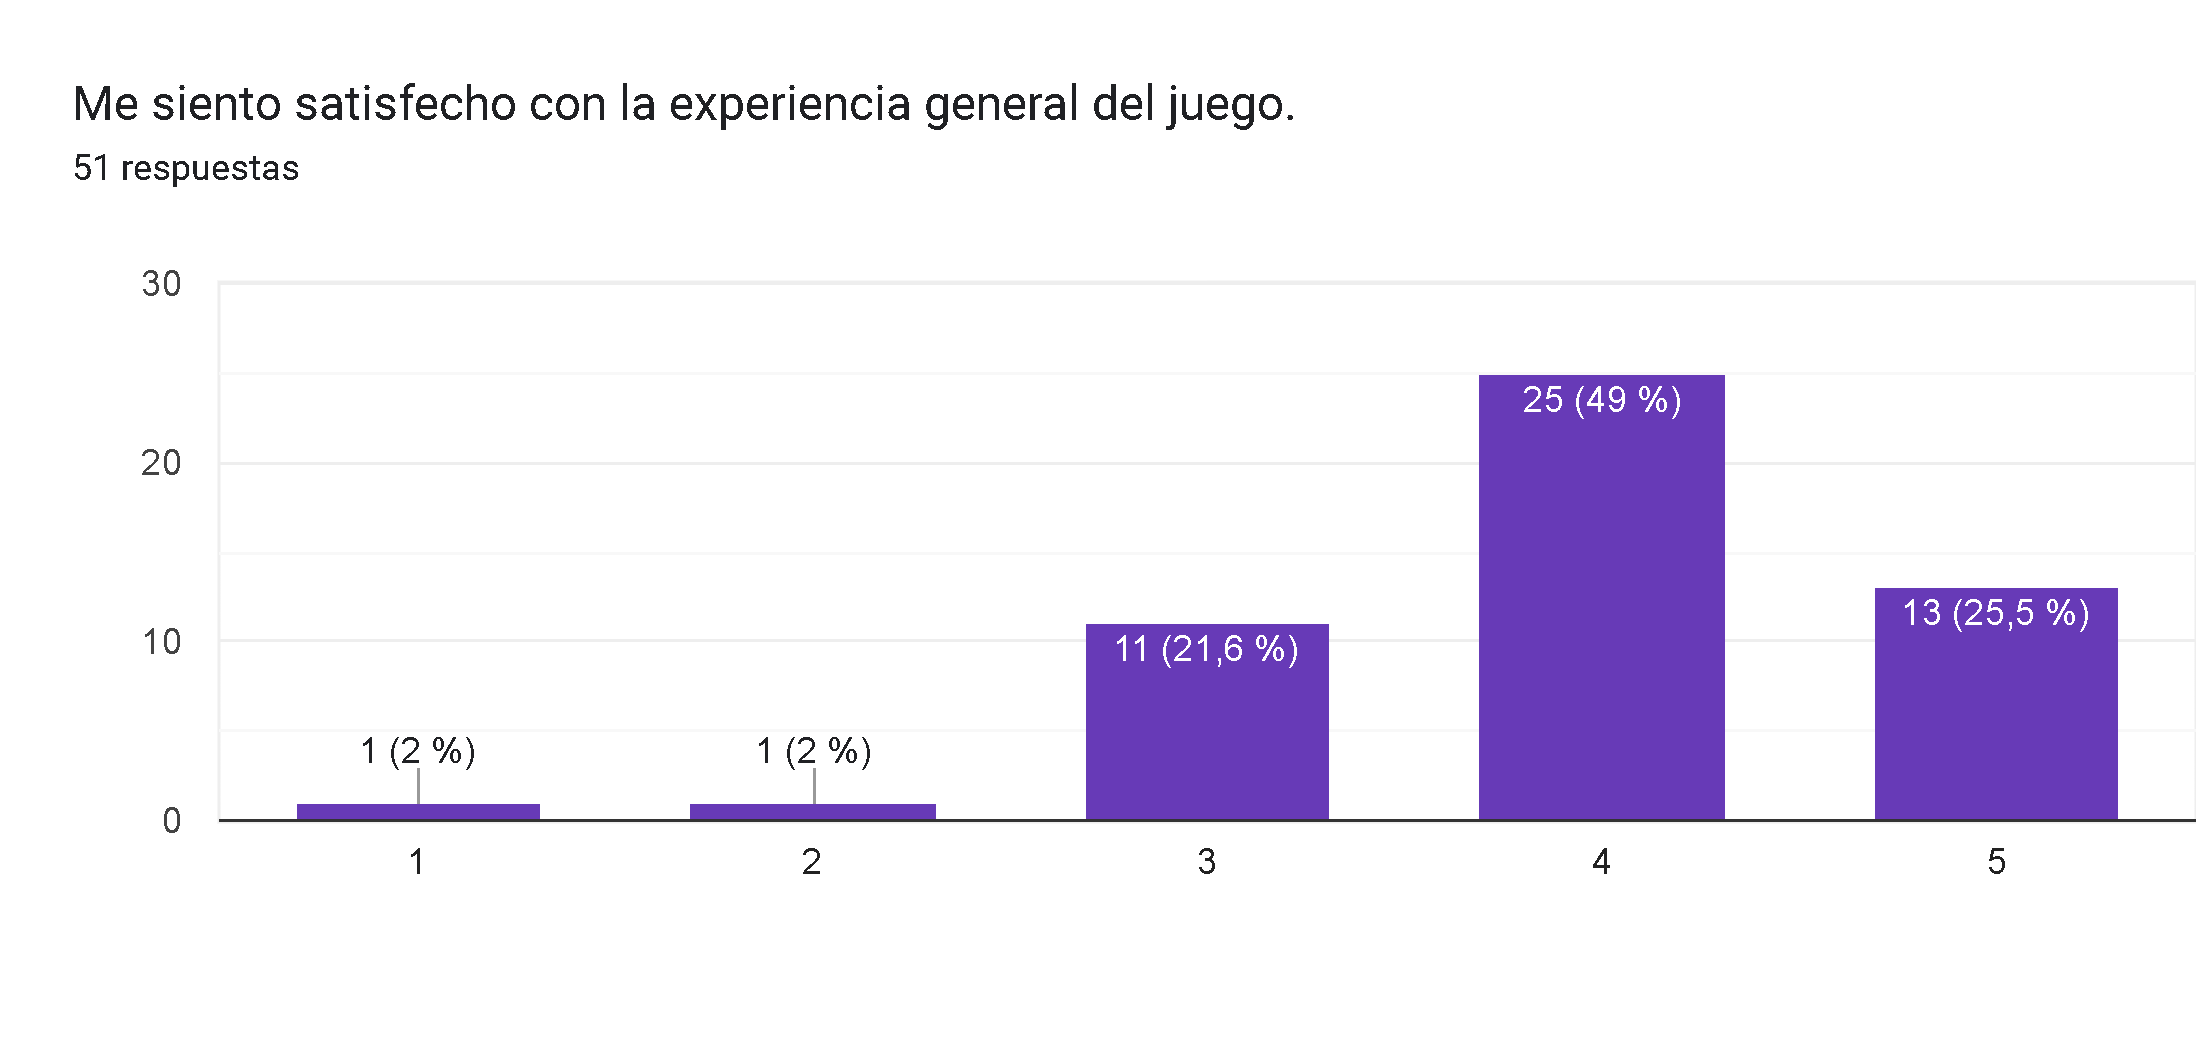
\includegraphics[width=0.7\linewidth]{Imagenes/fd12.png}
  \caption{Elaboración propia, Módulo fitness, Imagen de referencia sobre cuestionario de gamificación para el módulo fitness del juego sobre el movimiento de la espalda, ``Me siento satisfecho con la experiencia general del juego``}
  \label{fig:cuestionario23fitness}
\end{figure}




\subsection{Mindset: Juego sobre puzzles}

La pregunta ``El juego es fácil de entender y aprender`` obtuvo la mayor cantidad de respuestas en la opción 5, con un 41,2 \%. Esto indica que la mayoría de los usuarios consideran que el juego es comprensible y fácil de aprender, aunque una parte también encuentra áreas que podrían mejorarse para facilitar aún más su comprensión.

\begin{figure}[H]
  \centering
  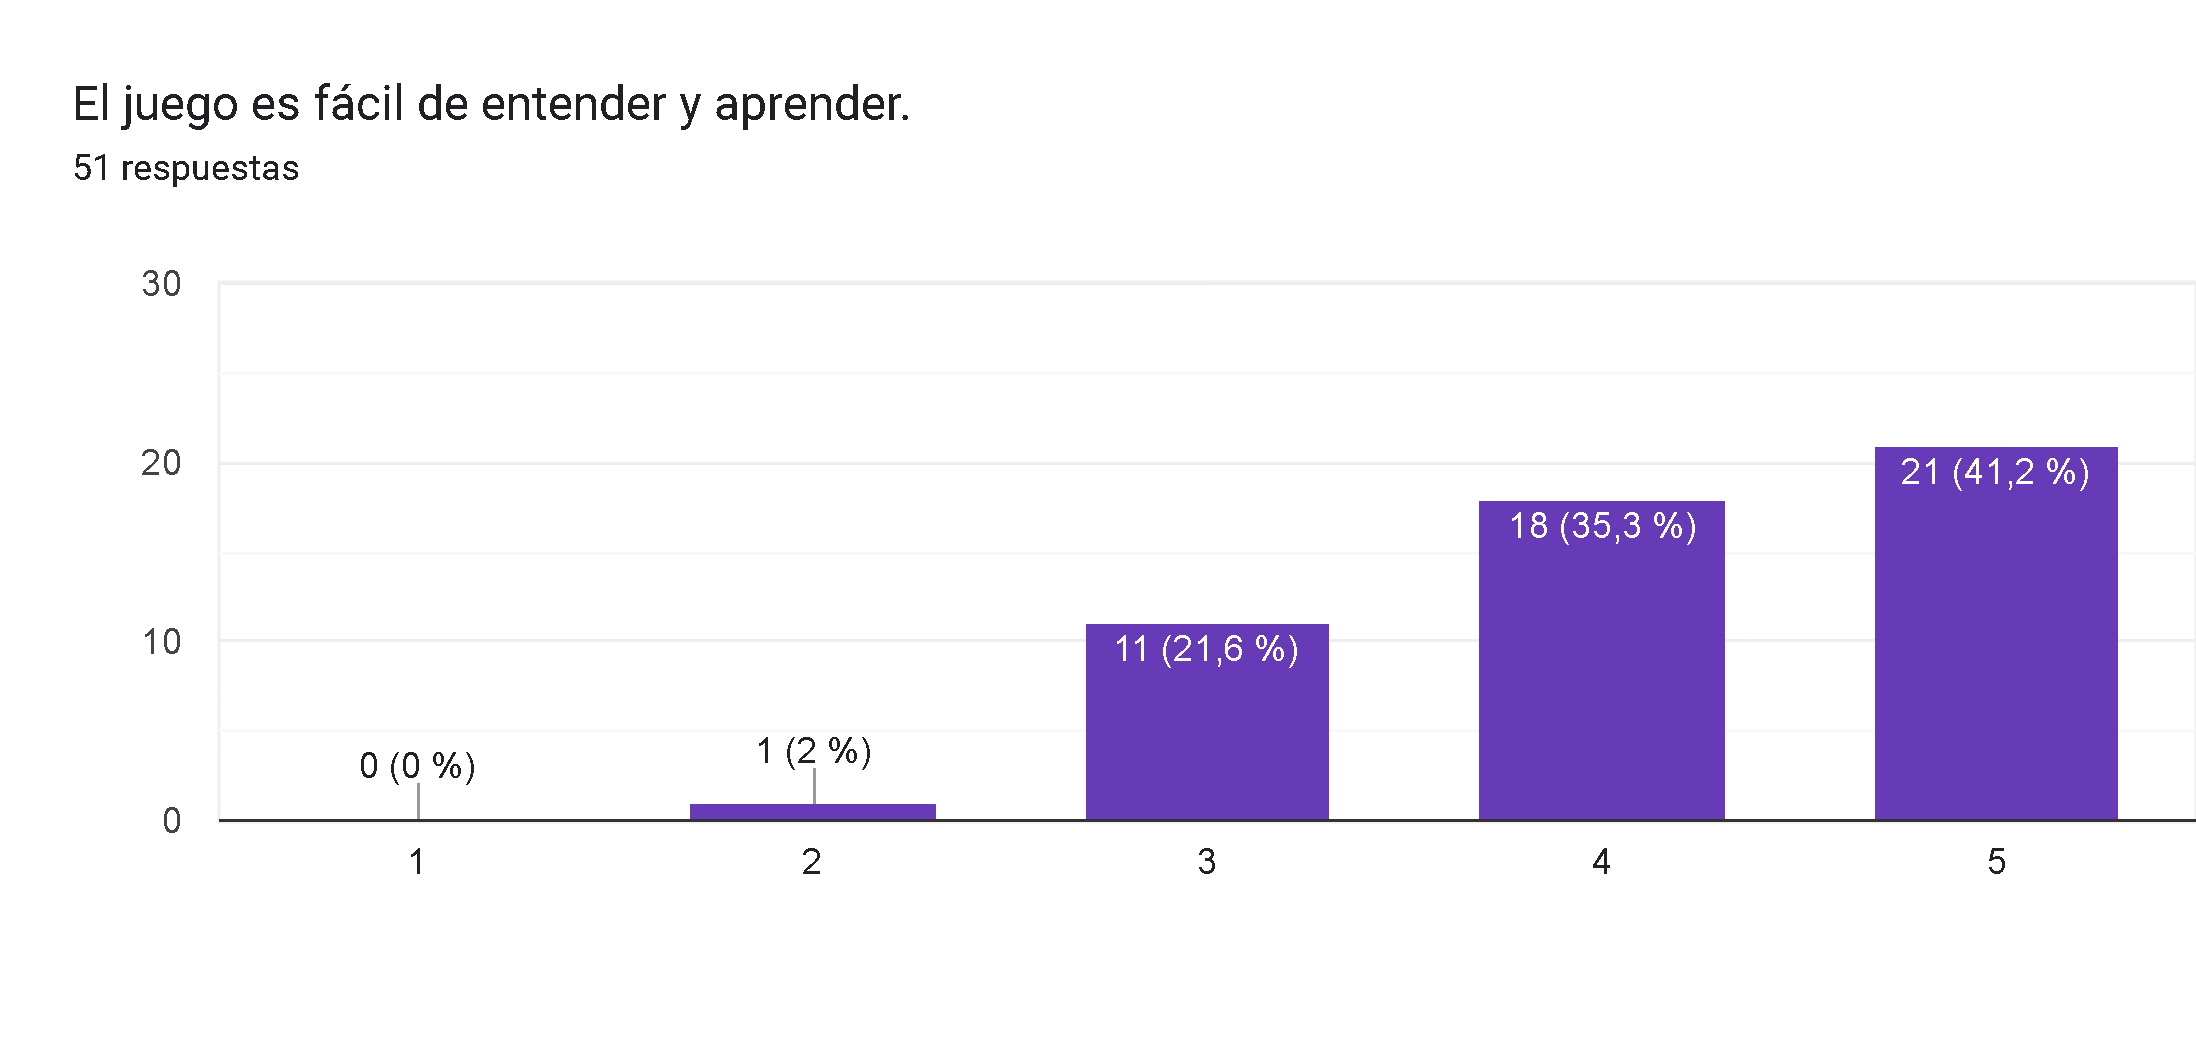
\includegraphics[width=0.7\linewidth]{Imagenes/mc1.png}
  \caption{Elaboración propia, Módulo mindset, Imagen de referencia sobre cuestionario de gamificación para el módulo mindset del juego sobre puzzles, ``El juego es fácil de entender y aprender``}
  \label{fig:cuestionario1mindset}
\end{figure}



La pregunta ``Los controles son intuitivos y responden bien`` obtuvo la mayor cantidad de respuestas en la opción 5, con un 39,2 \%. Esto sugiere que la mayoría de los usuarios consideran que los controles responden de manera adecuada y son fáciles de entender, mientras que un porcentaje considerable también seleccionó la opción 4, con un 37,3 \%, indicando una evaluación positiva pero con espacio para mejoras.

\begin{figure}[H]
  \centering
  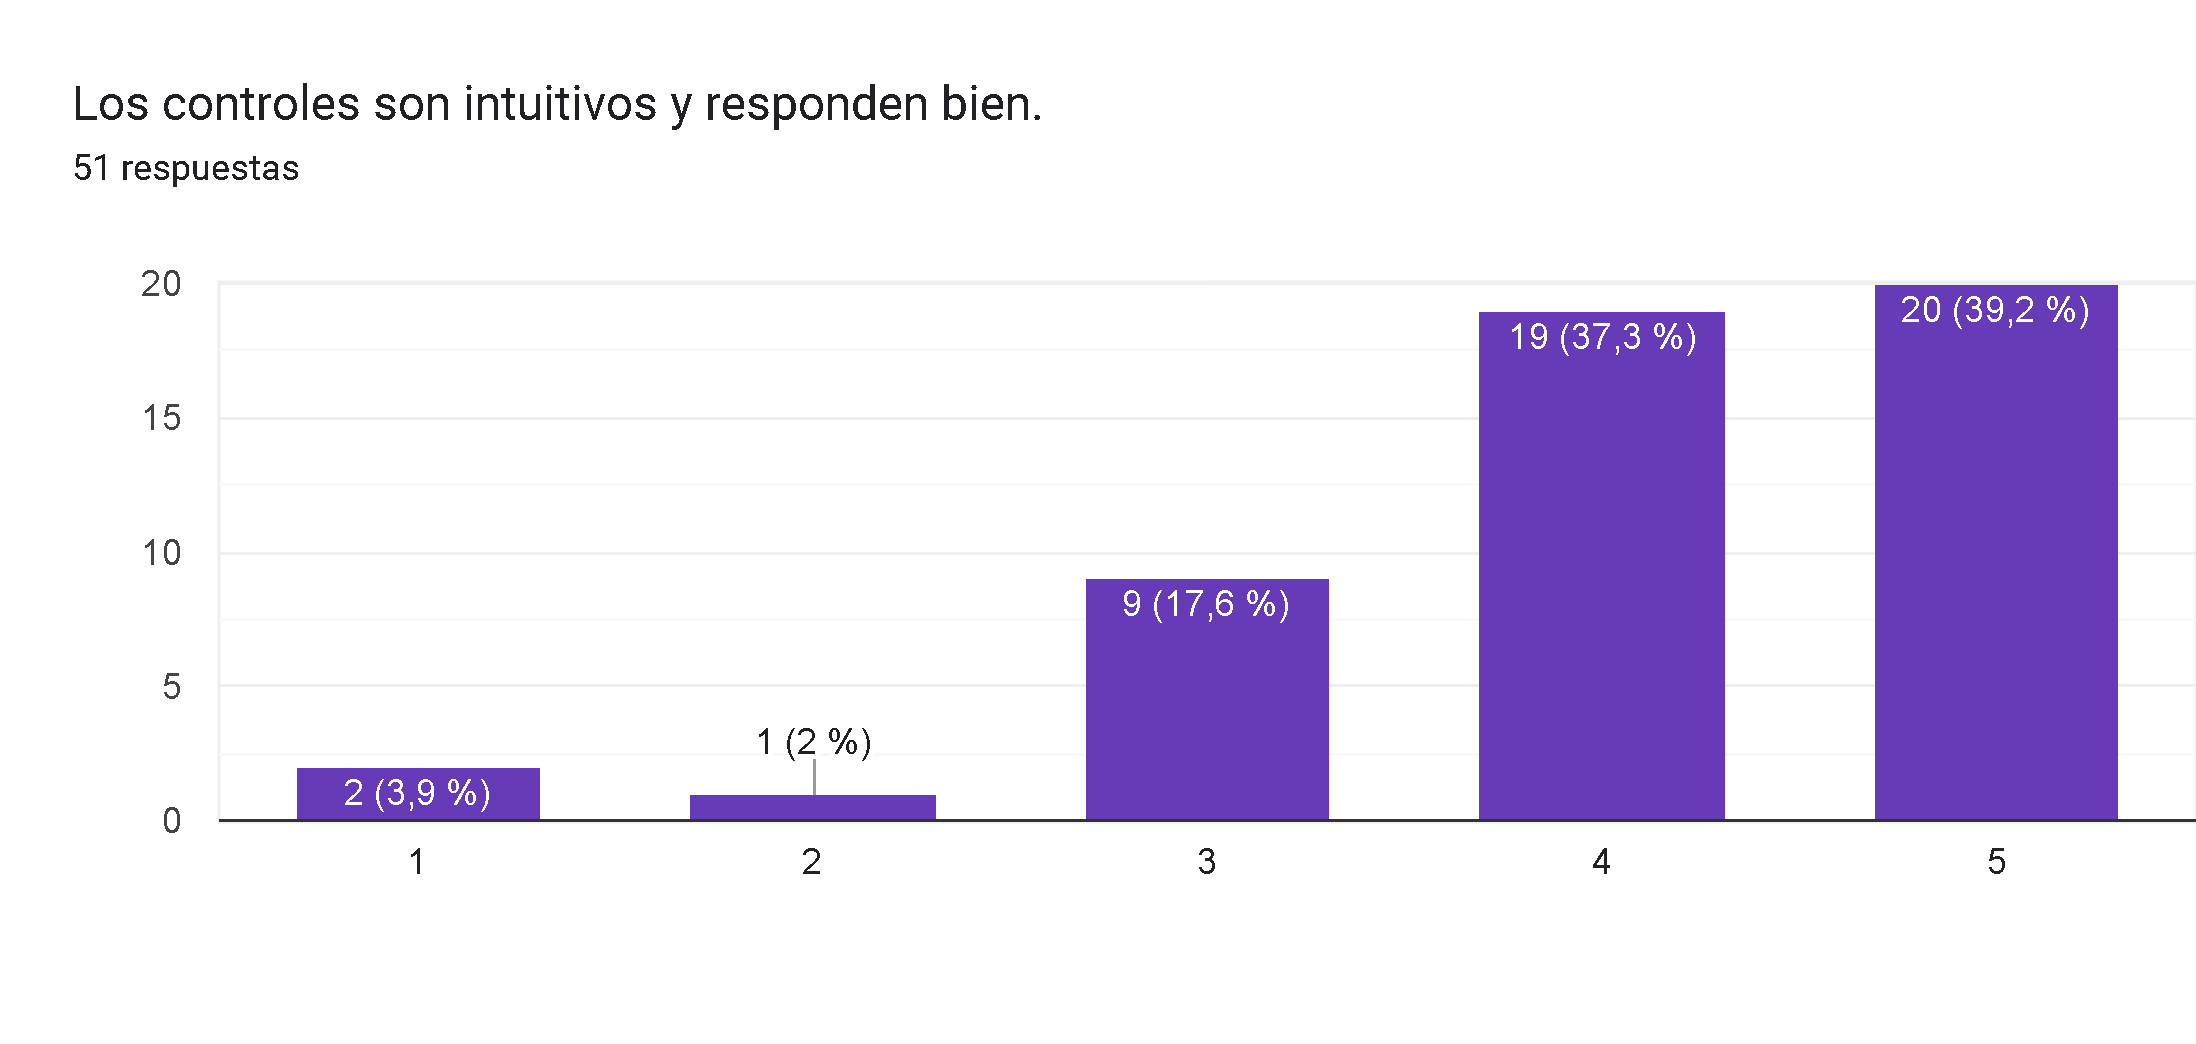
\includegraphics[width=0.7\linewidth]{Imagenes/mc2.png}
  \caption{Elaboración propia, Módulo mindset, Imagen de referencia sobre cuestionario de gamificación para el módulo mindset del juego sobre puzzles, ``Los controles son intuitivos y responden bien``}
  \label{fig:cuestionario2mindset}
\end{figure}

La pregunta ``El nivel de dificultad es adecuado`` obtuvo la mayor cantidad de respuestas en la opción 4, con un 47,1 \%. Esto sugiere que la mayoría de los usuarios consideran que el nivel de dificultad está bien equilibrado, proporcionando una experiencia desafiante pero no excesivamente difícil para la mayoría de los jugadores.

\begin{figure}[H]
  \centering
  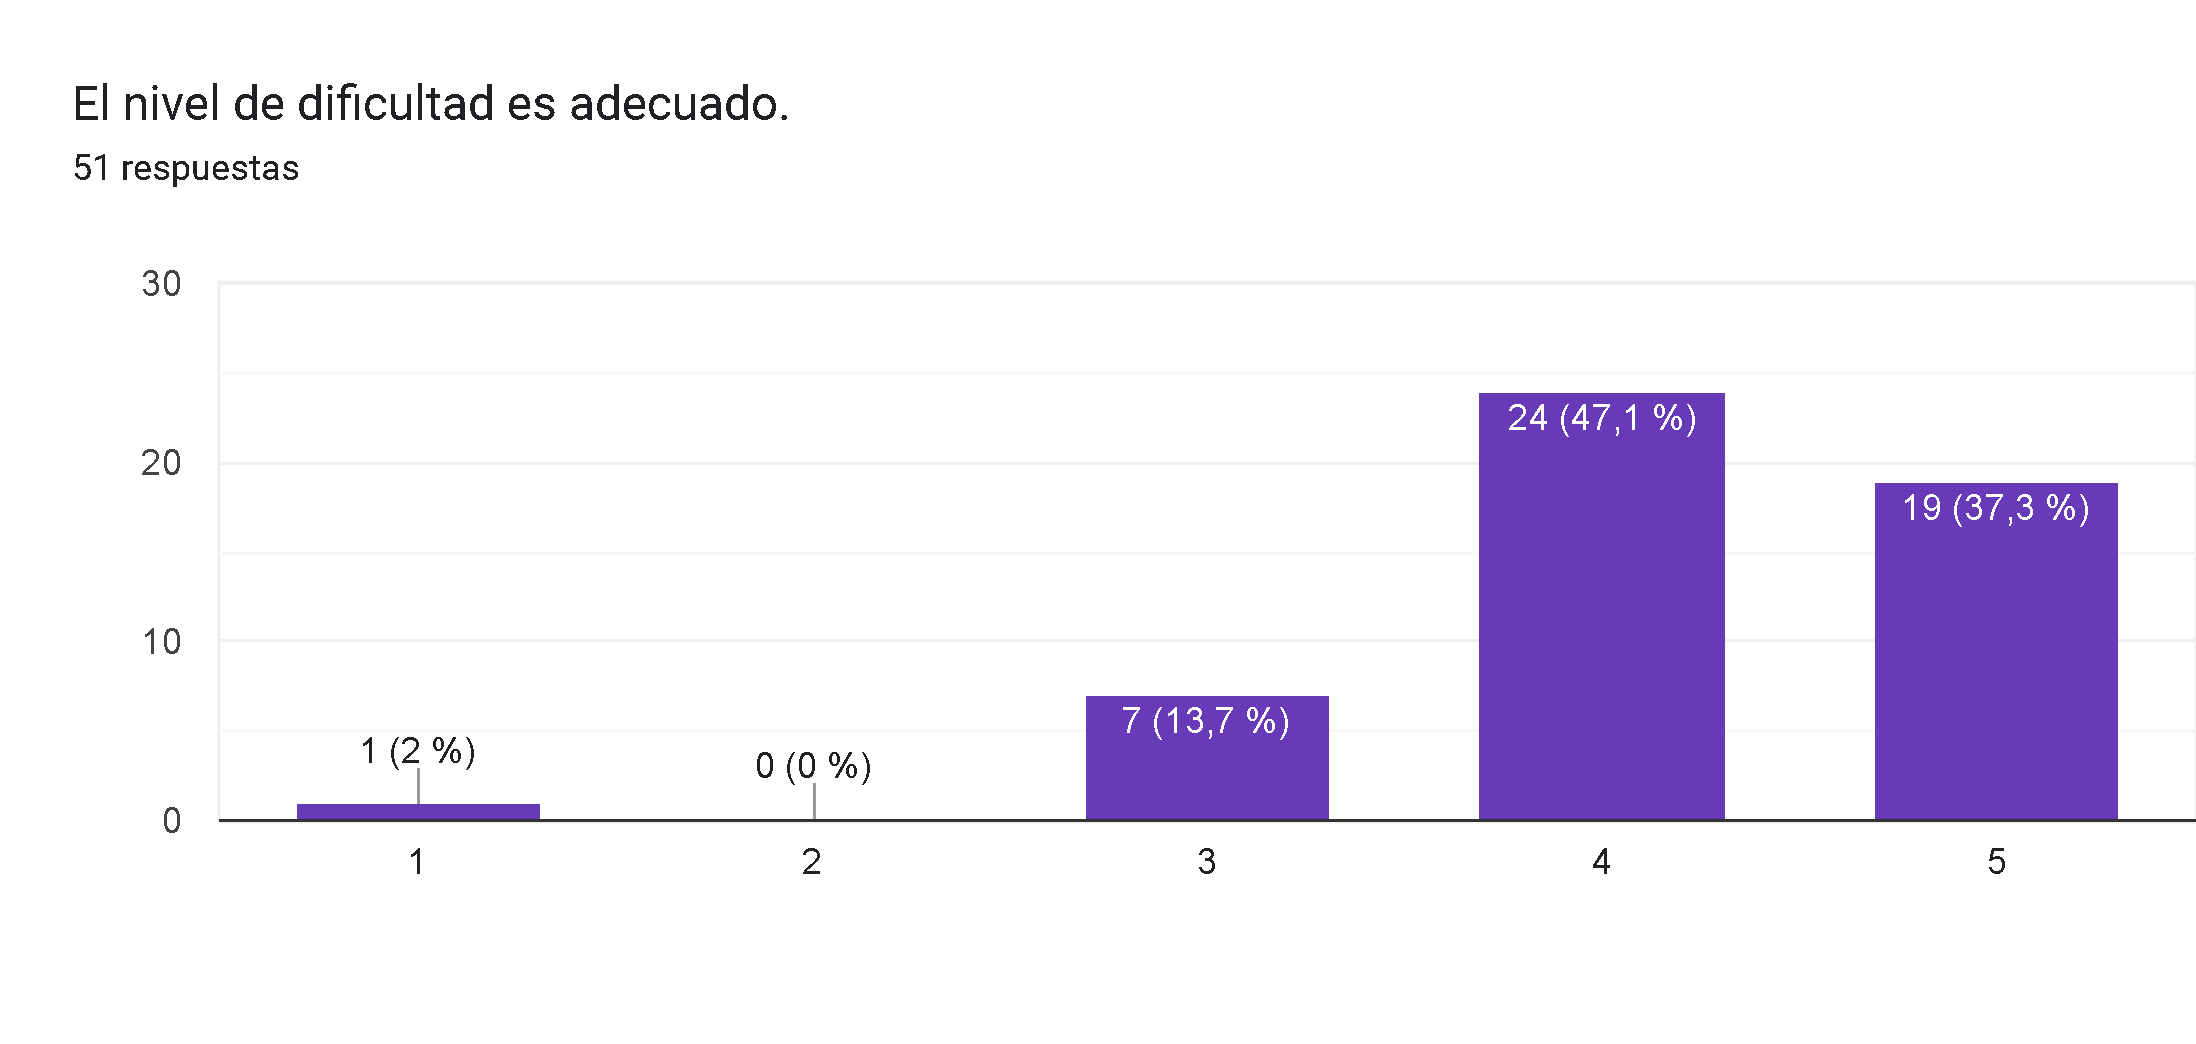
\includegraphics[width=0.7\linewidth]{Imagenes/mc3.png}
  \caption{Elaboración propia, Módulo mindset, Imagen de referencia sobre cuestionario de gamificación para el módulo mindset del juego sobre puzzles, ``El nivel de dificultad es adecuado``}
  \label{fig:cuestionario3mindset}
\end{figure}



La pregunta ``La interfaz del usuario es clara y fácil de usar`` obtuvo la mayor cantidad de respuestas en la opción 4, seguida de la opción 5. Esto indica que la mayoría de los usuarios encuentran la interfaz clara y fácil de usar, aunque un porcentaje también considera que podría haber áreas de mejora en su accesibilidad o claridad.

\begin{figure}[H]
  \centering
  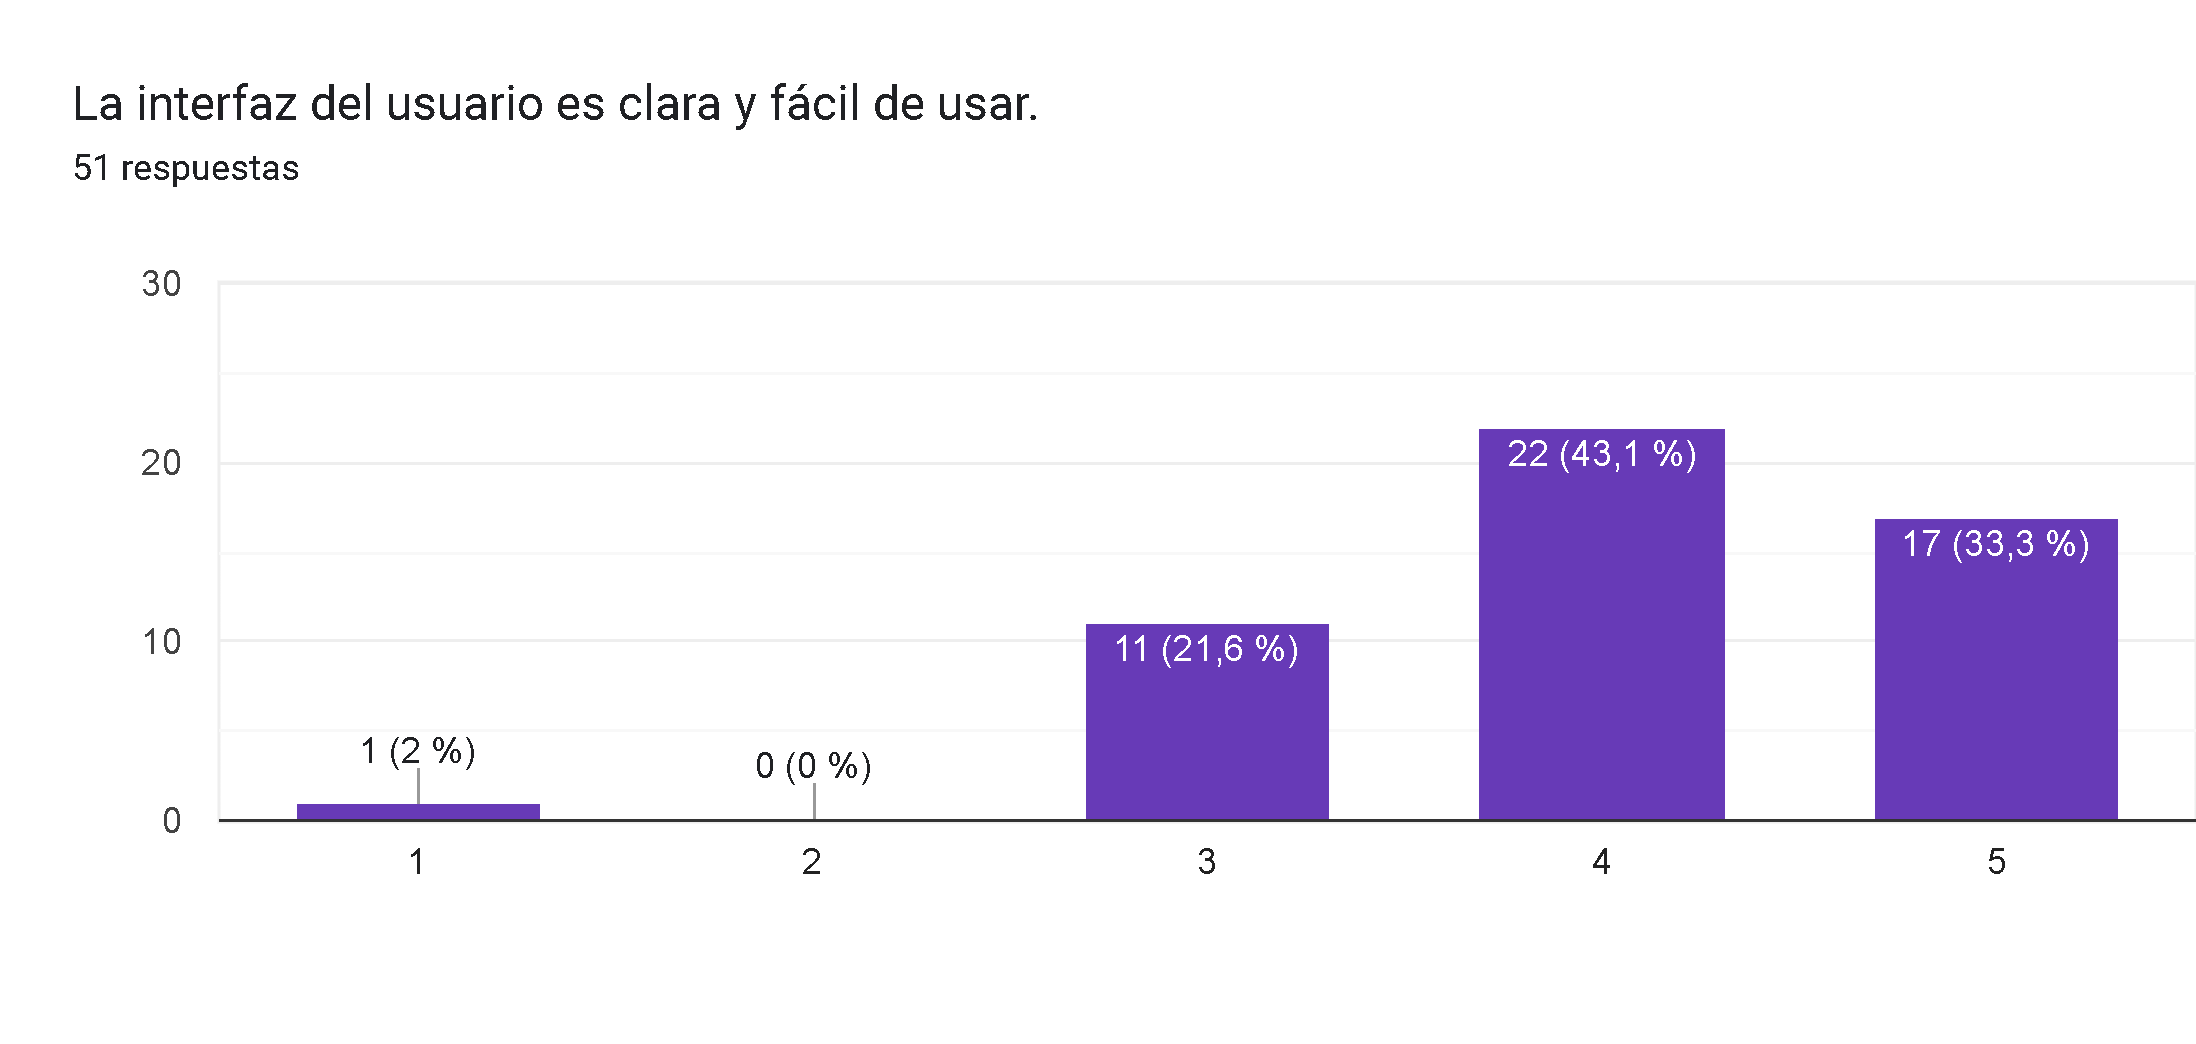
\includegraphics[width=0.7\linewidth]{Imagenes/mc4.png}
  \caption{Elaboración propia, Módulo mindset, Imagen de referencia sobre cuestionario de gamificación para el módulo mindset del juego sobre puzzles, ``La interfaz del usuario es clara y fácil de usar``}
  \label{fig:cuestionario4mindset}
\end{figure}

La pregunta ``La música del juego es adecuada y mejora la experiencia`` obtuvo la mayor cantidad de respuestas en la opción 4, con un 39,2 \%. La opción 3 recibió un 19,6 \%, mientras que un 35,3 \% optó por la opción 5. Esto sugiere que la mayoría de los usuarios considera que la música contribuye positivamente a la experiencia, aunque aún hay algunos que tienen dudas al respecto o consideran que puede mejorarse.

\begin{figure}[H]
  \centering
  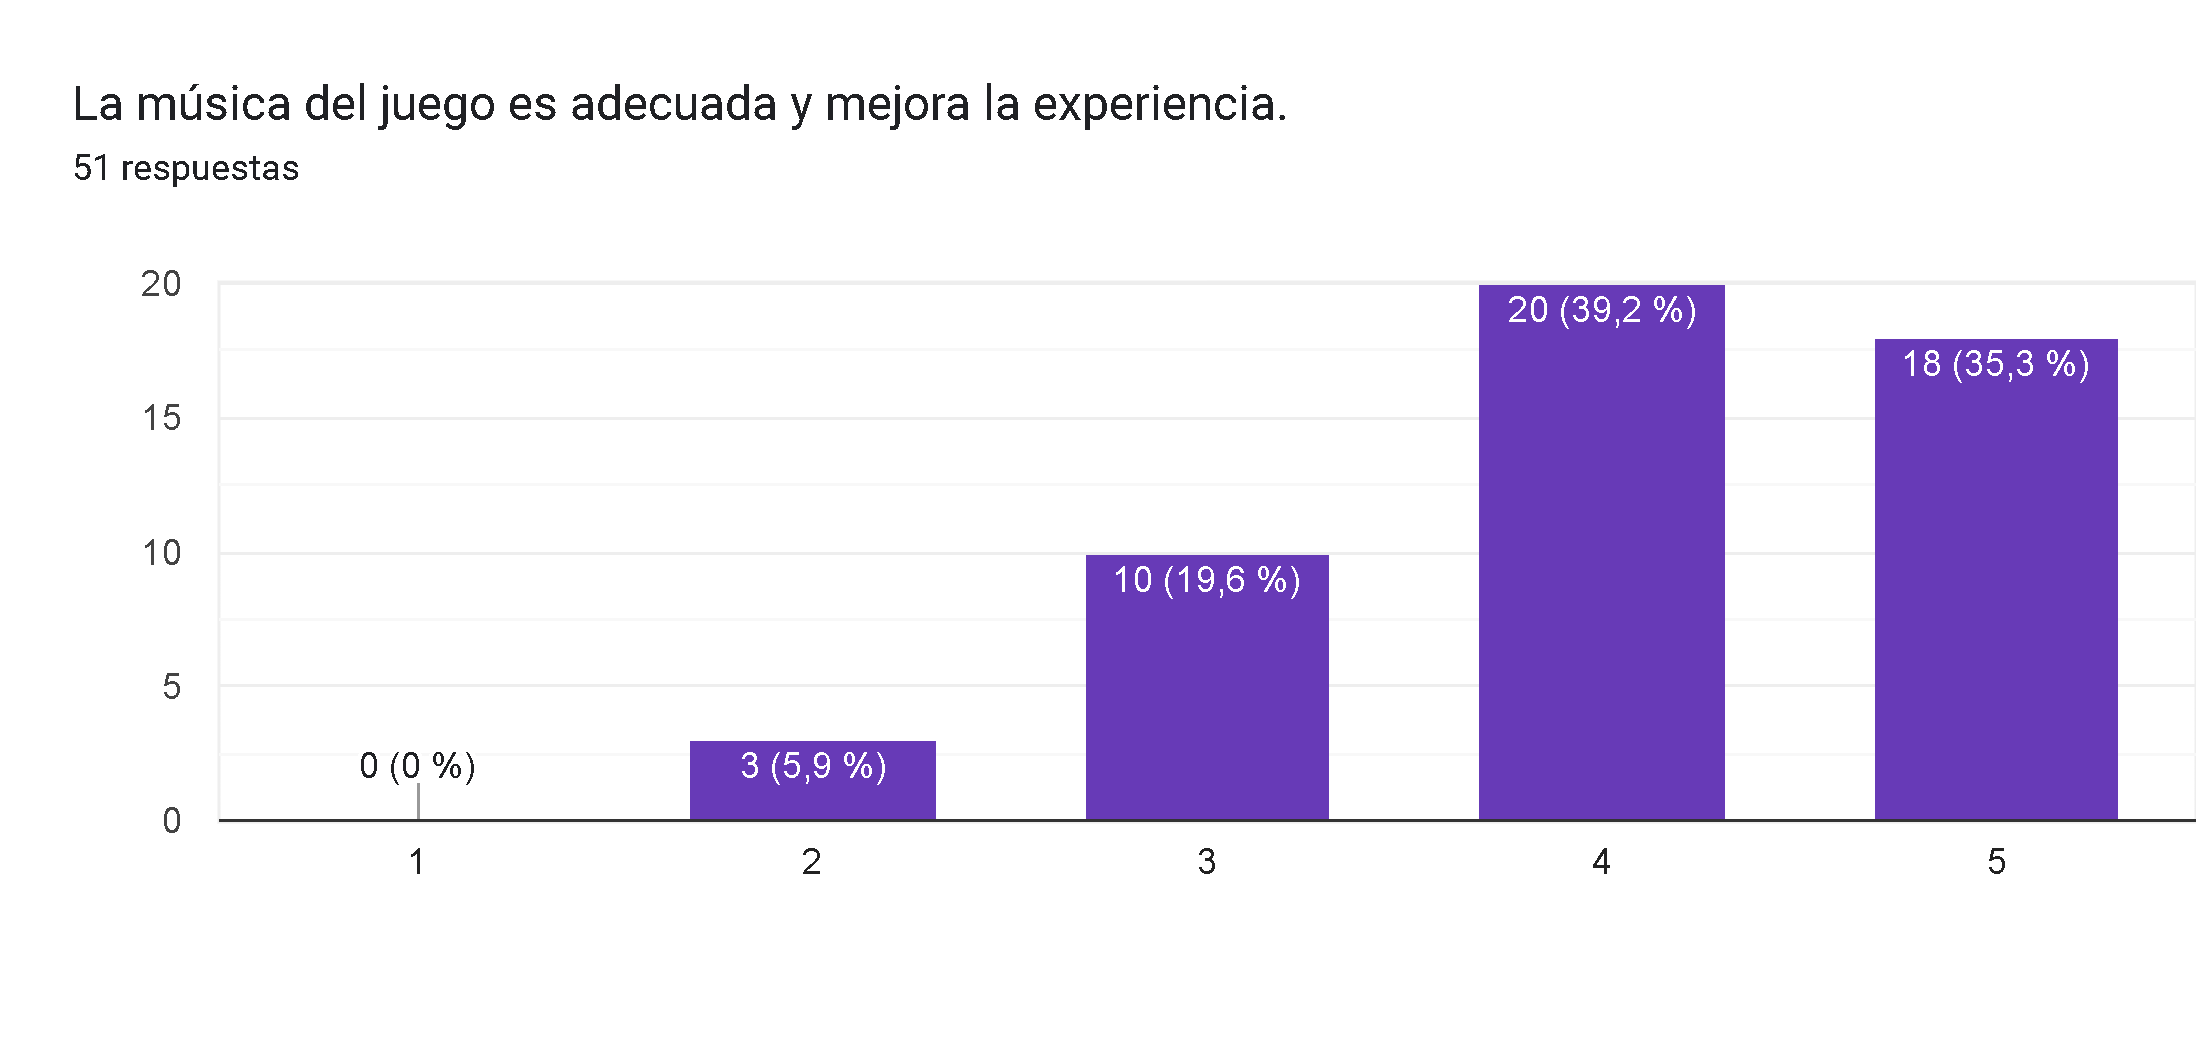
\includegraphics[width=0.7\linewidth]{Imagenes/mc5.png}
  \caption{Elaboración propia, Módulo mindset, Imagen de referencia sobre cuestionario de gamificación para el módulo mindset del juego sobre puzzles, ``La música del juego es adecuada y mejora la experiencia``}
  \label{fig:cuestionario5mindset}
\end{figure}



La pregunta ``El juego se ejecuta sin problemas de rendimiento (lag, caídas de FPS, etc.)`` obtuvo la mayor cantidad de respuestas en la opción 5, con un 41,2 \%. Esto indica que la mayoría de los usuarios experimenta un rendimiento sin problemas significativos.

\begin{figure}[H]
  \centering
  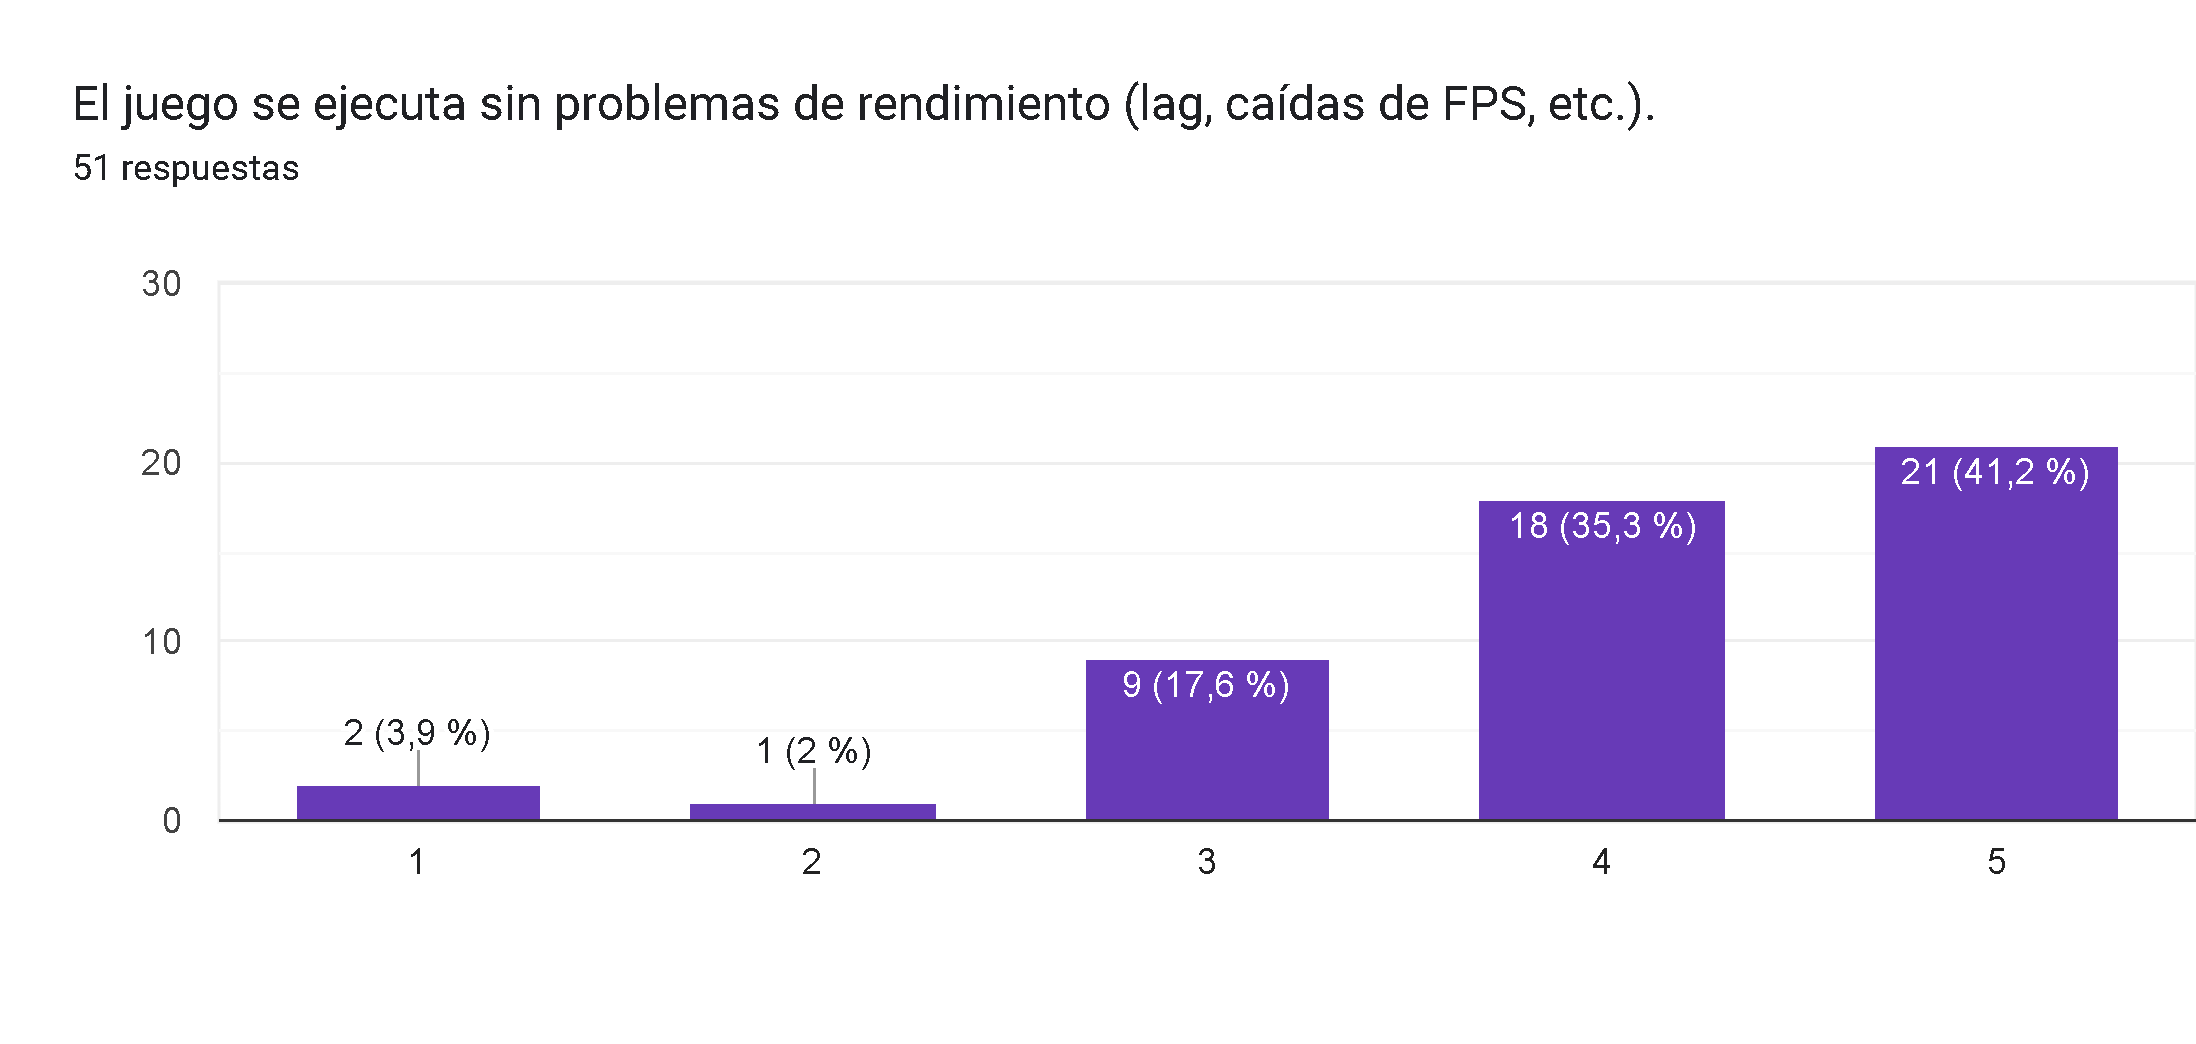
\includegraphics[width=0.7\linewidth]{Imagenes/mc6.png}
  \caption{Elaboración propia, Módulo mindset, Imagen de referencia sobre cuestionario de gamificación para el módulo mindset del juego sobre puzzles, ``El juego se ejecuta sin problemas de rendimiento (lag, caídas de FPS, etc.)``}
  \label{fig:cuestionario6mindset}
\end{figure}

La pregunta ``No he experimentado fallos técnicos o bugs importantes`` obtuvo la mayor cantidad de respuestas en la opción 4, con 25 respuestas. Esto sugiere que la mayoría de los usuarios no han experimentado fallos importantes, aunque aún hay algunos que podrían haber encontrado errores menores o bugs en el juego.

\begin{figure}[H]
  \centering
  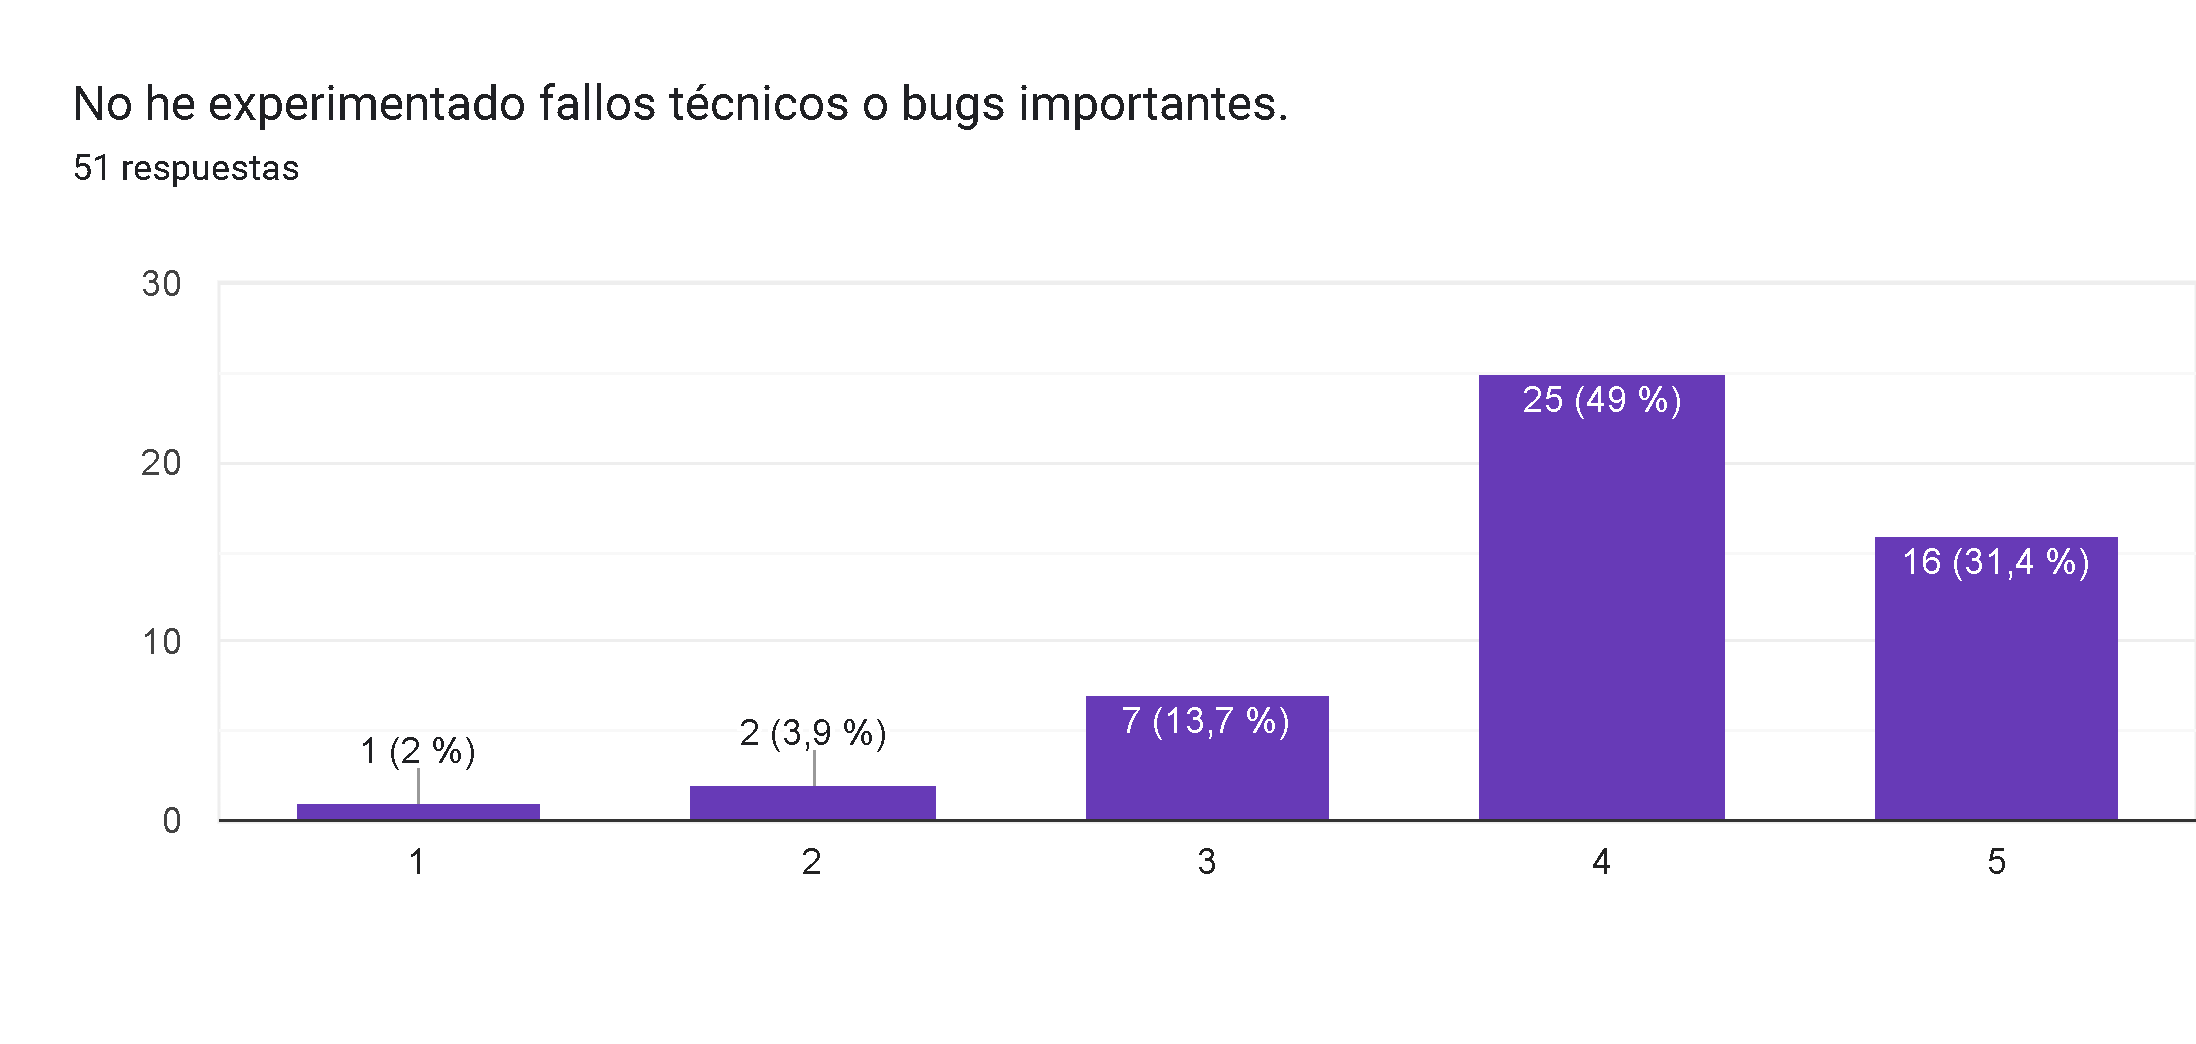
\includegraphics[width=0.7\linewidth]{Imagenes/mc7.png}
  \caption{Elaboración propia, Módulo mindset, Imagen de referencia sobre cuestionario de gamificación para el módulo mindset del juego sobre puzzles, ``No he experimentado fallos técnicos o bugs importantes``}
  \label{fig:cuestionario7mindset}
\end{figure}



La pregunta ``El juego me ha mantenido motivado para seguir jugando`` obtuvo la mayor cantidad de respuestas en la opción 5, con un 42 \%. Esto indica que la mayoría de los usuarios se sienten motivados para continuar jugando, aunque un porcentaje también respondió afirmativamente en la opción 4, con un 32 \%.

\begin{figure}[H]
  \centering
  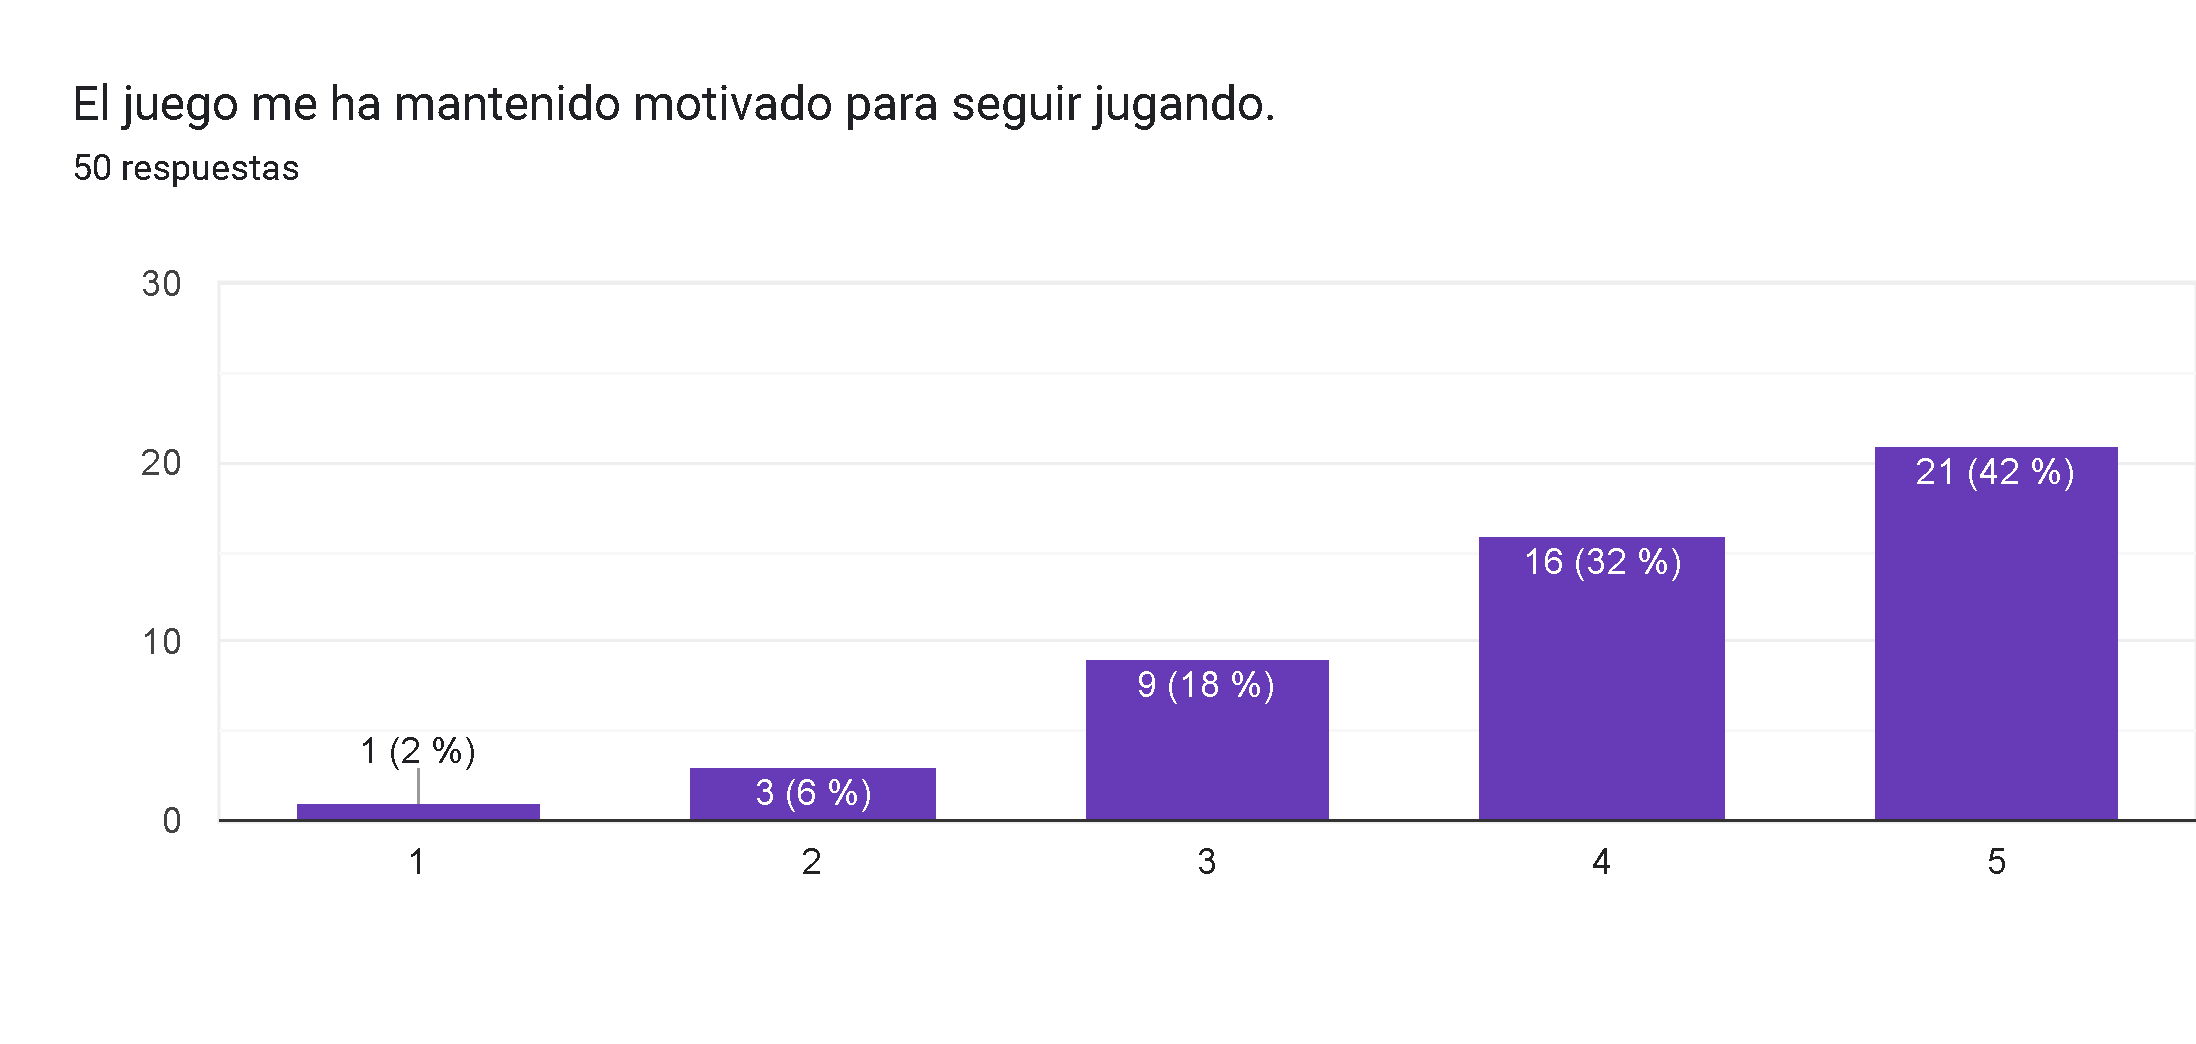
\includegraphics[width=0.7\linewidth]{Imagenes/mc8.png}
  \caption{Elaboración propia, Módulo mindset, Imagen de referencia sobre cuestionario de gamificación para el módulo mindset del juego sobre puzzles, ``El juego me ha mantenido motivado para seguir jugando``}
  \label{fig:cuestionario8mindset}
\end{figure}



La pregunta ``Me siento satisfecho con la experiencia general del juego`` obtuvo la mayor cantidad de respuestas en la opción 4, con un 42,9 \%. Esto indica que la mayoría de los usuarios están satisfechos con la experiencia general del juego, mientras que un porcentaje significativo también eligió la opción 5, con un 38,8 \%.

\begin{figure}[H]
  \centering
  \includegraphics[width=0.7\linewidth]{Imagenes/mc9.png}
  \caption{Elaboración propia, Módulo mindset, Imagen de referencia sobre cuestionario de gamificación para el módulo mindset del juego sobre puzzles, ``Me siento satisfecho con la experiencia general del juego``}
  \label{fig:cuestionario9mindset}
\end{figure}



La pregunta ``Consideras que el juego es útil para el desarrollo de habilidades deductivas`` obtuvo la mayor cantidad de respuestas en la opción 5, con un 43,1 \%. Además, un 37,3 \% eligió la opción 4, lo que sugiere que una mayoría considera que el juego es útil para desarrollar habilidades deductivas, aunque también hay una proporción significativa que tiene una opinión positiva, pero no tan rotunda.

\begin{figure}[H]
  \centering
  \includegraphics[width=0.7\linewidth]{Imagenes/mc10.png}
  \caption{Elaboración propia, Módulo mindset, Imagen de referencia sobre cuestionario de gamificación para el módulo mindset del juego sobre puzzles, ``Consideras que el juego es útil para el desarrollo de habilidades deductivas``}
  \label{fig:cuestionario10mindset}
\end{figure}

La pregunta ``Consideras que el juego es útil para el desarrollo de la resiliencia y el cómo afrontar los desafíos`` obtuvo la mayor cantidad de respuestas en la opción 4, con un 50 \%. Esto indica que la mayoría de los usuarios considera que el juego tiene un impacto positivo en el desarrollo de la resiliencia y la capacidad para afrontar los desafíos.

\begin{figure}[H]
  \centering
  \includegraphics[width=0.7\linewidth]{Imagenes/mc11.png}
  \caption{Elaboración propia, Módulo mindset, Imagen de referencia sobre cuestionario de gamificación para el módulo mindset del juego sobre puzzles, ``Consideras que el juego es útil para el desarrollo de la resiliencia y el cómo afrontar los desafíos``}
  \label{fig:cuestionario11mindset}
\end{figure}


\section{Cuestionario sobre pruebas de usabilidad heurísticas de Nielsen para plataforma gamificada sobre módulos Mindset y Fitness}
La pregunta ``¿La plataforma te mantuvo informado sobre el progreso del juego o el estado actual, como tiempos de carga o indicadores de avance en los ejercicios de fitness y mindset?'' obtuvo la mayor cantidad de respuestas en la opción 5, con un 50\%. Esto sugiere que la mayoría de los usuarios se sintieron informados sobre su progreso durante el juego, apreciando los indicadores de avance y tiempos de carga. Además, un 30\% de los usuarios seleccionaron la opción 3, lo que indica que una parte también percibió cierta falta de información o detalles sobre el estado del juego. Un 20\% de los usuarios respondió en la opción 2, lo que podría indicar que algunos encontraron insuficiente la información proporcionada por la plataforma.

\begin{figure}[H]
  \centering
  \includegraphics[width=0.7\linewidth]{Imagenes/Nc1.png}
  \caption{Elaboración propia, Imagen de referencia de cuestionario sobre pruebas de usabilidad heurísticas de Nielsen para plataforma gamificada sobre módulos Mindset y Fitness, `¿La plataforma te mantuvo informado sobre el progreso del juego o el estado actual, como tiempos de carga o indicadores de avance en los ejercicios de fitness y mindset?'}

  \label{fig:cuestionario1nielsen}
\end{figure}

La pregunta ``¿Los términos utilizados en los juegos (por ejemplo, instrucciones de ejercicios) fueron fáciles de entender y reflejaron el lenguaje que esperas en estos contextos?'' obtuvo la mayor cantidad de respuestas en la opción 5, con un 50\%. Esto indica que la mayoría de los usuarios encontraron los términos utilizados en el juego claros y apropiados para el contexto. Además, un 30\% de los usuarios seleccionaron la opción 3, lo que sugiere que algunos usuarios consideraron que los términos eran comprensibles, pero podrían mejorarse. Un 20\% de los usuarios eligió la opción 2, lo que podría señalar que algunos encontraron dificultad con el lenguaje utilizado en las instrucciones o el contenido del juego.

\begin{figure}[H]
  \centering
  \includegraphics[width=0.7\linewidth]{Imagenes/Nc2.png}
  \caption{Elaboración propia, Imagen de referencia de cuestionario sobre pruebas de usabilidad heurísticas de Nielsen para plataforma gamificada sobre módulos Mindset y Fitness, `¿Los términos utilizados en los juegos (por ejemplo, instrucciones de ejercicios) fueron fáciles de entender y reflejaron el lenguaje que esperas en estos contextos?'}

  \label{fig:cuestionario2nielsen}
\end{figure}

La pregunta ``¿Pudiste salir o reiniciar los juegos de fitness y mindset fácilmente si cometiste un error o deseabas volver a intentarlo?'' obtuvo la mayor cantidad de respuestas en la opción 5, con un 50\%. Esto indica que la mayoría de los usuarios consideraron que la opción para reiniciar o salir del juego estaba fácilmente accesible y funcionaba correctamente. Un 30\% de los usuarios seleccionaron la opción 3, lo que sugiere que algunos encontraron la opción razonablemente accesible, aunque podrían haber experimentado alguna dificultad menor. Un 20\% eligió la opción 2, lo que sugiere que una pequeña parte de los usuarios tuvo dificultades para reiniciar o salir del juego de manera eficiente.

\begin{figure}[H]
  \centering
  \includegraphics[width=0.7\linewidth]{Imagenes/Nc3.png}
  \caption{Elaboración propia, Imagen de referencia de cuestionario sobre pruebas de usabilidad heurísticas de Nielsen para plataforma gamificada sobre módulos Mindset y Fitness, `¿Pudiste salir o reiniciar los juegos de fitness y mindset fácilmente si cometiste un error o deseabas volver a intentarlo?'}

  \label{fig:cuestionario3nielsen}
\end{figure}

La pregunta ``¿Notaste alguna inconsistencia en la interfaz o en las acciones entre los diferentes juegos de fitness y mindset?'' obtuvo la mayor cantidad de respuestas en la opción 5, con un 50\%. Esto sugiere que la mayoría de los usuarios no notaron inconsistencias significativas entre los juegos de fitness y mindset. Un 30\% de los usuarios eligió la opción 3, lo que indica que algunos podrían haber percibido leves inconsistencias, pero estas no fueron lo suficientemente notorias como para generar una experiencia negativa. Un 20\% seleccionó la opción 2, lo que indica que una pequeña parte de los usuarios sí experimentó algunas inconsistencias que podrían haber afectado su experiencia de manera leve.

\begin{figure}[H]
  \centering
  \includegraphics[width=0.7\linewidth]{Imagenes/Nc4.png}
  \caption{Elaboración propia, Imagen de referencia de cuestionario sobre pruebas de usabilidad heurísticas de Nielsen para plataforma gamificada sobre módulos Mindset y Fitness, `¿Notaste alguna inconsistencia en la interfaz o en las acciones entre los diferentes juegos de fitness y mindset?'}

  \label{fig:cuestionario4nielsen}
\end{figure}

La pregunta ``¿Te resultó claro qué acciones evitar o cuáles podrían causar problemas, como pausas incorrectas en los juegos o abandonos accidentales?'' obtuvo la mayor cantidad de respuestas en la opción 5, con un 40\%. Esto indica que la mayoría de los usuarios consideró que las acciones a evitar eran claras y entendidas correctamente. Un 30\% de los usuarios eligió la opción 4, lo que sugiere que la mayoría también encontró estas acciones claras, pero algunos podrían haber tenido dudas o dificultades menores en este aspecto. Un 20\% seleccionó la opción 3, lo que implica que una pequeña parte de los usuarios no encontró completamente claro qué acciones podrían causar problemas, y un 10\% eligió la opción 2, lo que señala que un pequeño grupo de usuarios experimentó confusión o falta de claridad en este aspecto.

\begin{figure}[H]
  \centering
  \includegraphics[width=0.7\linewidth]{Imagenes/Nc5.png}
  \caption{Elaboración propia, Imagen de referencia de cuestionario sobre pruebas de usabilidad heurísticas de Nielsen para plataforma gamificada sobre módulos Mindset y Fitness, `¿Te resultó claro qué acciones evitar o cuáles podrían causar problemas, como pausas incorrectas en los juegos o abandonos accidentales?'}

  \label{fig:cuestionario5nielsen}
\end{figure}

La pregunta ``¿Te fue fácil recordar cómo jugar y navegar en los juegos de fitness y mindset después de usarlos una vez?'' obtuvo la mayor cantidad de respuestas en la opción 5, con un 40\%. Esto indica que la mayoría de los usuarios encontraron fácil recordar cómo jugar y navegar en los juegos después de una sesión. Un 30\% de los usuarios eligió la opción 4, lo que sugiere que aunque la mayoría tuvo una buena experiencia recordando las acciones, algunos podrían haber tenido pequeñas dificultades. Un 20\% seleccionó la opción 3, lo que señala que un grupo de usuarios experimentó algo de dificultad al recordar cómo jugar, y un 10\% eligió la opción 2, lo que indica que una minoría encontró complicado recordar las acciones del juego.

\begin{figure}[H]
  \centering
  \includegraphics[width=0.7\linewidth]{Imagenes/Nc6.png}
  \caption{Elaboración propia, Imagen de referencia de cuestionario sobre pruebas de usabilidad heurísticas de Nielsen para plataforma gamificada sobre módulos Mindset y Fitness, `¿Te fue fácil recordar cómo jugar y navegar en los juegos de fitness y mindset después de usarlos una vez?'}

  \label{fig:cuestionario6nielsen}
\end{figure}

La pregunta ``¿Pudiste realizar acciones de manera eficiente, como cambiar entre diferentes juegos sin tener que seguir muchos pasos?'' obtuvo la mayor cantidad de respuestas en la opción 3, con un 50\%. Esto sugiere que la mayoría de los usuarios pudieron realizar acciones de manera eficiente, aunque algunos podrían haber encontrado que el proceso no fue completamente fluido. Un 20\% de los usuarios eligieron la opción 4, lo que indica que se sintieron aún más cómodos realizando las acciones, pero un 20\% seleccionó la opción 5, lo que sugiere que experimentaron cierta incomodidad. Solo un 10\% de los usuarios eligió la opción 1, lo que indica que una pequeña proporción encontró difícil realizar las acciones de manera eficiente.

\begin{figure}[H]
  \centering
  \includegraphics[width=0.7\linewidth]{Imagenes/Nc7.png}
  \caption{Elaboración propia, Imagen de referencia de cuestionario sobre pruebas de usabilidad heurísticas de Nielsen para plataforma gamificada sobre módulos Mindset y Fitness, `¿Pudiste realizar acciones de manera eficiente, como cambiar entre diferentes juegos sin tener que seguir muchos pasos?'}

  \label{fig:cuestionario7nielsen}
\end{figure}

La pregunta ``¿El diseño de los juegos y la plataforma te pareció limpio, intuitivo y libre de elementos innecesarios que pudieran distraer durante las sesiones de fitness o mindset?'' obtuvo la mayor cantidad de respuestas en la opción 5, con un 50\%. Esto sugiere que la mayoría de los usuarios encontraron el diseño limpio e intuitivo, sin elementos que distrajeran durante las sesiones. Un 30\% de los usuarios seleccionaron la opción 3, lo que indica que algunos consideraron que el diseño era limpio, pero podría mejorarse ligeramente. Un 20\% eligió la opción 2, lo que señala que algunos usuarios experimentaron distracciones menores debido al diseño de la plataforma.

\begin{figure}[H]
  \centering
  \includegraphics[width=0.7\linewidth]{Imagenes/Nc8.png}
  \caption{Elaboración propia, Imagen de referencia de cuestionario sobre pruebas de usabilidad heurísticas de Nielsen para plataforma gamificada sobre módulos Mindset y Fitness, `¿El diseño de los juegos y la plataforma te pareció limpio, intuitivo y libre de elementos innecesarios que pudieran distraer durante las sesiones de fitness o mindset?'}

  \label{fig:cuestionario8nielsen}
\end{figure}

%conclusiones
\chapter{Conclusiones y trabajos futuros}
\section{Conclusiones}

Las habilidades blandas han demostrado ser un tema extenso y esencial cuya adquisición representa una ventaja significativa para los estudiantes. En el ámbito del desarrollo de software, donde los proyectos enfrentan constantes cambios, es crucial un enfoque adaptable. Durante la elaboración de este documento, se observó que las personas abordan los desafíos de formas muy diversas: algunas prefieren la repetición constante, mientras que otras tienden a reflexionar profundamente antes de actuar. Sin embargo, todas ellas muestran una capacidad notable para adaptarse y, mediante la perseverancia, logran alcanzar resultados satisfactorios, incluso cuando el proceso requiere tiempo.
\\ \\
El desarrollo de los módulos de mindset y fitness para una plataforma educativa gamificada permitió evidenciar el impacto positivo de la gamificación en el fortalecimiento de habilidades blandas esenciales para estudiantes y profesionales de ingeniería de sistemas. A través de técnicas innovadoras, como retos interactivos y dinámicas de juego, se logró fomentar la participación activa y crear un entorno propicio para el aprendizaje continuo y la mejora personal.
\\ \\
Los resultados obtenidos durante las pruebas revelaron observaciones interesantes, como la preferencia de los estudiantes por enfoques visuales y llamativos. En este sentido, los módulos que implicaron mayor movilidad física, como el de ejercicios para la espalda, lograron captar más la atención de los participantes y motivarlos a continuar jugando. Además, estas actividades promovieron prácticas beneficiosas tanto para la vida laboral como cotidiana, ofreciendo conocimientos prácticos para prevenir problemas corporales futuros y fomentando habilidades analíticas mediante la identificación de patrones.
\\ \\
Asimismo, los resultados indican que estos módulos cumplieron con los objetivos planteados: promover el bienestar físico y mental mientras fortalecen competencias transversales como la resiliencia, el pensamiento crítico y la capacidad de adaptación. Durante las pruebas, se destacó el papel de la memoria en la resolución de problemas, demostrando que las estrategias cognitivas individuales influyen significativamente en el desempeño.
\\ \\
En conclusión, este proyecto no solo contribuye a la formación integral de los estudiantes de ingeniería de sistemas, sino que también enriquece el campo de la educación en habilidades blandas, ofreciendo un modelo replicable y adaptable a otras disciplinas, consolidando así su valor académico y profesional.

\section{Trabajos futuros}

\begin{enumerate}
    \item El módulo fitness sobre movimiento de la espalda requiere una barra de estado o cuenta regresiva que indique al usuario cuánto tiempo queda de la canción. Esto mejoraría la percepción del progreso y la motivación del jugador.
    
    \item Aunque las instrucciones de los módulos fitness fueron satisfactorias, se observó que el módulo mindset carece de una guía explícita. Por lo tanto, sería recomendable implementar un sistema de instrucciones para mejorar la comprensión del usuario.
    
    \item Durante las pruebas, el módulo mindset presentó problemas de rendimiento al ejecutarse en React. Por esta razón, se optó por utilizar un servidor externo para mejorar la experiencia. Sin embargo, se recomienda desarrollar una versión optimizada dentro de la misma aplicación para personalizar aún más la interacción del usuario con el módulo.
    
    \item Observaciones realizadas sobre las instrucciones del módulo fitness para la espalda sugieren que estas podrían ser insuficientes. Por ello, se recomienda ampliarlas para asegurar que los usuarios comprendan plenamente las dinámicas del juego.
    
    \item Dado que este proyecto es un prototipo, se desarrollaron pocos niveles y se contó con un número limitado de usuarios para las pruebas. Se recomienda ampliar la cantidad de niveles y realizar evaluaciones con un mayor número de participantes, incluyendo estudiantes de diferentes carreras para diversificar los resultados.
    
    \item Debido a la cantidad de movimientos y gestos medidos en los elementos gamificados, el rendimiento puede verse afectado en equipos de cómputo con menor capacidad. Sería factible optimizar el código para mejorar la experiencia del usuario en equipos con especificaciones más modestas.
\end{enumerate}

%Bibliografía
\printbibliography

%Anexos
\chapter{Anexos}


\subsection{Pruebas para ejercicios de la espalda}

\begin{figure}[H]
  \centering
  \includegraphics[width=1\linewidth]{Imagenes/Imagen4.png}
  \caption{Elaboración propia, Módulo fitness, Imagen de referencia sobre instrucciones para módulo sobre corrección de mala postura en la espalda}
  \label{fig:Imagen8fitness}
\end{figure}

\begin{figure}[H]
  \centering
  \includegraphics[width=1\linewidth]{Imagenes/Imagen5.png}
  \caption{Elaboración propia, Módulo fitness, Imagen de referencia sobre resultados para módulo sobre corrección de mala postura en la espalda}
  \label{fig:Imagen9fitness}
\end{figure}

\subsection{Pruebas para ejercicios del túnel carpiano}
\begin{figure}[H]
  \centering
  \includegraphics[width=1\linewidth]{Imagenes/Imagen7.png}
  \caption{Elaboración propia, Módulo fitness, Imagen de referencia sobre instrucciones de gamificación del túnel carpiano}
  \label{fig:Imagen10fitness}
\end{figure}

\begin{figure}[H]
  \centering
  \includegraphics[width=1\linewidth]{Imagenes/Imagen8.png}
  \caption{Elaboración propia, Módulo fitness, Imagen de referencia sobre resultados de gamificación del túnel carpiano}
  \label{fig:Imagen11fitness}
\end{figure}
\subsection{Pruebas para el módulo mindset}
    \begin{figure}[H]
  \centering
  \includegraphics[width=1\linewidth]{Imagenes/Imagen9.png}
  \caption{Elaboración propia, Módulo mindset, Imagen de referencia sobre instrucciones de gamificación para el módulo mindset}
  \label{fig:Imagen2mindset}
\end{figure}

\begin{figure}[H]
  \centering
  \includegraphics[width=1\linewidth]{Imagenes/Imagen10.png}
  \caption{Elaboración propia, Módulo mindset, Imagen de referencia sobre resultados de gamificación para el módulo mindset}
  \label{fig:Imagen3mindset}
\end{figure}


\end{document}